
% Default to the notebook output style




% Inherit from the specified cell style.





\documentclass[11pt]{article}

\usepackage[hangul]{kotex} % Korean support



    \usepackage[T1]{fontenc}
    % Nicer default font than Computer Modern for most use cases
    \usepackage{palatino}

    % Basic figure setup, for now with no caption control since it's done
    % automatically by Pandoc (which extracts ![](path) syntax from Markdown).
    \usepackage{graphicx}
    % We will generate all images so they have a width \maxwidth. This means
    % that they will get their normal width if they fit onto the page, but
    % are scaled down if they would overflow the margins.
    \makeatletter
    \def\maxwidth{\ifdim\Gin@nat@width>\linewidth\linewidth
    \else\Gin@nat@width\fi}
    \makeatother
    \let\Oldincludegraphics\includegraphics
    % Set max figure width to be 80% of text width, for now hardcoded.
    \renewcommand{\includegraphics}[1]{\Oldincludegraphics[width=.8\maxwidth]{#1}}
    % Ensure that by default, figures have no caption (until we provide a
    % proper Figure object with a Caption API and a way to capture that
    % in the conversion process - todo).
    \usepackage{caption}
    \DeclareCaptionLabelFormat{nolabel}{}
    \captionsetup{labelformat=nolabel}

    \usepackage{adjustbox} % Used to constrain images to a maximum size
    \usepackage{xcolor} % Allow colors to be defined
    \usepackage{enumerate} % Needed for markdown enumerations to work
    \usepackage{geometry} % Used to adjust the document margins
    \usepackage{amsmath} % Equations
    \usepackage{amssymb} % Equations
    \usepackage{textcomp} % defines textquotesingle
    % Hack from http://tex.stackexchange.com/a/47451/13684:
    \AtBeginDocument{%
        \def\PYZsq{\textquotesingle}% Upright quotes in Pygmentized code
    }
    \usepackage{upquote} % Upright quotes for verbatim code
    \usepackage{eurosym} % defines \euro
    \usepackage[mathletters]{ucs} % Extended unicode (utf-8) support
    %\usepackage[utf8x]{inputenc} % Allow utf-8 characters in the tex document
    \usepackage[utf8]{inputenc} % Allow utf-8 characters in the tex document
    \usepackage{fancyvrb} % verbatim replacement that allows latex
    \usepackage{grffile} % extends the file name processing of package graphics
                         % to support a larger range
    % The hyperref package gives us a pdf with properly built
    % internal navigation ('pdf bookmarks' for the table of contents,
    % internal cross-reference links, web links for URLs, etc.)
    \usepackage{hyperref}
    \usepackage{longtable} % longtable support required by pandoc >1.10
    \usepackage{booktabs}  % table support for pandoc > 1.12.2
    \usepackage[normalem]{ulem} % ulem is needed to support strikethroughs (\sout)
                                % normalem makes italics be italics, not underlines




    % Colors for the hyperref package
    \definecolor{urlcolor}{rgb}{0,.145,.698}
    \definecolor{linkcolor}{rgb}{.71,0.21,0.01}
    \definecolor{citecolor}{rgb}{.12,.54,.11}

    % ANSI colors
    \definecolor{ansi-black}{HTML}{3E424D}
    \definecolor{ansi-black-intense}{HTML}{282C36}
    \definecolor{ansi-red}{HTML}{E75C58}
    \definecolor{ansi-red-intense}{HTML}{B22B31}
    \definecolor{ansi-green}{HTML}{00A250}
    \definecolor{ansi-green-intense}{HTML}{007427}
    \definecolor{ansi-yellow}{HTML}{DDB62B}
    \definecolor{ansi-yellow-intense}{HTML}{B27D12}
    \definecolor{ansi-blue}{HTML}{208FFB}
    \definecolor{ansi-blue-intense}{HTML}{0065CA}
    \definecolor{ansi-magenta}{HTML}{D160C4}
    \definecolor{ansi-magenta-intense}{HTML}{A03196}
    \definecolor{ansi-cyan}{HTML}{60C6C8}
    \definecolor{ansi-cyan-intense}{HTML}{258F8F}
    \definecolor{ansi-white}{HTML}{C5C1B4}
    \definecolor{ansi-white-intense}{HTML}{A1A6B2}

    % commands and environments needed by pandoc snippets
    % extracted from the output of `pandoc -s`
    \providecommand{\tightlist}{%
      \setlength{\itemsep}{0pt}\setlength{\parskip}{0pt}}
    \DefineVerbatimEnvironment{Highlighting}{Verbatim}{commandchars=\\\{\}}
    % Add ',fontsize=\small' for more characters per line
    \newenvironment{Shaded}{}{}
    \newcommand{\KeywordTok}[1]{\textcolor[rgb]{0.00,0.44,0.13}{\textbf{{#1}}}}
    \newcommand{\DataTypeTok}[1]{\textcolor[rgb]{0.56,0.13,0.00}{{#1}}}
    \newcommand{\DecValTok}[1]{\textcolor[rgb]{0.25,0.63,0.44}{{#1}}}
    \newcommand{\BaseNTok}[1]{\textcolor[rgb]{0.25,0.63,0.44}{{#1}}}
    \newcommand{\FloatTok}[1]{\textcolor[rgb]{0.25,0.63,0.44}{{#1}}}
    \newcommand{\CharTok}[1]{\textcolor[rgb]{0.25,0.44,0.63}{{#1}}}
    \newcommand{\StringTok}[1]{\textcolor[rgb]{0.25,0.44,0.63}{{#1}}}
    \newcommand{\CommentTok}[1]{\textcolor[rgb]{0.38,0.63,0.69}{\textit{{#1}}}}
    \newcommand{\OtherTok}[1]{\textcolor[rgb]{0.00,0.44,0.13}{{#1}}}
    \newcommand{\AlertTok}[1]{\textcolor[rgb]{1.00,0.00,0.00}{\textbf{{#1}}}}
    \newcommand{\FunctionTok}[1]{\textcolor[rgb]{0.02,0.16,0.49}{{#1}}}
    \newcommand{\RegionMarkerTok}[1]{{#1}}
    \newcommand{\ErrorTok}[1]{\textcolor[rgb]{1.00,0.00,0.00}{\textbf{{#1}}}}
    \newcommand{\NormalTok}[1]{{#1}}

    % Additional commands for more recent versions of Pandoc
    \newcommand{\ConstantTok}[1]{\textcolor[rgb]{0.53,0.00,0.00}{{#1}}}
    \newcommand{\SpecialCharTok}[1]{\textcolor[rgb]{0.25,0.44,0.63}{{#1}}}
    \newcommand{\VerbatimStringTok}[1]{\textcolor[rgb]{0.25,0.44,0.63}{{#1}}}
    \newcommand{\SpecialStringTok}[1]{\textcolor[rgb]{0.73,0.40,0.53}{{#1}}}
    \newcommand{\ImportTok}[1]{{#1}}
    \newcommand{\DocumentationTok}[1]{\textcolor[rgb]{0.73,0.13,0.13}{\textit{{#1}}}}
    \newcommand{\AnnotationTok}[1]{\textcolor[rgb]{0.38,0.63,0.69}{\textbf{\textit{{#1}}}}}
    \newcommand{\CommentVarTok}[1]{\textcolor[rgb]{0.38,0.63,0.69}{\textbf{\textit{{#1}}}}}
    \newcommand{\VariableTok}[1]{\textcolor[rgb]{0.10,0.09,0.49}{{#1}}}
    \newcommand{\ControlFlowTok}[1]{\textcolor[rgb]{0.00,0.44,0.13}{\textbf{{#1}}}}
    \newcommand{\OperatorTok}[1]{\textcolor[rgb]{0.40,0.40,0.40}{{#1}}}
    \newcommand{\BuiltInTok}[1]{{#1}}
    \newcommand{\ExtensionTok}[1]{{#1}}
    \newcommand{\PreprocessorTok}[1]{\textcolor[rgb]{0.74,0.48,0.00}{{#1}}}
    \newcommand{\AttributeTok}[1]{\textcolor[rgb]{0.49,0.56,0.16}{{#1}}}
    \newcommand{\InformationTok}[1]{\textcolor[rgb]{0.38,0.63,0.69}{\textbf{\textit{{#1}}}}}
    \newcommand{\WarningTok}[1]{\textcolor[rgb]{0.38,0.63,0.69}{\textbf{\textit{{#1}}}}}


    % Define a nice break command that doesn't care if a line doesn't already
    % exist.
    \def\br{\hspace*{\fill} \\* }
    % Math Jax compatability definitions
    \def\gt{>}
    \def\lt{<}
    % Document parameters
    \title{criteo\_017\_v5\_adf\_tit-nye}




    % Pygments definitions

\makeatletter
\def\PY@reset{\let\PY@it=\relax \let\PY@bf=\relax%
    \let\PY@ul=\relax \let\PY@tc=\relax%
    \let\PY@bc=\relax \let\PY@ff=\relax}
\def\PY@tok#1{\csname PY@tok@#1\endcsname}
\def\PY@toks#1+{\ifx\relax#1\empty\else%
    \PY@tok{#1}\expandafter\PY@toks\fi}
\def\PY@do#1{\PY@bc{\PY@tc{\PY@ul{%
    \PY@it{\PY@bf{\PY@ff{#1}}}}}}}
\def\PY#1#2{\PY@reset\PY@toks#1+\relax+\PY@do{#2}}

\expandafter\def\csname PY@tok@gd\endcsname{\def\PY@tc##1{\textcolor[rgb]{0.63,0.00,0.00}{##1}}}
\expandafter\def\csname PY@tok@gu\endcsname{\let\PY@bf=\textbf\def\PY@tc##1{\textcolor[rgb]{0.50,0.00,0.50}{##1}}}
\expandafter\def\csname PY@tok@gt\endcsname{\def\PY@tc##1{\textcolor[rgb]{0.00,0.27,0.87}{##1}}}
\expandafter\def\csname PY@tok@gs\endcsname{\let\PY@bf=\textbf}
\expandafter\def\csname PY@tok@gr\endcsname{\def\PY@tc##1{\textcolor[rgb]{1.00,0.00,0.00}{##1}}}
\expandafter\def\csname PY@tok@cm\endcsname{\let\PY@it=\textit\def\PY@tc##1{\textcolor[rgb]{0.25,0.50,0.50}{##1}}}
\expandafter\def\csname PY@tok@vg\endcsname{\def\PY@tc##1{\textcolor[rgb]{0.10,0.09,0.49}{##1}}}
\expandafter\def\csname PY@tok@vi\endcsname{\def\PY@tc##1{\textcolor[rgb]{0.10,0.09,0.49}{##1}}}
\expandafter\def\csname PY@tok@mh\endcsname{\def\PY@tc##1{\textcolor[rgb]{0.40,0.40,0.40}{##1}}}
\expandafter\def\csname PY@tok@cs\endcsname{\let\PY@it=\textit\def\PY@tc##1{\textcolor[rgb]{0.25,0.50,0.50}{##1}}}
\expandafter\def\csname PY@tok@ge\endcsname{\let\PY@it=\textit}
\expandafter\def\csname PY@tok@vc\endcsname{\def\PY@tc##1{\textcolor[rgb]{0.10,0.09,0.49}{##1}}}
\expandafter\def\csname PY@tok@il\endcsname{\def\PY@tc##1{\textcolor[rgb]{0.40,0.40,0.40}{##1}}}
\expandafter\def\csname PY@tok@go\endcsname{\def\PY@tc##1{\textcolor[rgb]{0.53,0.53,0.53}{##1}}}
\expandafter\def\csname PY@tok@cp\endcsname{\def\PY@tc##1{\textcolor[rgb]{0.74,0.48,0.00}{##1}}}
\expandafter\def\csname PY@tok@gi\endcsname{\def\PY@tc##1{\textcolor[rgb]{0.00,0.63,0.00}{##1}}}
\expandafter\def\csname PY@tok@gh\endcsname{\let\PY@bf=\textbf\def\PY@tc##1{\textcolor[rgb]{0.00,0.00,0.50}{##1}}}
\expandafter\def\csname PY@tok@ni\endcsname{\let\PY@bf=\textbf\def\PY@tc##1{\textcolor[rgb]{0.60,0.60,0.60}{##1}}}
\expandafter\def\csname PY@tok@nl\endcsname{\def\PY@tc##1{\textcolor[rgb]{0.63,0.63,0.00}{##1}}}
\expandafter\def\csname PY@tok@nn\endcsname{\let\PY@bf=\textbf\def\PY@tc##1{\textcolor[rgb]{0.00,0.00,1.00}{##1}}}
\expandafter\def\csname PY@tok@no\endcsname{\def\PY@tc##1{\textcolor[rgb]{0.53,0.00,0.00}{##1}}}
\expandafter\def\csname PY@tok@na\endcsname{\def\PY@tc##1{\textcolor[rgb]{0.49,0.56,0.16}{##1}}}
\expandafter\def\csname PY@tok@nb\endcsname{\def\PY@tc##1{\textcolor[rgb]{0.00,0.50,0.00}{##1}}}
\expandafter\def\csname PY@tok@nc\endcsname{\let\PY@bf=\textbf\def\PY@tc##1{\textcolor[rgb]{0.00,0.00,1.00}{##1}}}
\expandafter\def\csname PY@tok@nd\endcsname{\def\PY@tc##1{\textcolor[rgb]{0.67,0.13,1.00}{##1}}}
\expandafter\def\csname PY@tok@ne\endcsname{\let\PY@bf=\textbf\def\PY@tc##1{\textcolor[rgb]{0.82,0.25,0.23}{##1}}}
\expandafter\def\csname PY@tok@nf\endcsname{\def\PY@tc##1{\textcolor[rgb]{0.00,0.00,1.00}{##1}}}
\expandafter\def\csname PY@tok@si\endcsname{\let\PY@bf=\textbf\def\PY@tc##1{\textcolor[rgb]{0.73,0.40,0.53}{##1}}}
\expandafter\def\csname PY@tok@s2\endcsname{\def\PY@tc##1{\textcolor[rgb]{0.73,0.13,0.13}{##1}}}
\expandafter\def\csname PY@tok@nt\endcsname{\let\PY@bf=\textbf\def\PY@tc##1{\textcolor[rgb]{0.00,0.50,0.00}{##1}}}
\expandafter\def\csname PY@tok@nv\endcsname{\def\PY@tc##1{\textcolor[rgb]{0.10,0.09,0.49}{##1}}}
\expandafter\def\csname PY@tok@s1\endcsname{\def\PY@tc##1{\textcolor[rgb]{0.73,0.13,0.13}{##1}}}
\expandafter\def\csname PY@tok@ch\endcsname{\let\PY@it=\textit\def\PY@tc##1{\textcolor[rgb]{0.25,0.50,0.50}{##1}}}
\expandafter\def\csname PY@tok@m\endcsname{\def\PY@tc##1{\textcolor[rgb]{0.40,0.40,0.40}{##1}}}
\expandafter\def\csname PY@tok@gp\endcsname{\let\PY@bf=\textbf\def\PY@tc##1{\textcolor[rgb]{0.00,0.00,0.50}{##1}}}
\expandafter\def\csname PY@tok@sh\endcsname{\def\PY@tc##1{\textcolor[rgb]{0.73,0.13,0.13}{##1}}}
\expandafter\def\csname PY@tok@ow\endcsname{\let\PY@bf=\textbf\def\PY@tc##1{\textcolor[rgb]{0.67,0.13,1.00}{##1}}}
\expandafter\def\csname PY@tok@sx\endcsname{\def\PY@tc##1{\textcolor[rgb]{0.00,0.50,0.00}{##1}}}
\expandafter\def\csname PY@tok@bp\endcsname{\def\PY@tc##1{\textcolor[rgb]{0.00,0.50,0.00}{##1}}}
\expandafter\def\csname PY@tok@c1\endcsname{\let\PY@it=\textit\def\PY@tc##1{\textcolor[rgb]{0.25,0.50,0.50}{##1}}}
\expandafter\def\csname PY@tok@o\endcsname{\def\PY@tc##1{\textcolor[rgb]{0.40,0.40,0.40}{##1}}}
\expandafter\def\csname PY@tok@kc\endcsname{\let\PY@bf=\textbf\def\PY@tc##1{\textcolor[rgb]{0.00,0.50,0.00}{##1}}}
\expandafter\def\csname PY@tok@c\endcsname{\let\PY@it=\textit\def\PY@tc##1{\textcolor[rgb]{0.25,0.50,0.50}{##1}}}
\expandafter\def\csname PY@tok@mf\endcsname{\def\PY@tc##1{\textcolor[rgb]{0.40,0.40,0.40}{##1}}}
\expandafter\def\csname PY@tok@err\endcsname{\def\PY@bc##1{\setlength{\fboxsep}{0pt}\fcolorbox[rgb]{1.00,0.00,0.00}{1,1,1}{\strut ##1}}}
\expandafter\def\csname PY@tok@mb\endcsname{\def\PY@tc##1{\textcolor[rgb]{0.40,0.40,0.40}{##1}}}
\expandafter\def\csname PY@tok@ss\endcsname{\def\PY@tc##1{\textcolor[rgb]{0.10,0.09,0.49}{##1}}}
\expandafter\def\csname PY@tok@sr\endcsname{\def\PY@tc##1{\textcolor[rgb]{0.73,0.40,0.53}{##1}}}
\expandafter\def\csname PY@tok@mo\endcsname{\def\PY@tc##1{\textcolor[rgb]{0.40,0.40,0.40}{##1}}}
\expandafter\def\csname PY@tok@kd\endcsname{\let\PY@bf=\textbf\def\PY@tc##1{\textcolor[rgb]{0.00,0.50,0.00}{##1}}}
\expandafter\def\csname PY@tok@mi\endcsname{\def\PY@tc##1{\textcolor[rgb]{0.40,0.40,0.40}{##1}}}
\expandafter\def\csname PY@tok@kn\endcsname{\let\PY@bf=\textbf\def\PY@tc##1{\textcolor[rgb]{0.00,0.50,0.00}{##1}}}
\expandafter\def\csname PY@tok@cpf\endcsname{\let\PY@it=\textit\def\PY@tc##1{\textcolor[rgb]{0.25,0.50,0.50}{##1}}}
\expandafter\def\csname PY@tok@kr\endcsname{\let\PY@bf=\textbf\def\PY@tc##1{\textcolor[rgb]{0.00,0.50,0.00}{##1}}}
\expandafter\def\csname PY@tok@s\endcsname{\def\PY@tc##1{\textcolor[rgb]{0.73,0.13,0.13}{##1}}}
\expandafter\def\csname PY@tok@kp\endcsname{\def\PY@tc##1{\textcolor[rgb]{0.00,0.50,0.00}{##1}}}
\expandafter\def\csname PY@tok@w\endcsname{\def\PY@tc##1{\textcolor[rgb]{0.73,0.73,0.73}{##1}}}
\expandafter\def\csname PY@tok@kt\endcsname{\def\PY@tc##1{\textcolor[rgb]{0.69,0.00,0.25}{##1}}}
\expandafter\def\csname PY@tok@sc\endcsname{\def\PY@tc##1{\textcolor[rgb]{0.73,0.13,0.13}{##1}}}
\expandafter\def\csname PY@tok@sb\endcsname{\def\PY@tc##1{\textcolor[rgb]{0.73,0.13,0.13}{##1}}}
\expandafter\def\csname PY@tok@k\endcsname{\let\PY@bf=\textbf\def\PY@tc##1{\textcolor[rgb]{0.00,0.50,0.00}{##1}}}
\expandafter\def\csname PY@tok@se\endcsname{\let\PY@bf=\textbf\def\PY@tc##1{\textcolor[rgb]{0.73,0.40,0.13}{##1}}}
\expandafter\def\csname PY@tok@sd\endcsname{\let\PY@it=\textit\def\PY@tc##1{\textcolor[rgb]{0.73,0.13,0.13}{##1}}}

\def\PYZbs{\char`\\}
\def\PYZus{\char`\_}
\def\PYZob{\char`\{}
\def\PYZcb{\char`\}}
\def\PYZca{\char`\^}
\def\PYZam{\char`\&}
\def\PYZlt{\char`\<}
\def\PYZgt{\char`\>}
\def\PYZsh{\char`\#}
\def\PYZpc{\char`\%}
\def\PYZdl{\char`\$}
\def\PYZhy{\char`\-}
\def\PYZsq{\char`\'}
\def\PYZdq{\char`\"}
\def\PYZti{\char`\~}
% for compatibility with earlier versions
\def\PYZat{@}
\def\PYZlb{[}
\def\PYZrb{]}
\makeatother


    % Exact colors from NB
    \definecolor{incolor}{rgb}{0.0, 0.0, 0.5}
    \definecolor{outcolor}{rgb}{0.545, 0.0, 0.0}




    % Prevent overflowing lines due to hard-to-break entities
    \sloppy
    % Setup hyperref package
    \hypersetup{
      breaklinks=true,  % so long urls are correctly broken across lines
      colorlinks=true,
      urlcolor=urlcolor,
      linkcolor=linkcolor,
      citecolor=citecolor,
      }
    % Slightly bigger margins than the latex defaults

    \geometry{verbose,tmargin=1in,bmargin=1in,lmargin=1in,rmargin=1in}



    \begin{document}


    \maketitle




    \section{빅데이터 분석을 위한 실시간 로지스틱 회귀모형에 관현
연구}\label{uxbe45uxb370uxc774uxd130-uxbd84uxc11duxc744-uxc704uxd55c-uxc2e4uxc2dcuxac04-uxb85cuxc9c0uxc2a4uxd2f1-uxd68cuxadc0uxbaa8uxd615uxc5d0-uxad00uxd604-uxc5f0uxad6c}

\subsection{: 베이지안 접근법을
중심으로}\label{uxbca0uxc774uxc9c0uxc548-uxc811uxadfcuxbc95uxc744-uxc911uxc2ecuxc73cuxb85c}

    \begin{center}\rule{0.5\linewidth}{\linethickness}\end{center}

    \subsection{1. 배경}\label{uxbc30uxacbd}



    \subsection{2. 해싱을 이용한 가변수 코딩(Feature
Hashing)}\label{uxd574uxc2f1uxc744-uxc774uxc6a9uxd55c-uxac00uxbcc0uxc218-uxcf54uxb529feature-hashing}



    \subsection{3. 온라인 최적화
알고리즘}\label{uxc628uxb77cuxc778-uxcd5cuxc801uxd654-uxc54cuxace0uxb9acuxc998}



    \subsubsection{3.1. 확률적 경사 하강법(Stochastic Gradient
Descent)}\label{uxd655uxb960uxc801-uxacbduxc0ac-uxd558uxac15uxbc95stochastic-gradient-descent}

    \begin{quote}
최적화(optimization) 알고리즘의 하나인 경사하강법(Gradient
descent)에서는 전체 샘플 데이터를 스캔 할 때마다 회귀 계수 추정치를
갱신해 나간다. 비용함수(cost function)를
\(J(w) = \frac{1}{2} \sum_{i}(target^{(i)} - output^{(i)})^{2}\) 라 할때
길이가 j인 계수 벡터(weight vector) \(w_i\)를
\(w_{i+1}=w_{i}+\Delta w\)로 갱신하는 매 반복에서 \(j\)개의 모수
추정치(\(w\))를 얼마만큼 줄일지 혹은 늘릴지 \(\Delta w\) 값을 결정해야
한다. 여기에서 \(\Delta w\)는 아래와 같다.

\begin{eqnarray}
\Delta w_{j}    &=& -\alpha \frac{\delta J}{\delta w_{j}} \\
&=& -\alpha \sum_{i}(target^{(i)} - output^{(i)})(-x^{(i)_{j}}) \\
&=& \alpha \sum_{i}(target^{(i)} - output^{(i)})(x^{(i)_{j}})
\end{eqnarray}

즉 비용함수(cost function)의 경사도가 크면 그만큼 많이 \(w\)값을
수정하게 되는데, 학습 계수(learning rate, step size) \(\alpha\)에
비례하여 수정치가 결정된다.
\end{quote}

\begin{quote}
경사하강법에서는 한번 \(w\)값을 수정하기 위하여 전체 샘플 데이터를
스캔하게 된다. 그런데 이런 방식은 샘플의 수가 많은 경우 비용함수
\(J(w)\)를 최소로 하는 \(w\)값을 찾기 까지 그 처리 시간이 길어 지게
된다. 모수에 대한 학습(learning)이나 추론(inference)를 진행할 때
데이터의 크기가 작거나 데이터의 수집으로부터 예측까지 시간적 여유가 있을
경우 데이터 전체를 한꺼번에 활용하는 일괄 처리(batch processing) 방식을
사용한다. 반면 데이터를 한꺼번에 처리하기에 그 크기가 지나치게 크거나
스트리밍(streaming)으로 유입되는 데이터에 대해서 실시간으로 예측을
처리해야 하는 경우 온라인 학습(online learning)을 사용해야 할 필요성이
있다.
\end{quote}

\begin{quote}
이처럼 매 갱신에서 전체 샘플 데이터를 사용하는 대신 샘플 하나 혹은
일부분만을 사용하여 \(w\) 값을 갱신해 가는 경사하강법을 확률적 경사
하강법(Stochastic Gradient Descent, Online Gradient Descent)이라 하며,
확률적 이라는 단어에서 알 수 있듯이 \(J(w)\)를 최소로 하는 \(w\)값을
확률적 근사방법으로 찾아가는 것이다. 하나의 샘플만을 이용해 \(w\)의 갱신
방향과 크기를 결정하기 때문에 경사하강법과는 달리 \(J(w)\)값이 커지는
경우도 있으나 샘플 수가 충분할 경우 \(J(w)\)의 전역 최소값으로 수렴하는
\(w\)를 찾을 수 있는 것으로 알려져 있다.
\end{quote}

    \begin{quote}
\begin{itemize}
\tightlist
\item
  본 연구에서는 전체 파라미터 벡터에 동일한 step size 초기값을 설정하고,
  iteration이 증가하면서 각 hashed-feature가 등장하는 횟수로 step size를
  나눈다.\\
\item
  즉 특정 hashed-feature가 많이 등장할 수록 해당 회귀 모수에 대한
  step-size가 감소하게 되고, 자주 등장하지 않는 hashed-feature의 경우
  비교적 큰 step-size를 갖게 된다.
\end{itemize}
\end{quote}

    {[}알고리즘{]}

    \begin{Verbatim}[commandchars=\\\{\}]
{\color{incolor}In [{\color{incolor}2}]:} \PY{c+c1}{\PYZsh{} simplified version of SGD}
        \PY{n}{c\PYZus{}fi} \PY{o}{=} \PY{n}{fi\PYZus{}titanic}

        \PY{n}{D} \PY{o}{=} \PY{l+m+mi}{2} \PY{o}{*}\PY{o}{*} \PY{l+m+mi}{20}
        \PY{n}{alpha} \PY{o}{=} \PY{l+m+mf}{0.92000539999999997} \PY{c+c1}{\PYZsh{} initial value for setp size alpha}
        \PY{n}{w} \PY{o}{=} \PY{p}{[}\PY{l+m+mf}{0.}\PY{p}{]} \PY{o}{*} \PY{n}{D}  \PY{c+c1}{\PYZsh{} feature vector}
        \PY{n}{n} \PY{o}{=} \PY{n}{np}\PY{o}{.}\PY{n}{array}\PY{p}{(}\PY{p}{[}\PY{l+m+mf}{0.}\PY{p}{]} \PY{o}{*} \PY{p}{(}\PY{n}{D}\PY{p}{)}\PY{p}{)}

        \PY{n}{f} \PY{o}{=} \PY{n+nb}{open}\PY{p}{(}\PY{n}{c\PYZus{}fi}\PY{o}{.}\PY{n}{file\PYZus{}path}\PY{p}{)}
        \PY{k}{for} \PY{n}{t}\PY{p}{,} \PY{n}{row} \PY{o+ow}{in} \PY{n+nb}{enumerate}\PY{p}{(}\PY{n}{DictReader}\PY{p}{(}\PY{n}{f}\PY{p}{,} \PY{n}{fieldnames}\PY{o}{=}\PY{n}{c\PYZus{}fi}\PY{o}{.}\PY{n}{l\PYZus{}header\PYZus{}names}\PY{p}{,} \PY{n}{delimiter}\PY{o}{=}\PY{n}{c\PYZus{}fi}\PY{o}{.}\PY{n}{seperator}\PY{p}{)}\PY{p}{)}\PY{p}{:}  \PY{c+c1}{\PYZsh{} for titanic(comma seperated)}
            \PY{k}{if} \PY{n}{t} \PY{o}{==} \PY{l+m+mi}{0}\PY{p}{:}
                \PY{k}{continue}
            \PY{k}{del} \PY{n}{row}\PY{p}{[}\PY{l+s+s1}{\PYZsq{}}\PY{l+s+s1}{PassengerId}\PY{l+s+s1}{\PYZsq{}}\PY{p}{]}

            \PY{n}{y} \PY{o}{=} \PY{l+m+mf}{1.} \PY{k}{if} \PY{n}{row}\PY{p}{[}\PY{n}{c\PYZus{}fi}\PY{o}{.}\PY{n}{ylab}\PY{p}{]} \PY{o}{==} \PY{l+s+s1}{\PYZsq{}}\PY{l+s+s1}{1}\PY{l+s+s1}{\PYZsq{}} \PY{k}{else} \PY{l+m+mf}{0.}
            \PY{k}{del} \PY{n}{row}\PY{p}{[}\PY{n}{c\PYZus{}fi}\PY{o}{.}\PY{n}{ylab}\PY{p}{]}

            \PY{n}{x} \PY{o}{=} \PY{n}{get\PYZus{}x\PYZus{}mmh3}\PY{p}{(}\PY{n}{row}\PY{p}{,} \PY{n}{D}\PY{p}{)}
            \PY{n}{p} \PY{o}{=} \PY{n}{get\PYZus{}p}\PY{p}{(}\PY{n}{x}\PY{p}{,} \PY{n}{w}\PY{p}{)}
            \PY{n}{w}\PY{p}{,} \PY{n}{n} \PY{o}{=} \PY{n}{update\PYZus{}w\PYZus{}withn}\PY{p}{(}\PY{n}{w}\PY{p}{,} \PY{n}{n}\PY{p}{,} \PY{n}{x}\PY{p}{,} \PY{n}{p}\PY{p}{,} \PY{n}{y}\PY{p}{,} \PY{n}{alpha}\PY{p}{)}
        \PY{n}{f}\PY{o}{.}\PY{n}{close}\PY{p}{(}\PY{p}{)}
\end{Verbatim}

    \begin{Verbatim}[commandchars=\\\{\}]

        ---------------------------------------------------------------------------

        NameError                                 Traceback (most recent call last)

        <ipython-input-2-911b9639ded6> in <module>()
          1 \# simplified version of SGD
    ----> 2 c\_fi = fi\_titanic
          3
          4 D = 2 ** 20
          5 alpha = 0.92000539999999997 \# initial value for setp size alpha


        NameError: name 'fi\_titanic' is not defined

    \end{Verbatim}

    \begin{Verbatim}[commandchars=\\\{\}]
{\color{incolor}In [{\color{incolor}3}]:} \PY{k}{def} \PY{n+nf}{update\PYZus{}w\PYZus{}withn}\PY{p}{(}\PY{n}{w}\PY{p}{,} \PY{n}{n}\PY{p}{,} \PY{n}{x}\PY{p}{,} \PY{n}{p}\PY{p}{,} \PY{n}{y}\PY{p}{,} \PY{n}{alpha}\PY{p}{)}\PY{p}{:}
            \PY{k}{for} \PY{n}{i} \PY{o+ow}{in} \PY{n}{x}\PY{p}{:}
                \PY{n}{w}\PY{p}{[}\PY{n}{i}\PY{p}{]} \PY{o}{\PYZhy{}}\PY{o}{=} \PY{p}{(}\PY{n}{p} \PY{o}{\PYZhy{}} \PY{n}{y}\PY{p}{)} \PY{o}{*} \PY{n}{alpha} \PY{o}{/} \PY{p}{(}\PY{n}{sqrt}\PY{p}{(}\PY{n}{n}\PY{p}{[}\PY{n}{i}\PY{p}{]}\PY{p}{)} \PY{o}{+} \PY{l+m+mf}{1.}\PY{p}{)}
                \PY{n}{n}\PY{p}{[}\PY{n}{i}\PY{p}{]} \PY{o}{+}\PY{o}{=} \PY{l+m+mf}{1.}
            \PY{k}{return} \PY{n}{w}\PY{p}{,} \PY{n}{n}
\end{Verbatim}

    \subsubsection{3.2. 추정된 밀도 필터링(Assumed Density
Filtering)}\label{uxcd94uxc815uxb41c-uxbc00uxb3c4-uxd544uxd130uxb9c1assumed-density-filtering}

    추정된 밀도 필터링(Assumed-density filtering, ADF) 이란?

    \begin{quote}
추정된 밀도 필터링(Assumed-density filtering, ADF)는 베이지안 네트워크
혹은 여타의 통계 모형에서 사후분포를 근사적으로 계산하는 방법으로서
통계학에는 Lauritzen, 1992이 제안. 분야에 따라 달리 불림
\end{quote}

\begin{quote}
\begin{itemize}
\tightlist
\item
  추정된 밀도 필터링(Assumed-density filtering)\\
\item
  온라인 베이지안 학습(On-line Bayesian learning)\\
\item
  적률 대응(Moment matching)\\
\item
  약한 주변화(Weak marginalization)
\end{itemize}
\end{quote}

    \begin{quote}
ADF에서는 사후분포를 가우시안과 같은 특정 분포로 근사하는 방법으로서
예측-갱신-투영(predict-update-project)과정을 반복한다.
\end{quote}

\begin{quote}
\begin{itemize}
\tightlist
\item
  예측(predict): 모수 \(\theta\)에 대한 \(t-1\) 시점의 사전분포,
  \(q_{t-1}(\theta_{t-1})\)와 \(t\)시점의 관측치를 이용하여 이후 시점
  \(t\)에서의 \(\theta\)에 대한 사후예측분포,
  \(q_{t|t-1}(\theta_{t})\)를 구함
\item
  갱신(update): 앞서 구한 사전분포와 사후예측분포를 이용하여
  \(\theta\)에 대한 사후분포, \(\hat{p}(\theta_t)\)를 구함
\item
  투영(project): 마지막으로 이 사후 분포가 다루기 쉬운 형태가 아닌
  경우가 빈번하기 때문에 다루기 쉬운 분포로 투영(project)ㅡ
\end{itemize}
\end{quote}

    \begin{quote}
\begin{itemize}
\tightlist
\item
  근사 사전분포:
  \[q_{t-1}(\theta_{t-1}) \approx p(\theta_{t-1}|y_{1:t-1})\]
\item
  1단계 사후예측분포:
  \[q_{t|t-1}(\theta_t) = \int p(\theta_t | \theta_{t-1}) q_{t-1}(\theta_{t-1}) d\theta_{t-1}\]
\item
  사후분포:
  \[\hat{p}(\theta_t) = \frac{1}{Z_t}p(y_t | \theta_t)q_{t|t-1}(\theta_t)\]
\item
  정규화 상수(normalizing constant):
  \[Z_t = \int p(y_t | \theta_{t-1})q_{t|t-1}(\theta_{t})d\theta_{t}\]
\item
  근사 사후분포:
  \[q(\theta_t) = \arg\min_{q \in Q} \mathrm{KL}(\hat{p}(\theta_t || q(\theta_t)) \]
\end{itemize}
\end{quote}

    지수족에서의 추정된 밀도 필터링(Assumed-density filtering, ADF)

    \begin{quote}
투영하려는 분포 \(q\)가 지수족에 속할 경우 단순히 적률 대응(moment
matching)만으로 \(q(\theta_t)\)를 구할수 있다. 따라서 일반화 선형모형에
적률 대응을 적용.
\end{quote}

    \begin{quote}
편의를 위해 설명변수와 회귀계수의 선형식(systematic component)을
\(s_t=\theta_t^T x_t\)라 하고, 만약 \(\theta_t\)에 대한 1단계
사후예측분포,
\(q_{t|t-1}(\theta_t)\)가\(\prod_i N(\theta_{t,i};\mu_{t|t-1,i},\sigma^2_{t|t-1,i})\)라면
\(s_t\)의 사후 예측분포, \(q_{t|t-1}(s_t)\) 는 아래와 같다.
\end{quote}

\begin{quote}
\begin{eqnarray}
q_{t|t-1}(s_{t}) &\equiv& N(s_t;m_{t|t-1}, {v}_{t|t-1})
\\ m_{t|t-1} &=& \sum^N_{i=1}x_{t,i}\mu_{t|t-1,i}
\\ {v}_{t|t-1} &=& \sum^N_{i=1}x^2_{t,i}{\sigma}^2_{t|t-1,i}
\end{eqnarray}
\end{quote}

\begin{quote}
이때 \(s_t\)의 사후분포, \(q_t(s_t)\)는 아래와 같다.
\end{quote}

\begin{quote}
\begin{eqnarray}
q_t(s_t) &\equiv& N(s_t; m_t, v_t)
\\ m_t &=& \int s_t \frac{1}{z_t} f(y_t|s_t) q_{t|t-1}(s_t)ds_t
\\ v_t &=& \int s^2_t \frac{1}{z_t} f(y_t|s_t) q_{t|t-1}(s_t) ds_t - m_t^2
\\ z_t &=& \int f(y_t|s_t) q_{t|t-1}(s_t)ds_t
\\ f(y_t|s_t) &\equiv& Ber(y_t;\pi = sigmoid(s_t))
\\ & =& \pi^{y_t} (1-\pi)^{(1-y_t)}, \quad y_t \in \{0,1\}
\end{eqnarray}
\end{quote}

    \begin{quote}
가우시안 구적법(Gaussian quadrature)을 이용해 위 적분식 근사
\[\int^b_a W(x)f(x)dx \approx \sum^N_{j=1}w_j f(x_j)\]
\[\chi=\chi'\sqrt{2}\sigma_{s_t}+\mu_{s_t}\]
\[\omega_i = \frac{\omega'}{\sqrt{\pi}}\]
\end{quote}

\begin{quote}
\begin{eqnarray}
q_t(s_t) &=& N(s_t; \tilde{m}_t, \tilde{v}_t)
\\ \tilde{m}_t &=& \frac{1}{\tilde{z}_t} \sum_i \chi_i f(y_t; \chi_i ) \omega_i
\\ \tilde{v}_t &=& \frac{1}{\tilde{z}_t} \sum_i \chi^2_i f(y_t; \chi_i ) \omega_i - \tilde{m}^2_t
\\ \tilde{z}_t &=& \sum_i f(y_t; \chi_i ) \omega_i
\end{eqnarray}
\end{quote}

    알고리즘

    \begin{Verbatim}[commandchars=\\\{\}]
{\color{incolor}In [{\color{incolor}4}]:} \PY{n}{init\PYZus{}v} \PY{o}{=} \PY{l+m+mf}{0.52007399999999993} \PY{c+c1}{\PYZsh{} best for titanic}

        \PY{n}{theta\PYZus{}t\PYZus{}m} \PY{o}{=} \PY{n}{np}\PY{o}{.}\PY{n}{array}\PY{p}{(}\PY{p}{[}\PY{l+m+mf}{0.}\PY{p}{]} \PY{o}{*} \PY{p}{(}\PY{n}{D}\PY{p}{)}\PY{p}{)} \PY{c+c1}{\PYZsh{} mean of thetas at t}
        \PY{n}{theta\PYZus{}t\PYZus{}v} \PY{o}{=} \PY{n}{np}\PY{o}{.}\PY{n}{array}\PY{p}{(}\PY{p}{[}\PY{n}{init\PYZus{}v}\PY{p}{]} \PY{o}{*} \PY{p}{(}\PY{n}{D}\PY{p}{)}\PY{p}{)} \PY{c+c1}{\PYZsh{} variance of thetas at t}
        \PY{n}{n} \PY{o}{=} \PY{n}{np}\PY{o}{.}\PY{n}{array}\PY{p}{(}\PY{p}{[}\PY{l+m+mf}{0.}\PY{p}{]} \PY{o}{*} \PY{n}{D}\PY{p}{)}

        \PY{n}{f} \PY{o}{=} \PY{n+nb}{open}\PY{p}{(}\PY{n}{c\PYZus{}fi}\PY{o}{.}\PY{n}{file\PYZus{}path}\PY{p}{)}
        \PY{k}{for} \PY{n}{t}\PY{p}{,} \PY{n}{row} \PY{o+ow}{in} \PY{n+nb}{enumerate}\PY{p}{(}\PY{n}{DictReader}\PY{p}{(}\PY{n}{f}\PY{p}{,} \PY{n}{fieldnames}\PY{o}{=}\PY{n}{c\PYZus{}fi}\PY{o}{.}\PY{n}{l\PYZus{}header\PYZus{}names}\PY{p}{,} \PY{n}{delimiter}\PY{o}{=}\PY{n}{c\PYZus{}fi}\PY{o}{.}\PY{n}{seperator}\PY{p}{)}\PY{p}{)}\PY{p}{:}

            \PY{k}{if} \PY{n}{t} \PY{o}{==} \PY{l+m+mi}{0}\PY{p}{:}
                \PY{k}{continue}
            \PY{k}{del} \PY{n}{row}\PY{p}{[}\PY{l+s+s1}{\PYZsq{}}\PY{l+s+s1}{PassengerId}\PY{l+s+s1}{\PYZsq{}}\PY{p}{]}

            \PY{n}{y} \PY{o}{=} \PY{l+m+mf}{1.} \PY{k}{if} \PY{n}{row}\PY{p}{[}\PY{n}{c\PYZus{}fi}\PY{o}{.}\PY{n}{ylab}\PY{p}{]} \PY{o}{==} \PY{l+s+s1}{\PYZsq{}}\PY{l+s+s1}{1}\PY{l+s+s1}{\PYZsq{}} \PY{k}{else} \PY{l+m+mf}{0.}
            \PY{k}{del} \PY{n}{row}\PY{p}{[}\PY{n}{c\PYZus{}fi}\PY{o}{.}\PY{n}{ylab}\PY{p}{]}

            \PY{n}{x} \PY{o}{=} \PY{n}{get\PYZus{}x\PYZus{}mmh3}\PY{p}{(}\PY{n}{row}\PY{p}{,} \PY{n}{D}\PY{p}{)}

            \PY{c+c1}{\PYZsh{} Predictive distribution for s\PYZus{}t \PYZti{} N(s\PYZus{}t\PYZus{}m\PYZus{}old, s\PYZus{}t\PYZus{}v\PYZus{}old)}
            \PY{n}{s\PYZus{}t\PYZus{}m\PYZus{}old} \PY{o}{=} \PY{n+nb}{sum}\PY{p}{(}\PY{n}{theta\PYZus{}t\PYZus{}m}\PY{p}{[}\PY{n}{x}\PY{p}{]}\PY{p}{)}
            \PY{n}{s\PYZus{}t\PYZus{}v\PYZus{}old} \PY{o}{=} \PY{n+nb}{sum}\PY{p}{(}\PY{n}{theta\PYZus{}t\PYZus{}v}\PY{p}{[}\PY{n}{x}\PY{p}{]}\PY{p}{)}

            \PY{c+c1}{\PYZsh{} Posterior distribution for s\PYZus{}t}
            \PY{n}{s\PYZus{}t\PYZus{}m}\PY{p}{,} \PY{n}{s\PYZus{}t\PYZus{}v} \PY{o}{=} \PY{n}{get\PYZus{}s\PYZus{}t\PYZus{}new}\PY{p}{(}\PY{n}{y}\PY{p}{,} \PY{n}{s\PYZus{}t\PYZus{}m\PYZus{}old}\PY{p}{,} \PY{n}{s\PYZus{}t\PYZus{}v\PYZus{}old}\PY{p}{)}

            \PY{c+c1}{\PYZsh{} Changes in s\PYZus{}t}
            \PY{n}{delta\PYZus{}m} \PY{o}{=} \PY{n}{s\PYZus{}t\PYZus{}m} \PY{o}{\PYZhy{}} \PY{n}{s\PYZus{}t\PYZus{}m\PYZus{}old}
            \PY{n}{delta\PYZus{}v} \PY{o}{=} \PY{n}{s\PYZus{}t\PYZus{}v} \PY{o}{\PYZhy{}} \PY{n}{s\PYZus{}t\PYZus{}v\PYZus{}old}

            \PY{c+c1}{\PYZsh{} Updating theta}
            \PY{n}{update\PYZus{}theta\PYZus{}cat}\PY{p}{(}\PY{n}{x}\PY{p}{,} \PY{n}{theta\PYZus{}t\PYZus{}m}\PY{p}{,} \PY{n}{theta\PYZus{}t\PYZus{}v}\PY{p}{,} \PY{n}{delta\PYZus{}m}\PY{p}{,} \PY{n}{delta\PYZus{}v}\PY{p}{,} \PY{n}{t}\PY{p}{,} \PY{n}{n}\PY{p}{)}

            \PY{c+c1}{\PYZsh{}p = get\PYZus{}p\PYZus{}cat(x, theta\PYZus{}t\PYZus{}m)}

        \PY{n}{f}\PY{o}{.}\PY{n}{close}\PY{p}{(}\PY{p}{)}
\end{Verbatim}

    \begin{Verbatim}[commandchars=\\\{\}]

        ---------------------------------------------------------------------------

        NameError                                 Traceback (most recent call last)

        <ipython-input-4-f1169350cd7b> in <module>()
          1 init\_v = 0.52007399999999993 \# best for titanic
          2
    ----> 3 theta\_t\_m = np.array([0.] * (D)) \# mean of thetas at t
          4 theta\_t\_v = np.array([init\_v] * (D)) \# variance of thetas at t
          5 n = np.array([0.] * D)


        NameError: name 'np' is not defined

    \end{Verbatim}

    \begin{Verbatim}[commandchars=\\\{\}]
{\color{incolor}In [{\color{incolor}5}]:} \PY{c+c1}{\PYZsh{} s\PYZus{}t\PYZus{}m\PYZus{}old and s\PYZus{}t\PYZus{}v\PYZus{}old must be numpy ndarray}
        \PY{k}{def} \PY{n+nf}{get\PYZus{}s\PYZus{}t\PYZus{}new}\PY{p}{(}\PY{n}{y}\PY{p}{,} \PY{n}{s\PYZus{}t\PYZus{}m\PYZus{}old}\PY{p}{,} \PY{n}{s\PYZus{}t\PYZus{}v\PYZus{}old}\PY{p}{)}\PY{p}{:}

            \PY{n}{wi} \PY{o}{=} \PY{n}{wwi} \PY{o}{/} \PY{n}{np}\PY{o}{.}\PY{n}{sqrt}\PY{p}{(}\PY{n}{np}\PY{o}{.}\PY{n}{pi}\PY{p}{)}
            \PY{n}{xi} \PY{o}{=} \PY{n}{xxi} \PY{o}{*} \PY{n}{np}\PY{o}{.}\PY{n}{sqrt}\PY{p}{(}\PY{l+m+mi}{2}\PY{p}{)} \PY{o}{*} \PY{n}{np}\PY{o}{.}\PY{n}{sqrt}\PY{p}{(}\PY{n}{s\PYZus{}t\PYZus{}v\PYZus{}old}\PY{p}{)} \PY{o}{+} \PY{n}{s\PYZus{}t\PYZus{}m\PYZus{}old}

            \PY{n}{fw} \PY{o}{=} \PY{l+m+mf}{0.}
            \PY{k}{if}\PY{p}{(}\PY{n}{y}\PY{o}{==}\PY{l+m+mi}{1}\PY{p}{)}\PY{p}{:}
                \PY{n}{fw} \PY{o}{=} \PY{p}{(}\PY{l+m+mf}{1.} \PY{o}{/} \PY{p}{(}\PY{l+m+mf}{1.} \PY{o}{+} \PY{n}{np}\PY{o}{.}\PY{n}{exp}\PY{p}{(}\PY{o}{\PYZhy{}}\PY{n}{xi}\PY{p}{)}\PY{p}{)}\PY{p}{)} \PY{o}{*} \PY{n}{wi}
            \PY{k}{else}\PY{p}{:}
                \PY{n}{fw} \PY{o}{=} \PY{p}{(}\PY{p}{(}\PY{n}{np}\PY{o}{.}\PY{n}{exp}\PY{p}{(}\PY{o}{\PYZhy{}}\PY{n}{xi}\PY{p}{)}\PY{p}{)} \PY{o}{/} \PY{p}{(}\PY{l+m+mf}{1.} \PY{o}{+} \PY{n}{np}\PY{o}{.}\PY{n}{exp}\PY{p}{(}\PY{o}{\PYZhy{}}\PY{n}{xi}\PY{p}{)}\PY{p}{)}\PY{p}{)} \PY{o}{*} \PY{n}{wi}

            \PY{n}{z\PYZus{}t} \PY{o}{=} \PY{n+nb}{sum}\PY{p}{(}\PY{n}{fw}\PY{p}{)}
            \PY{n}{s\PYZus{}t\PYZus{}m\PYZus{}new} \PY{o}{=} \PY{l+m+mf}{1.} \PY{o}{/} \PY{n}{z\PYZus{}t} \PY{o}{*} \PY{n+nb}{sum}\PY{p}{(}\PY{n}{xi} \PY{o}{*} \PY{n}{fw}\PY{p}{)}
            \PY{n}{s\PYZus{}t\PYZus{}v\PYZus{}new} \PY{o}{=} \PY{l+m+mf}{1.} \PY{o}{/} \PY{n}{z\PYZus{}t} \PY{o}{*} \PY{n+nb}{sum}\PY{p}{(}\PY{p}{(}\PY{n}{xi}\PY{o}{*}\PY{o}{*}\PY{l+m+mi}{2}\PY{p}{)} \PY{o}{*} \PY{n}{fw}\PY{p}{)} \PY{o}{\PYZhy{}} \PY{n}{s\PYZus{}t\PYZus{}m\PYZus{}new}\PY{o}{*}\PY{o}{*}\PY{l+m+mi}{2}

            \PY{k}{return} \PY{p}{(}\PY{n}{s\PYZus{}t\PYZus{}m\PYZus{}new}\PY{p}{,} \PY{n}{s\PYZus{}t\PYZus{}v\PYZus{}new}\PY{p}{)}
\end{Verbatim}

    \begin{Verbatim}[commandchars=\\\{\}]
{\color{incolor}In [{\color{incolor}6}]:} \PY{k}{def} \PY{n+nf}{update\PYZus{}theta\PYZus{}cat}\PY{p}{(}\PY{n}{x}\PY{p}{,} \PY{n}{theta\PYZus{}t\PYZus{}m}\PY{p}{,} \PY{n}{theta\PYZus{}t\PYZus{}v}\PY{p}{,} \PY{n}{delta\PYZus{}m}\PY{p}{,} \PY{n}{delta\PYZus{}v}\PY{p}{,} \PY{n}{n\PYZus{}iter}\PY{p}{,} \PY{n}{n}\PY{p}{)}\PY{p}{:}
            \PY{n}{a\PYZus{}i} \PY{o}{=} \PY{n}{get\PYZus{}a\PYZus{}i\PYZus{}cat}\PY{p}{(}\PY{n}{x}\PY{p}{,} \PY{n}{theta\PYZus{}t\PYZus{}v}\PY{p}{)}
            \PY{n}{theta\PYZus{}t\PYZus{}m}\PY{p}{[}\PY{n}{x}\PY{p}{]} \PY{o}{+}\PY{o}{=} \PY{p}{(}\PY{n}{a\PYZus{}i} \PY{o}{*} \PY{n}{delta\PYZus{}m}\PY{p}{)}
            \PY{n}{theta\PYZus{}t\PYZus{}v}\PY{p}{[}\PY{n}{x}\PY{p}{]} \PY{o}{+}\PY{o}{=} \PY{p}{(}\PY{p}{(}\PY{n}{a\PYZus{}i}\PY{o}{*}\PY{o}{*}\PY{l+m+mi}{2}\PY{p}{)} \PY{o}{*} \PY{n}{delta\PYZus{}v}\PY{p}{)}
            \PY{n}{n}\PY{p}{[}\PY{n}{x}\PY{p}{]} \PY{o}{+}\PY{o}{=} \PY{l+m+mf}{1.}
\end{Verbatim}

    \begin{Verbatim}[commandchars=\\\{\}]
{\color{incolor}In [{\color{incolor}7}]:} \PY{c+c1}{\PYZsh{} theta\PYZus{}t\PYZus{}v must be numpy ndarray}
        \PY{k}{def} \PY{n+nf}{get\PYZus{}a\PYZus{}i\PYZus{}cat}\PY{p}{(}\PY{n}{x}\PY{p}{,} \PY{n}{theta\PYZus{}t\PYZus{}v}\PY{p}{)}\PY{p}{:}
            \PY{k}{return} \PY{n}{theta\PYZus{}t\PYZus{}v}\PY{p}{[}\PY{n}{x}\PY{p}{]} \PY{o}{/} \PY{n+nb}{sum}\PY{p}{(}\PY{n}{theta\PYZus{}t\PYZus{}v}\PY{p}{[}\PY{n}{x}\PY{p}{]}\PY{p}{)}
\end{Verbatim}

    \subsection{4. 실험}\label{uxc2e4uxd5d8}

    \subsubsection{4.1. 실험(타이타닉
데이터)}\label{uxc2e4uxd5d8uxd0c0uxc774uxd0c0uxb2c9-uxb370uxc774uxd130}

    개요

    \begin{quote}
\begin{itemize}
\tightlist
\item
  소규모 데이터를 이용한 실험을 위해 891건의 타이타닉 생존자 데이터를
  이용\\
\item
  데이터는 생존여부(0, 1)를 나타내는 'Survived'와 탑승자의 특성을
  나타내는 8가지 변수로 구성됨.
\item
  초기 800건을 훈련 데이터, 나머지 91건을 테스트 데이터로 사용
\end{itemize}
\end{quote}

    최적 초기값

    \begin{quote}
SGD는 step size의 초기값(\(\alpha_{init}\))에, ADF는 회귀 계수 분포의
초기 분산값(\(V_{init}\))에 큰 영향을 받음.\\
주어진 데이터에 최적인 \(\alpha_{init}\)과 \(V_{init}\)를 찾기 위해 각
값을 변화시키면서, 훈련 데이터와 테스트 데이터에 대한 log-loss를 관찰함
\end{quote}

    \begin{quote}
\(logloss = -\frac{1}{N}\sum_{i=1}^N {(y_i\log(p_i) + (1 - y_i)\log(1 - p_i))}\)
\end{quote}

    \textbf{Stochastic Gadient Descent}

    \begin{figure}[htbp]
\centering
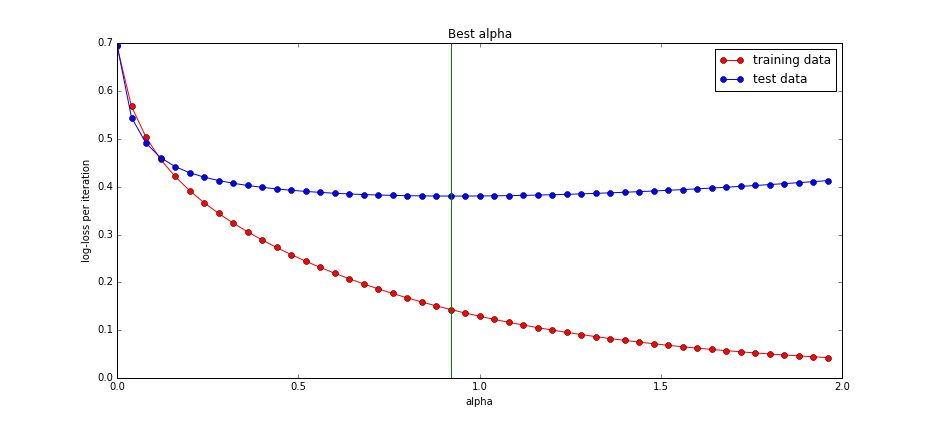
\includegraphics{./images/best_param_sgd_T.png}
\caption{Local image}
\end{figure}

    \begin{longtable}[]{@{}lcc@{}}
\toprule
& Index & \(\alpha\)\tabularnewline
\midrule
\endhead
AUC & 11 & 0.11000779999999999\tabularnewline
\bottomrule
\end{longtable}

    \begin{quote}
테스트 데이터에 최소 log-loss를 갖는 \(\alpha\)값은 0.11000779999999999
\end{quote}

    \textbf{Assumed Density Filtering}

    \begin{figure}[htbp]
\centering
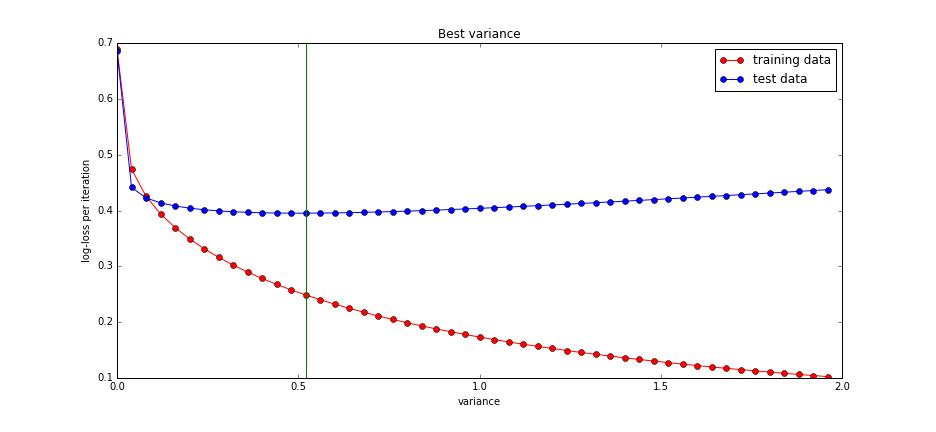
\includegraphics{./images/best_param_adf_T.png}
\caption{Local image}
\end{figure}

    \begin{longtable}[]{@{}lcc@{}}
\toprule
& Index & \(\alpha\)\tabularnewline
\midrule
\endhead
AUC & 13 & 0.52007399999999993\tabularnewline
\bottomrule
\end{longtable}

\begin{quote}
테스트 데이터에 최소 log-loss를 갖는 분산값은 0.52007399999999993
\end{quote}

    훈련 데이터 크기에 따른 log-loss 비교

    \begin{quote}
16건의 훈련 데이터를 더 사용할 때마다 그때의 회귀 계수 벡터를 이용하여
91건의 테스트 데이터에 대한 log-loss 추이를 두 방법론(SGD, ADF)에 대해
비교한다.
\end{quote}

    \begin{figure}[htbp]
\centering
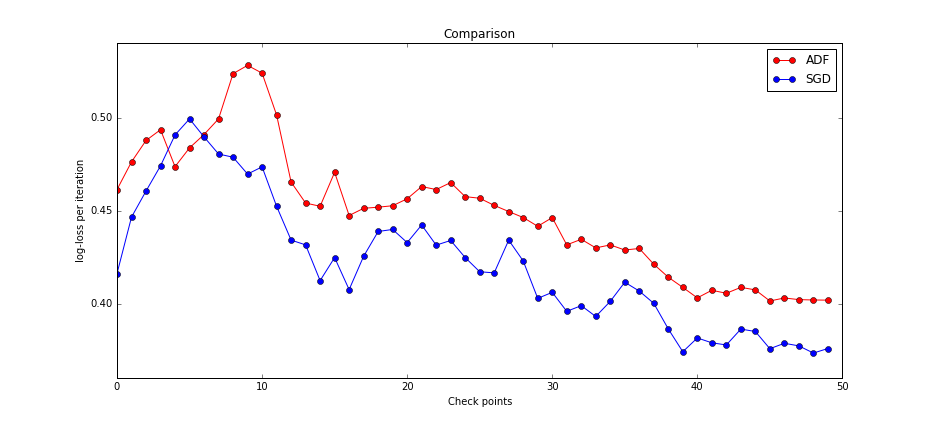
\includegraphics{./images/step_vali_comparison_T.png}
\caption{Local image}
\end{figure}

    \begin{quote}
전반적으로 ADF에 비해 SGD의 log-loss가 낮음.
\end{quote}

    \begin{figure}[htbp]
\centering
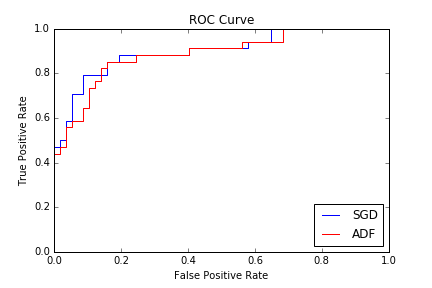
\includegraphics{./images/step_vali_roc_T.png}
\caption{Local image}
\end{figure}

    \begin{longtable}[]{@{}lcc@{}}
\toprule
& SGD & ADF\tabularnewline
\midrule
\endhead
AUC & 0.90041279669762642 & 0.88802889576883381\tabularnewline
\bottomrule
\end{longtable}

    \subsubsection{4.2. 실험(온라인 광고
데이터)}\label{uxc2e4uxd5d8uxc628uxb77cuxc778-uxad11uxace0-uxb370uxc774uxd130}

    개요

    \begin{quote}
Criteo에서 'Kaggle 대회'를 위해 공개한 4천 5백만건 상당의 온라인 광고
데이터를 사용하였다. 데이터는 웹사이트 방문자가 해당 광고를 클릭 했으냐
혹은 하지 않았느냐를 나타내는 이항 반응변수 Label과 39개의 설명변수로
구성되어 있다. 그리고 각 설명변수는 범주형으로서 범주는 500개 이상으로
실제 데이터의 경우 훈련 데이터에 없던 범주가 새롭게 등장 할 수도 있는
특성을 갖는다. 이러한 데이터를 일괄처리(batch) 방식으로 처리한다면 대략
\(19,500 \times 45,000,000\) 크기의 매트릭스 연산을 수행해야 한다.
\end{quote}

    최적 초기값

    \textbf{Stochastic Gadient Descent}

    \begin{figure}[htbp]
\centering
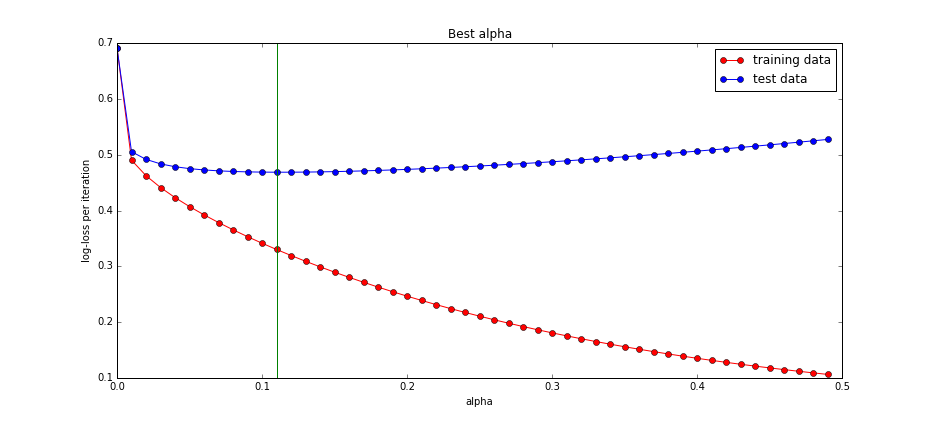
\includegraphics{./images/best_param_sgd_C.png}
\caption{Local image}
\end{figure}



    \textbf{Assumed Density Filtering}

    \begin{figure}[htbp]
\centering
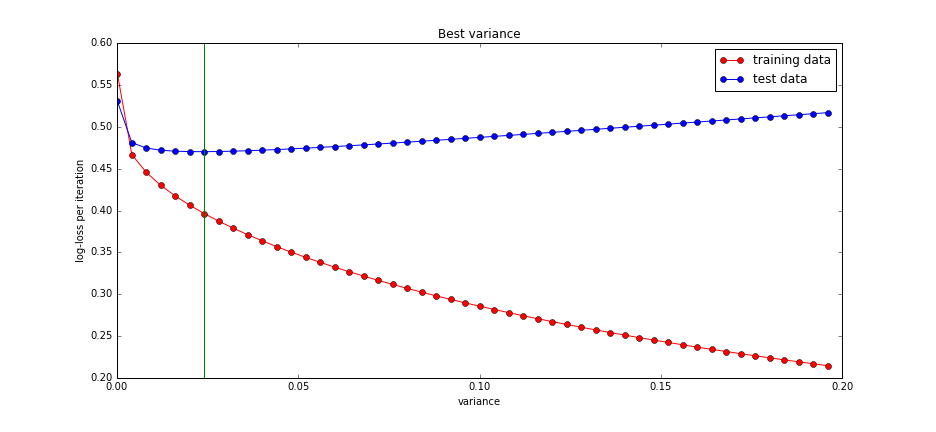
\includegraphics{./images/best_param_adf_C.png}
\caption{Local image}
\end{figure}



    훈련 데이터 크기에 따른 log-loss 비교

    \begin{figure}[htbp]
\centering
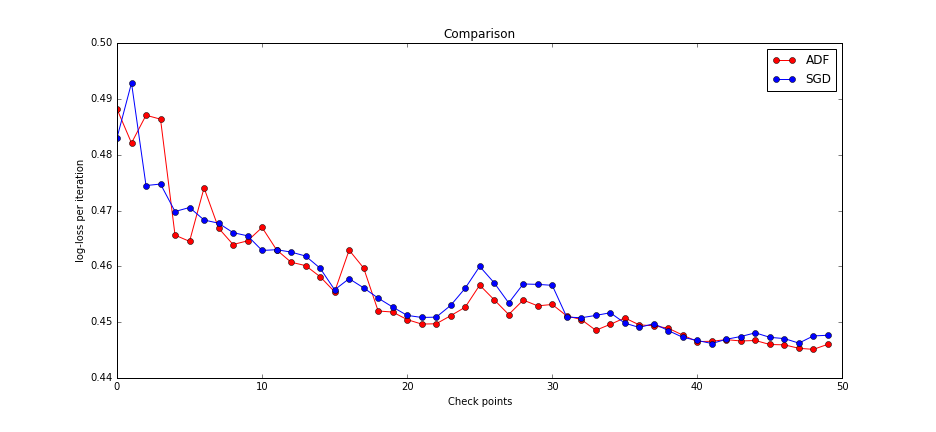
\includegraphics{./images/step_vali_comparison_C.png}
\caption{Local image}
\end{figure}

    \begin{figure}[htbp]
\centering
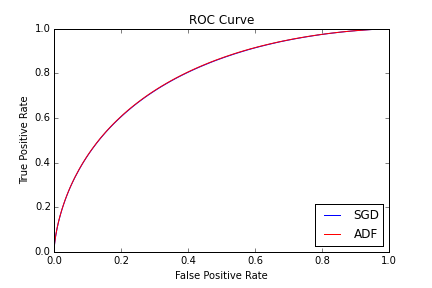
\includegraphics{./images/step_vali_roc_C.png}
\caption{Local image}
\end{figure}

    \begin{longtable}[]{@{}lcc@{}}
\toprule
& SGD & ADF\tabularnewline
\midrule
\endhead
AUC & 0.75874125874125875 & 0.75699300699300698\tabularnewline
\bottomrule
\end{longtable}

    \subsection{5. 맺음말}\label{uxb9fauxc74cuxb9d0}

    \begin{Verbatim}[commandchars=\\\{\}]
{\color{incolor}In [{\color{incolor} }]:}
\end{Verbatim}

    \begin{Verbatim}[commandchars=\\\{\}]
{\color{incolor}In [{\color{incolor} }]:}
\end{Verbatim}

    \section{{[}부록 - 구현{]}}\label{uxbd80uxb85d---uxad6cuxd604}

    \subsubsection{Simulation SGD for titanic
data}\label{simulation-sgd-for-titanic-data}

    \begin{Verbatim}[commandchars=\\\{\}]
{\color{incolor}In [{\color{incolor}8}]:} \PY{k+kn}{from} \PY{n+nn}{datetime} \PY{k+kn}{import} \PY{n}{datetime}
        \PY{k+kn}{from} \PY{n+nn}{csv} \PY{k+kn}{import} \PY{n}{DictReader}
        \PY{k+kn}{from} \PY{n+nn}{math} \PY{k+kn}{import} \PY{n}{exp}\PY{p}{,} \PY{n}{log}\PY{p}{,} \PY{n}{sqrt}
        \PY{k+kn}{import} \PY{n+nn}{numpy} \PY{k+kn}{as} \PY{n+nn}{np}
        \PY{k+kn}{import} \PY{n+nn}{mmh3}
        \PY{k+kn}{import} \PY{n+nn}{time}
        \PY{k+kn}{from} \PY{n+nn}{spooky} \PY{k+kn}{import} \PY{n}{hash128}\PY{p}{,} \PY{n}{hash64}\PY{p}{,} \PY{n}{hash32}

        \PY{k+kn}{from} \PY{n+nn}{sklearn.metrics} \PY{k+kn}{import} \PY{n}{roc\PYZus{}curve}\PY{p}{,} \PY{n}{auc}
        \PY{k+kn}{import} \PY{n+nn}{scipy.stats} \PY{k+kn}{as} \PY{n+nn}{stats}
        \PY{k+kn}{import} \PY{n+nn}{matplotlib.pyplot} \PY{k+kn}{as} \PY{n+nn}{plt}
        \PY{k+kn}{import} \PY{n+nn}{matplotlib} \PY{k+kn}{as} \PY{n+nn}{mpl}

        \PY{o}{\PYZpc{}}\PY{k}{matplotlib} inline
\end{Verbatim}

    Parameters

    \begin{Verbatim}[commandchars=\\\{\}]
{\color{incolor}In [{\color{incolor}9}]:} \PY{n}{D} \PY{o}{=} \PY{l+m+mi}{2} \PY{o}{*}\PY{o}{*} \PY{l+m+mi}{20}
        \PY{n}{rand\PYZus{}seed} \PY{o}{=} \PY{l+m+mi}{1004}

        \PY{n}{num\PYZus{}poly} \PY{o}{=} \PY{l+m+mi}{10}
        \PY{n}{xxi}\PY{p}{,} \PY{n}{wwi} \PY{o}{=} \PY{n}{np}\PY{o}{.}\PY{n}{polynomial}\PY{o}{.}\PY{n}{hermite}\PY{o}{.}\PY{n}{hermgauss}\PY{p}{(}\PY{n}{num\PYZus{}poly}\PY{p}{)}
\end{Verbatim}

    \begin{Verbatim}[commandchars=\\\{\}]
{\color{incolor}In [{\color{incolor}10}]:} \PY{k}{class} \PY{n+nc}{DataSize}\PY{p}{:}
             \PY{k}{def} \PY{n+nf}{\PYZus{}\PYZus{}init\PYZus{}\PYZus{}}\PY{p}{(}\PY{n+nb+bp}{self}
                          \PY{p}{,} \PY{n}{num\PYZus{}metric\PYZus{}check\PYZus{}point}
                          \PY{p}{,} \PY{n}{num\PYZus{}status\PYZus{}check\PYZus{}point}
                          \PY{p}{,} \PY{n}{num\PYZus{}train\PYZus{}data\PYZus{}start}
                          \PY{p}{,} \PY{n}{num\PYZus{}train\PYZus{}data\PYZus{}size}
                          \PY{p}{,} \PY{n}{num\PYZus{}test\PYZus{}data\PYZus{}start}
                          \PY{p}{,} \PY{n}{num\PYZus{}test\PYZus{}data\PYZus{}size}\PY{p}{)}\PY{p}{:}

                 \PY{n+nb+bp}{self}\PY{o}{.}\PY{n}{num\PYZus{}metric\PYZus{}check\PYZus{}point} \PY{o}{=} \PY{n}{num\PYZus{}metric\PYZus{}check\PYZus{}point}
                 \PY{n+nb+bp}{self}\PY{o}{.}\PY{n}{num\PYZus{}status\PYZus{}check\PYZus{}point} \PY{o}{=} \PY{n}{num\PYZus{}status\PYZus{}check\PYZus{}point}

                 \PY{n+nb+bp}{self}\PY{o}{.}\PY{n}{num\PYZus{}train\PYZus{}data\PYZus{}start} \PY{o}{=} \PY{n}{num\PYZus{}train\PYZus{}data\PYZus{}start}
                 \PY{n+nb+bp}{self}\PY{o}{.}\PY{n}{num\PYZus{}train\PYZus{}data\PYZus{}end} \PY{o}{=} \PY{n+nb+bp}{self}\PY{o}{.}\PY{n}{num\PYZus{}train\PYZus{}data\PYZus{}start} \PY{o}{+} \PY{n}{num\PYZus{}train\PYZus{}data\PYZus{}size} \PY{o}{\PYZhy{}} \PY{l+m+mi}{1} \PY{c+c1}{\PYZsh{} fixed}

                 \PY{n+nb+bp}{self}\PY{o}{.}\PY{n}{num\PYZus{}test\PYZus{}data\PYZus{}start} \PY{o}{=} \PY{n}{num\PYZus{}test\PYZus{}data\PYZus{}start}
                 \PY{n+nb+bp}{self}\PY{o}{.}\PY{n}{num\PYZus{}test\PYZus{}data\PYZus{}end} \PY{o}{=} \PY{n+nb+bp}{self}\PY{o}{.}\PY{n}{num\PYZus{}test\PYZus{}data\PYZus{}start} \PY{o}{+} \PY{n}{num\PYZus{}test\PYZus{}data\PYZus{}size} \PY{o}{\PYZhy{}} \PY{l+m+mi}{1} \PY{c+c1}{\PYZsh{} fixed}

             \PY{k}{def} \PY{n+nf}{display}\PY{p}{(}\PY{n+nb+bp}{self}\PY{p}{)}\PY{p}{:}
                 \PY{k}{print}\PY{p}{(}\PY{l+s+s2}{\PYZdq{}}\PY{l+s+s2}{num\PYZus{}metric\PYZus{}check\PYZus{}point: }\PY{l+s+si}{\PYZpc{}s}\PY{l+s+s2}{\PYZdq{}} \PY{o}{\PYZpc{}}\PY{p}{(}\PY{n+nb+bp}{self}\PY{o}{.}\PY{n}{num\PYZus{}metric\PYZus{}check\PYZus{}point}\PY{p}{)}\PY{p}{)}
                 \PY{k}{print}\PY{p}{(}\PY{l+s+s2}{\PYZdq{}}\PY{l+s+s2}{num\PYZus{}status\PYZus{}check\PYZus{}point: }\PY{l+s+si}{\PYZpc{}s}\PY{l+s+s2}{\PYZdq{}} \PY{o}{\PYZpc{}}\PY{p}{(}\PY{n+nb+bp}{self}\PY{o}{.}\PY{n}{num\PYZus{}status\PYZus{}check\PYZus{}point}\PY{p}{)}\PY{p}{)}
                 \PY{k}{print}\PY{p}{(}\PY{l+s+s2}{\PYZdq{}}\PY{l+s+s2}{num\PYZus{}train\PYZus{}data\PYZus{}start  : }\PY{l+s+si}{\PYZpc{}s}\PY{l+s+s2}{\PYZdq{}} \PY{o}{\PYZpc{}}\PY{p}{(}\PY{n+nb+bp}{self}\PY{o}{.}\PY{n}{num\PYZus{}train\PYZus{}data\PYZus{}start}\PY{p}{)}\PY{p}{)}
                 \PY{k}{print}\PY{p}{(}\PY{l+s+s2}{\PYZdq{}}\PY{l+s+s2}{num\PYZus{}train\PYZus{}data\PYZus{}end    : }\PY{l+s+si}{\PYZpc{}s}\PY{l+s+s2}{\PYZdq{}} \PY{o}{\PYZpc{}}\PY{p}{(}\PY{n+nb+bp}{self}\PY{o}{.}\PY{n}{num\PYZus{}train\PYZus{}data\PYZus{}end}\PY{p}{)}\PY{p}{)}
                 \PY{k}{print}\PY{p}{(}\PY{l+s+s2}{\PYZdq{}}\PY{l+s+s2}{num\PYZus{}train\PYZus{}data\PYZus{}size   : }\PY{l+s+si}{\PYZpc{}s}\PY{l+s+s2}{\PYZdq{}} \PY{o}{\PYZpc{}}\PY{p}{(}\PY{n+nb+bp}{self}\PY{o}{.}\PY{n}{num\PYZus{}train\PYZus{}data\PYZus{}end} \PY{o}{\PYZhy{}} \PY{n+nb+bp}{self}\PY{o}{.}\PY{n}{num\PYZus{}train\PYZus{}data\PYZus{}start} \PY{o}{+} \PY{l+m+mi}{1}\PY{p}{)}\PY{p}{)}
                 \PY{k}{print}\PY{p}{(}\PY{l+s+s2}{\PYZdq{}}\PY{l+s+s2}{num\PYZus{}test\PYZus{}data\PYZus{}start   : }\PY{l+s+si}{\PYZpc{}s}\PY{l+s+s2}{\PYZdq{}} \PY{o}{\PYZpc{}}\PY{p}{(}\PY{n+nb+bp}{self}\PY{o}{.}\PY{n}{num\PYZus{}test\PYZus{}data\PYZus{}start}\PY{p}{)}\PY{p}{)}
                 \PY{k}{print}\PY{p}{(}\PY{l+s+s2}{\PYZdq{}}\PY{l+s+s2}{num\PYZus{}test\PYZus{}data\PYZus{}end     : }\PY{l+s+si}{\PYZpc{}s}\PY{l+s+s2}{\PYZdq{}} \PY{o}{\PYZpc{}}\PY{p}{(}\PY{n+nb+bp}{self}\PY{o}{.}\PY{n}{num\PYZus{}test\PYZus{}data\PYZus{}end}\PY{p}{)}\PY{p}{)}
                 \PY{k}{print}\PY{p}{(}\PY{l+s+s2}{\PYZdq{}}\PY{l+s+s2}{num\PYZus{}test\PYZus{}data\PYZus{}size    : }\PY{l+s+si}{\PYZpc{}s}\PY{l+s+s2}{\PYZdq{}} \PY{o}{\PYZpc{}}\PY{p}{(}\PY{n+nb+bp}{self}\PY{o}{.}\PY{n}{num\PYZus{}test\PYZus{}data\PYZus{}end} \PY{o}{\PYZhy{}} \PY{n+nb+bp}{self}\PY{o}{.}\PY{n}{num\PYZus{}test\PYZus{}data\PYZus{}start} \PY{o}{+} \PY{l+m+mi}{1}\PY{p}{)}\PY{p}{)}
\end{Verbatim}

    \begin{Verbatim}[commandchars=\\\{\}]
{\color{incolor}In [{\color{incolor}11}]:} \PY{k}{class} \PY{n+nc}{FileInfo}\PY{p}{:}
             \PY{k}{def} \PY{n+nf}{\PYZus{}\PYZus{}init\PYZus{}\PYZus{}}\PY{p}{(}\PY{n+nb+bp}{self}
                         \PY{p}{,} \PY{n}{\PYZus{}file\PYZus{}path}
                         \PY{p}{,} \PY{n}{\PYZus{}f\PYZus{}having\PYZus{}header}
                         \PY{p}{,} \PY{n}{\PYZus{}l\PYZus{}header\PYZus{}names}
                         \PY{p}{,} \PY{n}{\PYZus{}seperator}
                         \PY{p}{,} \PY{n}{\PYZus{}l\PYZus{}skip\PYZus{}columns}
                         \PY{p}{,} \PY{n}{\PYZus{}ylab}\PY{p}{)}\PY{p}{:}
                 \PY{n+nb+bp}{self}\PY{o}{.}\PY{n}{file\PYZus{}path} \PY{o}{=} \PY{n}{\PYZus{}file\PYZus{}path}
                 \PY{n+nb+bp}{self}\PY{o}{.}\PY{n}{f\PYZus{}having\PYZus{}header} \PY{o}{=} \PY{n}{\PYZus{}f\PYZus{}having\PYZus{}header}
                 \PY{n+nb+bp}{self}\PY{o}{.}\PY{n}{l\PYZus{}header\PYZus{}names} \PY{o}{=} \PY{n}{\PYZus{}l\PYZus{}header\PYZus{}names}
                 \PY{n+nb+bp}{self}\PY{o}{.}\PY{n}{seperator} \PY{o}{=} \PY{n}{\PYZus{}seperator}
                 \PY{n+nb+bp}{self}\PY{o}{.}\PY{n}{l\PYZus{}skip\PYZus{}columns} \PY{o}{=} \PY{n}{\PYZus{}l\PYZus{}skip\PYZus{}columns}
                 \PY{n+nb+bp}{self}\PY{o}{.}\PY{n}{ylab} \PY{o}{=} \PY{n}{\PYZus{}ylab}

\end{Verbatim}

    \begin{Verbatim}[commandchars=\\\{\}]
{\color{incolor}In [{\color{incolor}12}]:} \PY{n}{fi\PYZus{}titanic} \PY{o}{=} \PY{n}{FileInfo}\PY{p}{(}
                         \PY{l+s+s1}{r\PYZsq{}}\PY{l+s+s1}{C:/My/Playground/Git/2016\PYZus{}Thesis/100\PYZus{}Simulation/data/train.csv}\PY{l+s+s1}{\PYZsq{}} \PY{c+c1}{\PYZsh{} \PYZus{}file\PYZus{}path}
                         \PY{p}{,} \PY{n+nb+bp}{True} \PY{c+c1}{\PYZsh{} \PYZus{}f\PYZus{}having\PYZus{}header}
                         \PY{p}{,} \PY{p}{[}\PY{l+s+s1}{\PYZsq{}}\PY{l+s+s1}{PassengerId}\PY{l+s+s1}{\PYZsq{}}\PY{p}{,} \PY{l+s+s1}{\PYZsq{}}\PY{l+s+s1}{Survived}\PY{l+s+s1}{\PYZsq{}}\PY{p}{,} \PY{l+s+s1}{\PYZsq{}}\PY{l+s+s1}{Pclass}\PY{l+s+s1}{\PYZsq{}}\PY{p}{,} \PY{l+s+s1}{\PYZsq{}}\PY{l+s+s1}{Name}\PY{l+s+s1}{\PYZsq{}}\PY{p}{,} \PY{l+s+s1}{\PYZsq{}}\PY{l+s+s1}{Sex}\PY{l+s+s1}{\PYZsq{}}
                            \PY{p}{,} \PY{l+s+s1}{\PYZsq{}}\PY{l+s+s1}{Age}\PY{l+s+s1}{\PYZsq{}}\PY{p}{,} \PY{l+s+s1}{\PYZsq{}}\PY{l+s+s1}{SibSp}\PY{l+s+s1}{\PYZsq{}}\PY{p}{,} \PY{l+s+s1}{\PYZsq{}}\PY{l+s+s1}{Parch}\PY{l+s+s1}{\PYZsq{}}\PY{p}{,} \PY{l+s+s1}{\PYZsq{}}\PY{l+s+s1}{Ticket}\PY{l+s+s1}{\PYZsq{}}\PY{p}{,} \PY{l+s+s1}{\PYZsq{}}\PY{l+s+s1}{Fare}\PY{l+s+s1}{\PYZsq{}}\PY{p}{,} \PY{l+s+s1}{\PYZsq{}}\PY{l+s+s1}{Cabin}\PY{l+s+s1}{\PYZsq{}} \PY{p}{,} \PY{l+s+s1}{\PYZsq{}}\PY{l+s+s1}{Embarked}\PY{l+s+s1}{\PYZsq{}}\PY{p}{]} \PY{c+c1}{\PYZsh{} \PYZus{}l\PYZus{}header\PYZus{}names}
                         \PY{p}{,} \PY{l+s+s1}{\PYZsq{}}\PY{l+s+s1}{,}\PY{l+s+s1}{\PYZsq{}} \PY{c+c1}{\PYZsh{} \PYZus{}seperator}
                         \PY{p}{,} \PY{p}{[}\PY{l+s+s1}{\PYZsq{}}\PY{l+s+s1}{PassengerId}\PY{l+s+s1}{\PYZsq{}}\PY{p}{]}\PY{c+c1}{\PYZsh{} \PYZus{}l\PYZus{}skip\PYZus{}columns}
                         \PY{p}{,} \PY{l+s+s1}{\PYZsq{}}\PY{l+s+s1}{Survived}\PY{l+s+s1}{\PYZsq{}}\PY{c+c1}{\PYZsh{} \PYZus{}ylab}
                         \PY{p}{)}

         \PY{n}{fi\PYZus{}criteo} \PY{o}{=} \PY{n}{FileInfo}\PY{p}{(}
                         \PY{l+s+s1}{r\PYZsq{}}\PY{l+s+s1}{C:}\PY{l+s+s1}{\PYZbs{}}\PY{l+s+s1}{Temp}\PY{l+s+s1}{\PYZbs{}}\PY{l+s+s1}{dac.tar}\PY{l+s+s1}{\PYZbs{}}\PY{l+s+s1}{train.txt}\PY{l+s+s1}{\PYZsq{}} \PY{c+c1}{\PYZsh{} \PYZus{}file\PYZus{}path}
                         \PY{p}{,} \PY{n+nb+bp}{False} \PY{c+c1}{\PYZsh{} \PYZus{}f\PYZus{}having\PYZus{}header}
                         \PY{p}{,} \PY{p}{[}\PY{l+s+s1}{\PYZsq{}}\PY{l+s+s1}{Label}\PY{l+s+s1}{\PYZsq{}}\PY{p}{]} \PY{o}{+} \PY{p}{[} \PY{l+s+s1}{\PYZsq{}}\PY{l+s+s1}{I}\PY{l+s+s1}{\PYZsq{}} \PY{o}{+} \PY{n+nb}{str}\PY{p}{(}\PY{n}{i}\PY{p}{)} \PY{k}{for} \PY{n}{i} \PY{o+ow}{in} \PY{n+nb}{list}\PY{p}{(}\PY{n+nb}{range}\PY{p}{(}\PY{l+m+mi}{1}\PY{p}{,}\PY{l+m+mi}{14}\PY{p}{)}\PY{p}{)}\PY{p}{]} \PY{o}{+} \PY{p}{[} \PY{l+s+s1}{\PYZsq{}}\PY{l+s+s1}{C}\PY{l+s+s1}{\PYZsq{}} \PY{o}{+} \PY{n+nb}{str}\PY{p}{(}\PY{n}{i}\PY{p}{)} \PY{k}{for} \PY{n}{i} \PY{o+ow}{in} \PY{n+nb}{list}\PY{p}{(}\PY{n+nb}{range}\PY{p}{(}\PY{l+m+mi}{1}\PY{p}{,}\PY{l+m+mi}{27}\PY{p}{)}\PY{p}{)}\PY{p}{]} \PY{c+c1}{\PYZsh{} \PYZus{}l\PYZus{}header\PYZus{}names}
                         \PY{p}{,} \PY{l+s+s1}{\PYZsq{}}\PY{l+s+se}{\PYZbs{}t}\PY{l+s+s1}{\PYZsq{}} \PY{c+c1}{\PYZsh{} \PYZus{}seperator}
                         \PY{p}{,} \PY{p}{[}\PY{p}{]}\PY{c+c1}{\PYZsh{} \PYZus{}l\PYZus{}skip\PYZus{}columns}
                         \PY{p}{,} \PY{l+s+s1}{\PYZsq{}}\PY{l+s+s1}{Label}\PY{l+s+s1}{\PYZsq{}}\PY{c+c1}{\PYZsh{} \PYZus{}ylab}
                         \PY{p}{)}
\end{Verbatim}

    Functions

    \begin{Verbatim}[commandchars=\\\{\}]
{\color{incolor}In [{\color{incolor}13}]:} \PY{c+c1}{\PYZsh{} csv\PYZus{}row must be dict}
         \PY{k}{def} \PY{n+nf}{get\PYZus{}x\PYZus{}mmh3}\PY{p}{(}\PY{n}{csv\PYZus{}row}\PY{p}{,} \PY{n}{D}\PY{p}{)}\PY{p}{:}
             \PY{n}{x} \PY{o}{=} \PY{p}{[}\PY{l+m+mi}{0}\PY{p}{]}
             \PY{k}{for} \PY{n}{key}\PY{p}{,} \PY{n}{value} \PY{o+ow}{in} \PY{n}{csv\PYZus{}row}\PY{o}{.}\PY{n}{items}\PY{p}{(}\PY{p}{)}\PY{p}{:}
                 \PY{n}{index} \PY{o}{=} \PY{n}{mmh3}\PY{o}{.}\PY{n}{hash128}\PY{p}{(}\PY{n+nb}{str}\PY{p}{(}\PY{n}{key}\PY{p}{)} \PY{o}{+} \PY{n+nb}{str}\PY{p}{(}\PY{n}{value}\PY{p}{)}\PY{p}{,} \PY{n}{seed}\PY{o}{=}\PY{n}{rand\PYZus{}seed}\PY{p}{,} \PY{n}{x64arch}\PY{o}{=}\PY{n+nb+bp}{True}\PY{p}{)} \PY{o}{\PYZpc{}} \PY{n}{D}
                 \PY{n}{x}\PY{o}{.}\PY{n}{append}\PY{p}{(}\PY{n}{index}\PY{p}{)}
             \PY{k}{return} \PY{n}{x}
\end{Verbatim}

    \begin{Verbatim}[commandchars=\\\{\}]
{\color{incolor}In [{\color{incolor}14}]:} \PY{c+c1}{\PYZsh{} csv\PYZus{}row must be dict}
         \PY{k}{def} \PY{n+nf}{get\PYZus{}x\PYZus{}spooky}\PY{p}{(}\PY{n}{csv\PYZus{}row}\PY{p}{,} \PY{n}{D}\PY{p}{)}\PY{p}{:}
             \PY{n}{x} \PY{o}{=} \PY{p}{[}\PY{l+m+mi}{0}\PY{p}{]}
             \PY{k}{for} \PY{n}{key}\PY{p}{,} \PY{n}{value} \PY{o+ow}{in} \PY{n}{csv\PYZus{}row}\PY{o}{.}\PY{n}{items}\PY{p}{(}\PY{p}{)}\PY{p}{:}
                 \PY{n}{index} \PY{o}{=} \PY{n}{hash32}\PY{p}{(}\PY{n+nb}{str}\PY{p}{(}\PY{n}{key}\PY{p}{)} \PY{o}{+} \PY{n+nb}{str}\PY{p}{(}\PY{n}{value}\PY{p}{)}\PY{p}{)} \PY{o}{\PYZpc{}} \PY{n}{D}
                 \PY{n}{x}\PY{o}{.}\PY{n}{append}\PY{p}{(}\PY{n}{index}\PY{p}{)}
             \PY{k}{return} \PY{n}{x}
\end{Verbatim}

    \begin{Verbatim}[commandchars=\\\{\}]
{\color{incolor}In [{\color{incolor}15}]:} \PY{k}{def} \PY{n+nf}{get\PYZus{}p}\PY{p}{(}\PY{n}{x}\PY{p}{,} \PY{n}{w}\PY{p}{)}\PY{p}{:}
             \PY{n}{wTx} \PY{o}{=} \PY{l+m+mf}{0.}
             \PY{k}{for} \PY{n}{i} \PY{o+ow}{in} \PY{n}{x}\PY{p}{:}  \PY{c+c1}{\PYZsh{} do wTx}
                 \PY{n}{wTx} \PY{o}{+}\PY{o}{=} \PY{n}{w}\PY{p}{[}\PY{n}{i}\PY{p}{]} \PY{o}{*} \PY{l+m+mf}{1.}  \PY{c+c1}{\PYZsh{} w[i] * x[i], but if i in x we got x[i] = 1.}
             \PY{k}{return} \PY{l+m+mf}{1.} \PY{o}{/} \PY{p}{(}\PY{l+m+mf}{1.} \PY{o}{+} \PY{n}{exp}\PY{p}{(}\PY{o}{\PYZhy{}}\PY{n+nb}{max}\PY{p}{(}\PY{n+nb}{min}\PY{p}{(}\PY{n}{wTx}\PY{p}{,} \PY{l+m+mf}{20.}\PY{p}{)}\PY{p}{,} \PY{o}{\PYZhy{}}\PY{l+m+mf}{20.}\PY{p}{)}\PY{p}{)}\PY{p}{)}  \PY{c+c1}{\PYZsh{} bounded sigmoid}
\end{Verbatim}

    \begin{Verbatim}[commandchars=\\\{\}]
{\color{incolor}In [{\color{incolor}16}]:} \PY{c+c1}{\PYZsh{} w must be numpy ndarray}
         \PY{k}{def} \PY{n+nf}{get\PYZus{}p\PYZus{}cat}\PY{p}{(}\PY{n}{x}\PY{p}{,} \PY{n}{w}\PY{p}{)}\PY{p}{:}
             \PY{n}{wTx} \PY{o}{=} \PY{n+nb}{sum}\PY{p}{(}\PY{n}{w}\PY{p}{[}\PY{n}{x}\PY{p}{]}\PY{p}{)}
             \PY{k}{return} \PY{l+m+mf}{1.} \PY{o}{/} \PY{p}{(}\PY{l+m+mf}{1.} \PY{o}{+} \PY{n}{exp}\PY{p}{(}\PY{o}{\PYZhy{}}\PY{n+nb}{max}\PY{p}{(}\PY{n+nb}{min}\PY{p}{(}\PY{n}{wTx}\PY{p}{,} \PY{l+m+mf}{20.}\PY{p}{)}\PY{p}{,} \PY{o}{\PYZhy{}}\PY{l+m+mf}{20.}\PY{p}{)}\PY{p}{)}\PY{p}{)}  \PY{c+c1}{\PYZsh{} bounded sigmoid}
\end{Verbatim}

    \begin{Verbatim}[commandchars=\\\{\}]
{\color{incolor}In [{\color{incolor}17}]:} \PY{k}{def} \PY{n+nf}{logloss}\PY{p}{(}\PY{n}{p}\PY{p}{,} \PY{n}{y}\PY{p}{)}\PY{p}{:}
             \PY{n}{p} \PY{o}{=} \PY{n+nb}{max}\PY{p}{(}\PY{n+nb}{min}\PY{p}{(}\PY{n}{p}\PY{p}{,} \PY{l+m+mf}{1.} \PY{o}{\PYZhy{}} \PY{l+m+mf}{10e\PYZhy{}12}\PY{p}{)}\PY{p}{,} \PY{l+m+mf}{10e\PYZhy{}12}\PY{p}{)}
             \PY{k}{return} \PY{o}{\PYZhy{}}\PY{n}{log}\PY{p}{(}\PY{n}{p}\PY{p}{)} \PY{k}{if} \PY{n}{y} \PY{o}{==} \PY{l+m+mf}{1.} \PY{k}{else} \PY{o}{\PYZhy{}}\PY{n}{log}\PY{p}{(}\PY{l+m+mf}{1.} \PY{o}{\PYZhy{}} \PY{n}{p}\PY{p}{)}
\end{Verbatim}

    \begin{Verbatim}[commandchars=\\\{\}]
{\color{incolor}In [{\color{incolor}18}]:} \PY{k}{def} \PY{n+nf}{get\PYZus{}validation\PYZus{}metrics}\PY{p}{(}\PY{n}{c\PYZus{}fi}\PY{p}{,}\PY{n}{start}\PY{p}{,} \PY{n}{end}\PY{p}{,} \PY{n}{wlen}\PY{p}{,} \PY{n}{w}\PY{p}{,} \PY{n}{f\PYZus{}debug}\PY{p}{)}\PY{p}{:}

             \PY{n}{log\PYZus{}loss} \PY{o}{=} \PY{l+m+mf}{0.}
             \PY{n}{arr\PYZus{}y} \PY{o}{=} \PY{p}{[}\PY{p}{]}
             \PY{n}{arr\PYZus{}p} \PY{o}{=} \PY{p}{[}\PY{p}{]}

             \PY{n}{f} \PY{o}{=} \PY{n+nb}{open}\PY{p}{(}\PY{n}{c\PYZus{}fi}\PY{o}{.}\PY{n}{file\PYZus{}path}\PY{p}{)}
             \PY{k}{for} \PY{n}{t}\PY{p}{,} \PY{n}{row} \PY{o+ow}{in} \PY{n+nb}{enumerate}\PY{p}{(}\PY{n}{DictReader}\PY{p}{(}\PY{n}{f}\PY{p}{,} \PY{n}{fieldnames}\PY{o}{=}\PY{n}{c\PYZus{}fi}\PY{o}{.}\PY{n}{l\PYZus{}header\PYZus{}names}\PY{p}{,} \PY{n}{delimiter}\PY{o}{=}\PY{n}{c\PYZus{}fi}\PY{o}{.}\PY{n}{seperator}\PY{p}{)}\PY{p}{)}\PY{p}{:}
                 \PY{k}{if} \PY{n}{t} \PY{o}{==} \PY{l+m+mi}{0}\PY{p}{:}
                     \PY{k}{continue} \PY{c+c1}{\PYZsh{} just for titanic}

                 \PY{k}{if} \PY{n}{t} \PY{o}{\PYZlt{}} \PY{n}{start}\PY{p}{:} \PY{c+c1}{\PYZsh{} fixed}
                     \PY{k}{continue}\PY{p}{;}

                 \PY{n}{y} \PY{o}{=} \PY{l+m+mf}{1.} \PY{k}{if} \PY{n}{row}\PY{p}{[}\PY{n}{c\PYZus{}fi}\PY{o}{.}\PY{n}{ylab}\PY{p}{]} \PY{o}{==} \PY{l+s+s1}{\PYZsq{}}\PY{l+s+s1}{1}\PY{l+s+s1}{\PYZsq{}} \PY{k}{else} \PY{l+m+mf}{0.}
                 \PY{k}{del} \PY{n}{row}\PY{p}{[}\PY{n}{c\PYZus{}fi}\PY{o}{.}\PY{n}{ylab}\PY{p}{]}
                 \PY{n}{arr\PYZus{}y}\PY{o}{.}\PY{n}{append}\PY{p}{(}\PY{n}{y}\PY{p}{)}

                 \PY{k}{if}\PY{p}{(}\PY{n+nb}{len}\PY{p}{(}\PY{n}{c\PYZus{}fi}\PY{o}{.}\PY{n}{l\PYZus{}skip\PYZus{}columns}\PY{p}{)} \PY{o}{\PYZgt{}} \PY{l+m+mi}{0}\PY{p}{)}\PY{p}{:}
                     \PY{k}{for} \PY{n}{i} \PY{o+ow}{in} \PY{n+nb}{range}\PY{p}{(}\PY{n+nb}{len}\PY{p}{(}\PY{n}{c\PYZus{}fi}\PY{o}{.}\PY{n}{l\PYZus{}skip\PYZus{}columns}\PY{p}{)}\PY{p}{)}\PY{p}{:}
                         \PY{k}{del} \PY{n}{row}\PY{p}{[}\PY{p}{(}\PY{n}{c\PYZus{}fi}\PY{o}{.}\PY{n}{l\PYZus{}skip\PYZus{}columns}\PY{p}{)}\PY{p}{[}\PY{n}{i}\PY{p}{]}\PY{p}{]} \PY{c+c1}{\PYZsh{} for titanic}

                 \PY{n}{x} \PY{o}{=} \PY{n}{get\PYZus{}x\PYZus{}mmh3}\PY{p}{(}\PY{n}{row}\PY{p}{,} \PY{n}{wlen}\PY{p}{)}

                 \PY{n}{p} \PY{o}{=} \PY{l+m+mi}{0}
                 \PY{k}{if}\PY{p}{(}\PY{n+nb}{isinstance}\PY{p}{(}\PY{n}{w}\PY{p}{,} \PY{n+nb}{list}\PY{p}{)}\PY{p}{)}\PY{p}{:}
                     \PY{n}{p} \PY{o}{=} \PY{n}{get\PYZus{}p}\PY{p}{(}\PY{n}{x}\PY{p}{,} \PY{n}{w}\PY{p}{)}
                 \PY{k}{else}\PY{p}{:}
                     \PY{n}{p} \PY{o}{=} \PY{n}{get\PYZus{}p\PYZus{}cat}\PY{p}{(}\PY{n}{x}\PY{p}{,} \PY{n}{w}\PY{p}{)}
                 \PY{n}{arr\PYZus{}p}\PY{o}{.}\PY{n}{append}\PY{p}{(}\PY{n}{p}\PY{p}{)}

                 \PY{n}{log\PYZus{}loss} \PY{o}{+}\PY{o}{=} \PY{n}{logloss}\PY{p}{(}\PY{n}{p}\PY{p}{,} \PY{n}{y}\PY{p}{)}

                 \PY{k}{if} \PY{n}{f\PYZus{}debug}\PY{p}{:}
                     \PY{k}{if} \PY{n}{t} \PY{o}{\PYZgt{}}\PY{o}{=} \PY{l+m+mi}{1}\PY{p}{:}  \PY{c+c1}{\PYZsh{} fixed}
                         \PY{k}{print}\PY{p}{(}\PY{l+s+s1}{\PYZsq{}}\PY{l+s+s1}{ [get\PYZus{}validation\PYZus{}metrics] }\PY{l+s+si}{\PYZpc{}s}\PY{l+s+se}{\PYZbs{}t}\PY{l+s+s1}{encountered: }\PY{l+s+si}{\PYZpc{}d}\PY{l+s+se}{\PYZbs{}t}\PY{l+s+s1}{ y=}\PY{l+s+si}{\PYZpc{}d}\PY{l+s+s1}{: }\PY{l+s+si}{\PYZpc{}f}\PY{l+s+s1}{, loss:}\PY{l+s+si}{\PYZpc{}f}\PY{l+s+s1}{\PYZsq{}} \PY{o}{\PYZpc{}} \PY{p}{(}
                             \PY{n}{datetime}\PY{o}{.}\PY{n}{now}\PY{p}{(}\PY{p}{)}\PY{p}{,} \PY{p}{(}\PY{n}{t}\PY{p}{)}\PY{p}{,} \PY{n}{y}\PY{p}{,} \PY{n}{p}\PY{p}{,} \PY{n}{log\PYZus{}loss}\PY{o}{/}\PY{n}{t}\PY{p}{)}\PY{p}{)}

                 \PY{c+c1}{\PYZsh{} End of ...}
                 \PY{k}{if} \PY{n}{t} \PY{o}{\PYZgt{}}\PY{o}{=} \PY{n}{end}\PY{p}{:} \PY{c+c1}{\PYZsh{} fixed}
                     \PY{k}{break}\PY{p}{;}

             \PY{n}{f}\PY{o}{.}\PY{n}{close}\PY{p}{(}\PY{p}{)}

             \PY{k}{return}\PY{p}{(}\PY{n}{log\PYZus{}loss}\PY{p}{,} \PY{n}{arr\PYZus{}y}\PY{p}{,} \PY{n}{arr\PYZus{}p}\PY{p}{)}

         \PY{c+c1}{\PYZsh{}fn = [\PYZsq{}Label\PYZsq{}] + [ \PYZsq{}I\PYZsq{} + str(i) for i in list(range(1,14))] + [ \PYZsq{}C\PYZsq{} + str(i) for i in list(range(1,27))]}
         \PY{c+c1}{\PYZsh{}get\PYZus{}validation\PYZus{}metrics(train, fn, \PYZsq{}\PYZbs{}t\PYZsq{}, \PYZsq{}Label\PYZsq{}, num\PYZus{}test\PYZus{}data\PYZus{}start, num\PYZus{}test\PYZus{}data\PYZus{}end, D, w)}
\end{Verbatim}

    \begin{Verbatim}[commandchars=\\\{\}]
{\color{incolor}In [{\color{incolor}19}]:} \PY{k}{def} \PY{n+nf}{plot\PYZus{}log\PYZus{}loss}\PY{p}{(}\PY{n}{arr\PYZus{}log\PYZus{}loss}\PY{p}{)}\PY{p}{:}
             \PY{n}{plt}\PY{o}{.}\PY{n}{figure}\PY{p}{(}\PY{n}{num}\PY{o}{=}\PY{n+nb+bp}{None}\PY{p}{,} \PY{n}{figsize}\PY{o}{=}\PY{p}{(}\PY{l+m+mi}{13}\PY{p}{,} \PY{l+m+mi}{6}\PY{p}{)}\PY{p}{,} \PY{n}{dpi}\PY{o}{=}\PY{l+m+mi}{80}\PY{p}{,} \PY{n}{facecolor}\PY{o}{=}\PY{l+s+s1}{\PYZsq{}}\PY{l+s+s1}{w}\PY{l+s+s1}{\PYZsq{}}\PY{p}{,} \PY{n}{edgecolor}\PY{o}{=}\PY{l+s+s1}{\PYZsq{}}\PY{l+s+s1}{k}\PY{l+s+s1}{\PYZsq{}}\PY{p}{)}
             \PY{n}{x} \PY{o}{=} \PY{n+nb}{range}\PY{p}{(}\PY{n+nb}{len}\PY{p}{(}\PY{n}{arr\PYZus{}log\PYZus{}loss}\PY{p}{)}\PY{p}{)}
             \PY{n}{plt}\PY{o}{.}\PY{n}{plot}\PY{p}{(}\PY{n}{x}\PY{p}{,} \PY{n}{arr\PYZus{}log\PYZus{}loss}\PY{p}{,} \PY{n}{label}\PY{o}{=}\PY{l+s+s1}{\PYZsq{}}\PY{l+s+s1}{log\PYZus{}loss}\PY{l+s+s1}{\PYZsq{}}\PY{p}{,} \PY{n}{marker}\PY{o}{=}\PY{l+s+s1}{\PYZsq{}}\PY{l+s+s1}{o}\PY{l+s+s1}{\PYZsq{}}\PY{p}{)}
\end{Verbatim}

    \section{SGD}\label{sgd}

    Functions

    \begin{Verbatim}[commandchars=\\\{\}]
{\color{incolor}In [{\color{incolor}20}]:} \PY{k}{def} \PY{n+nf}{update\PYZus{}w\PYZus{}withn}\PY{p}{(}\PY{n}{w}\PY{p}{,} \PY{n}{n}\PY{p}{,} \PY{n}{x}\PY{p}{,} \PY{n}{p}\PY{p}{,} \PY{n}{y}\PY{p}{,} \PY{n}{alpha}\PY{p}{)}\PY{p}{:}
             \PY{k}{for} \PY{n}{i} \PY{o+ow}{in} \PY{n}{x}\PY{p}{:}
                 \PY{n}{w}\PY{p}{[}\PY{n}{i}\PY{p}{]} \PY{o}{\PYZhy{}}\PY{o}{=} \PY{p}{(}\PY{n}{p} \PY{o}{\PYZhy{}} \PY{n}{y}\PY{p}{)} \PY{o}{*} \PY{n}{alpha} \PY{o}{/} \PY{p}{(}\PY{n}{sqrt}\PY{p}{(}\PY{n}{n}\PY{p}{[}\PY{n}{i}\PY{p}{]}\PY{p}{)} \PY{o}{+} \PY{l+m+mf}{1.}\PY{p}{)}
                 \PY{n}{n}\PY{p}{[}\PY{n}{i}\PY{p}{]} \PY{o}{+}\PY{o}{=} \PY{l+m+mf}{1.}
             \PY{k}{return} \PY{n}{w}\PY{p}{,} \PY{n}{n}
\end{Verbatim}

    \begin{Verbatim}[commandchars=\\\{\}]
{\color{incolor}In [{\color{incolor}21}]:} \PY{k}{def} \PY{n+nf}{update\PYZus{}w}\PY{p}{(}\PY{n}{w}\PY{p}{,} \PY{n}{n}\PY{p}{,} \PY{n}{x}\PY{p}{,} \PY{n}{p}\PY{p}{,} \PY{n}{y}\PY{p}{,} \PY{n}{alpha}\PY{p}{)}\PY{p}{:}
             \PY{k}{for} \PY{n}{i} \PY{o+ow}{in} \PY{n}{x}\PY{p}{:}
                 \PY{n}{w}\PY{p}{[}\PY{n}{i}\PY{p}{]} \PY{o}{\PYZhy{}}\PY{o}{=} \PY{p}{(}\PY{n}{p} \PY{o}{\PYZhy{}} \PY{n}{y}\PY{p}{)} \PY{o}{*} \PY{n}{alpha}
                 \PY{n}{n}\PY{p}{[}\PY{n}{i}\PY{p}{]} \PY{o}{+}\PY{o}{=} \PY{l+m+mf}{1.}
             \PY{k}{return} \PY{n}{w}\PY{p}{,} \PY{n}{n}
\end{Verbatim}

    Training function

    \begin{Verbatim}[commandchars=\\\{\}]
{\color{incolor}In [{\color{incolor}22}]:} \PY{k}{def} \PY{n+nf}{sgd\PYZus{}training}\PY{p}{(}\PY{n}{alpha}\PY{p}{,} \PY{n}{D}\PY{p}{,} \PY{n}{f\PYZus{}debug}\PY{p}{,} \PY{n}{f\PYZus{}step\PYZus{}validation}\PY{p}{,} \PY{n}{f\PYZus{}validation}\PY{p}{,} \PY{n}{c\PYZus{}ds}\PY{p}{,} \PY{n}{c\PYZus{}fi}\PY{p}{)}\PY{p}{:}
             \PY{n}{w} \PY{o}{=} \PY{p}{[}\PY{l+m+mf}{0.}\PY{p}{]} \PY{o}{*} \PY{n}{D}  \PY{c+c1}{\PYZsh{} weights}
             \PY{n}{n} \PY{o}{=} \PY{n}{np}\PY{o}{.}\PY{n}{array}\PY{p}{(}\PY{p}{[}\PY{l+m+mf}{0.}\PY{p}{]} \PY{o}{*} \PY{p}{(}\PY{n}{D}\PY{p}{)}\PY{p}{)}

             \PY{n}{start\PYZus{}time} \PY{o}{=} \PY{n}{time}\PY{o}{.}\PY{n}{time}\PY{p}{(}\PY{p}{)}

             \PY{n}{log\PYZus{}loss\PYZus{}sgd\PYZus{}training} \PY{o}{=} \PY{l+m+mf}{0.}
             \PY{n}{arr\PYZus{}log\PYZus{}loss\PYZus{}sgd\PYZus{}test} \PY{o}{=} \PY{p}{[}\PY{p}{]}

             \PY{n}{f} \PY{o}{=} \PY{n+nb}{open}\PY{p}{(}\PY{n}{c\PYZus{}fi}\PY{o}{.}\PY{n}{file\PYZus{}path}\PY{p}{)}
             \PY{n}{fn} \PY{o}{=} \PY{n}{c\PYZus{}fi}\PY{o}{.}\PY{n}{l\PYZus{}header\PYZus{}names}

             \PY{k}{for} \PY{n}{t}\PY{p}{,} \PY{n}{row} \PY{o+ow}{in} \PY{n+nb}{enumerate}\PY{p}{(}\PY{n}{DictReader}\PY{p}{(}\PY{n}{f}\PY{p}{,} \PY{n}{fieldnames}\PY{o}{=}\PY{n}{fn}\PY{p}{,} \PY{n}{delimiter}\PY{o}{=}\PY{n}{c\PYZus{}fi}\PY{o}{.}\PY{n}{seperator}\PY{p}{)}\PY{p}{)}\PY{p}{:}  \PY{c+c1}{\PYZsh{} for titanic(comma seperated)}

                 \PY{k}{if} \PY{n+nb}{len}\PY{p}{(}\PY{n}{c\PYZus{}fi}\PY{o}{.}\PY{n}{l\PYZus{}skip\PYZus{}columns}\PY{p}{)} \PY{o}{\PYZgt{}} \PY{l+m+mi}{0} \PY{p}{:}
                     \PY{k}{for} \PY{n}{i} \PY{o+ow}{in} \PY{n+nb}{range}\PY{p}{(}\PY{n+nb}{len}\PY{p}{(}\PY{n}{c\PYZus{}fi}\PY{o}{.}\PY{n}{l\PYZus{}skip\PYZus{}columns}\PY{p}{)}\PY{p}{)}\PY{p}{:}
                         \PY{k}{del} \PY{n}{row}\PY{p}{[}\PY{p}{(}\PY{n}{c\PYZus{}fi}\PY{o}{.}\PY{n}{l\PYZus{}skip\PYZus{}columns}\PY{p}{)}\PY{p}{[}\PY{n}{i}\PY{p}{]}\PY{p}{]} \PY{c+c1}{\PYZsh{} for titanic}

                 \PY{k}{if} \PY{n}{t} \PY{o}{==} \PY{l+m+mi}{0} \PY{o}{\PYZam{}} \PY{n}{c\PYZus{}fi}\PY{o}{.}\PY{n}{f\PYZus{}having\PYZus{}header}\PY{p}{:}
                     \PY{k}{continue}

                 \PY{k}{if} \PY{n}{t} \PY{o}{\PYZlt{}} \PY{n}{c\PYZus{}ds}\PY{o}{.}\PY{n}{num\PYZus{}train\PYZus{}data\PYZus{}start}\PY{p}{:}
                     \PY{k}{continue}
                 \PY{c+c1}{\PYZsh{} Start of ...}

                 \PY{n}{y} \PY{o}{=} \PY{l+m+mf}{1.} \PY{k}{if} \PY{n}{row}\PY{p}{[}\PY{n}{c\PYZus{}fi}\PY{o}{.}\PY{n}{ylab}\PY{p}{]} \PY{o}{==} \PY{l+s+s1}{\PYZsq{}}\PY{l+s+s1}{1}\PY{l+s+s1}{\PYZsq{}} \PY{k}{else} \PY{l+m+mf}{0.}
                 \PY{k}{del} \PY{n}{row}\PY{p}{[}\PY{n}{c\PYZus{}fi}\PY{o}{.}\PY{n}{ylab}\PY{p}{]}

                 \PY{n}{x} \PY{o}{=} \PY{n}{get\PYZus{}x\PYZus{}mmh3}\PY{p}{(}\PY{n}{row}\PY{p}{,} \PY{n}{D}\PY{p}{)}
                 \PY{n}{p} \PY{o}{=} \PY{n}{get\PYZus{}p}\PY{p}{(}\PY{n}{x}\PY{p}{,} \PY{n}{w}\PY{p}{)}
                 \PY{n}{w}\PY{p}{,} \PY{n}{n} \PY{o}{=} \PY{n}{update\PYZus{}w\PYZus{}withn}\PY{p}{(}\PY{n}{w}\PY{p}{,} \PY{n}{n}\PY{p}{,} \PY{n}{x}\PY{p}{,} \PY{n}{p}\PY{p}{,} \PY{n}{y}\PY{p}{,} \PY{n}{alpha}\PY{p}{)}

                 \PY{n}{p} \PY{o}{=} \PY{n}{get\PYZus{}p}\PY{p}{(}\PY{n}{x}\PY{p}{,} \PY{n}{w}\PY{p}{)}
                 \PY{n}{log\PYZus{}loss\PYZus{}sgd\PYZus{}training} \PY{o}{+}\PY{o}{=} \PY{n}{logloss}\PY{p}{(}\PY{n}{p}\PY{p}{,} \PY{n}{y}\PY{p}{)}

                 \PY{k}{if} \PY{n}{f\PYZus{}debug}\PY{p}{:}
                     \PY{k}{if} \PY{n}{t} \PY{o}{\PYZpc{}} \PY{n}{c\PYZus{}ds}\PY{o}{.}\PY{n}{num\PYZus{}status\PYZus{}check\PYZus{}point} \PY{o}{==} \PY{l+m+mi}{0} \PY{o+ow}{and} \PY{n}{t} \PY{o}{\PYZgt{}}\PY{o}{=} \PY{l+m+mi}{1}\PY{p}{:}  \PY{c+c1}{\PYZsh{} for titanic}
                         \PY{k}{print}\PY{p}{(}\PY{l+s+s1}{\PYZsq{}}\PY{l+s+si}{\PYZpc{}s}\PY{l+s+se}{\PYZbs{}t}\PY{l+s+s1}{encountered: }\PY{l+s+si}{\PYZpc{}d}\PY{l+s+se}{\PYZbs{}t}\PY{l+s+s1}{ y=}\PY{l+s+si}{\PYZpc{}d}\PY{l+s+s1}{: }\PY{l+s+si}{\PYZpc{}f}\PY{l+s+s1}{, loss:}\PY{l+s+si}{\PYZpc{}f}\PY{l+s+s1}{\PYZsq{}} \PY{o}{\PYZpc{}} \PY{p}{(}
                             \PY{n}{datetime}\PY{o}{.}\PY{n}{now}\PY{p}{(}\PY{p}{)}\PY{p}{,} \PY{p}{(}\PY{n}{t}\PY{p}{)}\PY{p}{,} \PY{n}{y}\PY{p}{,} \PY{n}{p}\PY{p}{,} \PY{n}{log\PYZus{}loss\PYZus{}sgd\PYZus{}training}\PY{o}{/}\PY{n}{t}\PY{p}{)}\PY{p}{)}
                 \PY{k}{if} \PY{n}{f\PYZus{}step\PYZus{}validation}\PY{p}{:}
                     \PY{k}{if} \PY{n}{t} \PY{o}{\PYZpc{}} \PY{n}{c\PYZus{}ds}\PY{o}{.}\PY{n}{num\PYZus{}metric\PYZus{}check\PYZus{}point} \PY{o}{==} \PY{l+m+mi}{0} \PY{o+ow}{and} \PY{n}{t} \PY{o}{\PYZgt{}} \PY{l+m+mi}{1}\PY{p}{:}
                         \PY{n}{rt\PYZus{}log\PYZus{}loss}\PY{p}{,} \PY{n}{arr\PYZus{}y}\PY{p}{,} \PY{n}{arr\PYZus{}p} \PY{o}{=} \PY{n}{get\PYZus{}validation\PYZus{}metrics}\PY{p}{(}
                                 \PY{n}{c\PYZus{}fi}
                                 \PY{p}{,} \PY{n}{c\PYZus{}ds}\PY{o}{.}\PY{n}{num\PYZus{}test\PYZus{}data\PYZus{}start}
                                 \PY{p}{,} \PY{n}{c\PYZus{}ds}\PY{o}{.}\PY{n}{num\PYZus{}test\PYZus{}data\PYZus{}end}
                                 \PY{p}{,} \PY{n}{D}
                                 \PY{p}{,} \PY{n}{w}
                                 \PY{p}{,} \PY{n}{f\PYZus{}debug}\PY{p}{)}

                         \PY{n}{arr\PYZus{}log\PYZus{}loss\PYZus{}sgd\PYZus{}test}\PY{o}{.}\PY{n}{append}\PY{p}{(}\PY{n}{rt\PYZus{}log\PYZus{}loss} \PY{o}{/} \PY{p}{(}\PY{n}{c\PYZus{}ds}\PY{o}{.}\PY{n}{num\PYZus{}test\PYZus{}data\PYZus{}end} \PY{o}{\PYZhy{}} \PY{n}{c\PYZus{}ds}\PY{o}{.}\PY{n}{num\PYZus{}test\PYZus{}data\PYZus{}start}\PY{p}{)}\PY{p}{)}

                 \PY{k}{if} \PY{n}{t} \PY{o}{\PYZgt{}}\PY{o}{=} \PY{n}{c\PYZus{}ds}\PY{o}{.}\PY{n}{num\PYZus{}train\PYZus{}data\PYZus{}end}\PY{p}{:}
                     \PY{k}{break}
             \PY{n}{f}\PY{o}{.}\PY{n}{close}\PY{p}{(}\PY{p}{)}

             \PY{k}{if} \PY{n}{f\PYZus{}debug}\PY{p}{:}
                 \PY{k}{print}\PY{p}{(}\PY{l+s+s2}{\PYZdq{}}\PY{l+s+s2}{\PYZhy{}\PYZhy{}\PYZhy{}Total execution time: }\PY{l+s+si}{\PYZpc{}s}\PY{l+s+s2}{ seconds \PYZhy{}\PYZhy{}\PYZhy{}}\PY{l+s+s2}{\PYZdq{}} \PY{o}{\PYZpc{}} \PY{p}{(}\PY{n}{time}\PY{o}{.}\PY{n}{time}\PY{p}{(}\PY{p}{)} \PY{o}{\PYZhy{}} \PY{n}{start\PYZus{}time}\PY{p}{)}\PY{p}{)}

             \PY{c+c1}{\PYZsh{} Return different variables as mode selected.}
             \PY{k}{if} \PY{n}{f\PYZus{}step\PYZus{}validation}\PY{p}{:}
                 \PY{k}{return}\PY{p}{(}\PY{n}{arr\PYZus{}log\PYZus{}loss\PYZus{}sgd\PYZus{}test}\PY{p}{)}
             \PY{k}{elif} \PY{n}{f\PYZus{}validation}\PY{p}{:}
                 \PY{n}{rt\PYZus{}log\PYZus{}loss\PYZus{}sgd\PYZus{}training} \PY{o}{=} \PY{n}{log\PYZus{}loss\PYZus{}sgd\PYZus{}training} \PY{o}{/} \PY{p}{(}\PY{n}{c\PYZus{}ds}\PY{o}{.}\PY{n}{num\PYZus{}train\PYZus{}data\PYZus{}end} \PY{o}{\PYZhy{}} \PY{n}{c\PYZus{}ds}\PY{o}{.}\PY{n}{num\PYZus{}train\PYZus{}data\PYZus{}start}\PY{p}{)}

                 \PY{n}{rt\PYZus{}log\PYZus{}loss\PYZus{}sgd\PYZus{}test}\PY{p}{,} \PY{n}{arr\PYZus{}y}\PY{p}{,} \PY{n}{arr\PYZus{}p} \PY{o}{=} \PY{n}{get\PYZus{}validation\PYZus{}metrics}\PY{p}{(}
                                 \PY{n}{c\PYZus{}fi}
                                 \PY{p}{,} \PY{n}{c\PYZus{}ds}\PY{o}{.}\PY{n}{num\PYZus{}test\PYZus{}data\PYZus{}start}
                                 \PY{p}{,} \PY{n}{c\PYZus{}ds}\PY{o}{.}\PY{n}{num\PYZus{}test\PYZus{}data\PYZus{}end}
                                 \PY{p}{,} \PY{n}{D}
                                 \PY{p}{,} \PY{n}{w}
                                 \PY{p}{,} \PY{n}{f\PYZus{}debug}\PY{p}{)}

                 \PY{n}{rt\PYZus{}log\PYZus{}loss\PYZus{}sgd\PYZus{}test} \PY{o}{=} \PY{n}{rt\PYZus{}log\PYZus{}loss\PYZus{}sgd\PYZus{}test} \PY{o}{/} \PY{p}{(}\PY{n}{c\PYZus{}ds}\PY{o}{.}\PY{n}{num\PYZus{}test\PYZus{}data\PYZus{}end} \PY{o}{\PYZhy{}} \PY{n}{c\PYZus{}ds}\PY{o}{.}\PY{n}{num\PYZus{}test\PYZus{}data\PYZus{}start}\PY{p}{)}

                 \PY{k}{return}\PY{p}{(}\PY{p}{(}\PY{n}{w}\PY{p}{,} \PY{n}{arr\PYZus{}y}\PY{p}{,} \PY{n}{arr\PYZus{}p}\PY{p}{,} \PY{n}{rt\PYZus{}log\PYZus{}loss\PYZus{}sgd\PYZus{}training}\PY{p}{,} \PY{n}{rt\PYZus{}log\PYZus{}loss\PYZus{}sgd\PYZus{}test}\PY{p}{)}\PY{p}{)}

\end{Verbatim}

    \section{ADF}\label{adf}

    Functions

    \begin{Verbatim}[commandchars=\\\{\}]
{\color{incolor}In [{\color{incolor}23}]:} \PY{c+c1}{\PYZsh{} s\PYZus{}t\PYZus{}m\PYZus{}old and s\PYZus{}t\PYZus{}v\PYZus{}old must be numpy ndarray}
         \PY{k}{def} \PY{n+nf}{get\PYZus{}s\PYZus{}t\PYZus{}new}\PY{p}{(}\PY{n}{y}\PY{p}{,} \PY{n}{s\PYZus{}t\PYZus{}m\PYZus{}old}\PY{p}{,} \PY{n}{s\PYZus{}t\PYZus{}v\PYZus{}old}\PY{p}{)}\PY{p}{:}

             \PY{n}{wi} \PY{o}{=} \PY{n}{wwi} \PY{o}{/} \PY{n}{np}\PY{o}{.}\PY{n}{sqrt}\PY{p}{(}\PY{n}{np}\PY{o}{.}\PY{n}{pi}\PY{p}{)}
             \PY{n}{xi} \PY{o}{=} \PY{n}{xxi} \PY{o}{*} \PY{n}{np}\PY{o}{.}\PY{n}{sqrt}\PY{p}{(}\PY{l+m+mi}{2}\PY{p}{)} \PY{o}{*} \PY{n}{np}\PY{o}{.}\PY{n}{sqrt}\PY{p}{(}\PY{n}{s\PYZus{}t\PYZus{}v\PYZus{}old}\PY{p}{)} \PY{o}{+} \PY{n}{s\PYZus{}t\PYZus{}m\PYZus{}old}

             \PY{n}{fw} \PY{o}{=} \PY{l+m+mf}{0.}
             \PY{k}{if}\PY{p}{(}\PY{n}{y}\PY{o}{==}\PY{l+m+mi}{1}\PY{p}{)}\PY{p}{:}
                 \PY{n}{fw} \PY{o}{=} \PY{p}{(}\PY{l+m+mf}{1.} \PY{o}{/} \PY{p}{(}\PY{l+m+mf}{1.} \PY{o}{+} \PY{n}{np}\PY{o}{.}\PY{n}{exp}\PY{p}{(}\PY{o}{\PYZhy{}}\PY{n}{xi}\PY{p}{)}\PY{p}{)}\PY{p}{)} \PY{o}{*} \PY{n}{wi}
             \PY{k}{else}\PY{p}{:}
                 \PY{n}{fw} \PY{o}{=} \PY{p}{(}\PY{p}{(}\PY{n}{np}\PY{o}{.}\PY{n}{exp}\PY{p}{(}\PY{o}{\PYZhy{}}\PY{n}{xi}\PY{p}{)}\PY{p}{)} \PY{o}{/} \PY{p}{(}\PY{l+m+mf}{1.} \PY{o}{+} \PY{n}{np}\PY{o}{.}\PY{n}{exp}\PY{p}{(}\PY{o}{\PYZhy{}}\PY{n}{xi}\PY{p}{)}\PY{p}{)}\PY{p}{)} \PY{o}{*} \PY{n}{wi}

             \PY{n}{z\PYZus{}t} \PY{o}{=} \PY{n+nb}{sum}\PY{p}{(}\PY{n}{fw}\PY{p}{)}
             \PY{n}{s\PYZus{}t\PYZus{}m\PYZus{}new} \PY{o}{=} \PY{l+m+mf}{1.} \PY{o}{/} \PY{n}{z\PYZus{}t} \PY{o}{*} \PY{n+nb}{sum}\PY{p}{(}\PY{n}{xi} \PY{o}{*} \PY{n}{fw}\PY{p}{)}
             \PY{n}{s\PYZus{}t\PYZus{}v\PYZus{}new} \PY{o}{=} \PY{l+m+mf}{1.} \PY{o}{/} \PY{n}{z\PYZus{}t} \PY{o}{*} \PY{n+nb}{sum}\PY{p}{(}\PY{p}{(}\PY{n}{xi}\PY{o}{*}\PY{o}{*}\PY{l+m+mi}{2}\PY{p}{)} \PY{o}{*} \PY{n}{fw}\PY{p}{)} \PY{o}{\PYZhy{}} \PY{n}{s\PYZus{}t\PYZus{}m\PYZus{}new}\PY{o}{*}\PY{o}{*}\PY{l+m+mi}{2}

             \PY{k}{return} \PY{p}{(}\PY{n}{s\PYZus{}t\PYZus{}m\PYZus{}new}\PY{p}{,} \PY{n}{s\PYZus{}t\PYZus{}v\PYZus{}new}\PY{p}{)}
\end{Verbatim}

    \begin{Verbatim}[commandchars=\\\{\}]
{\color{incolor}In [{\color{incolor}24}]:} \PY{c+c1}{\PYZsh{} theta\PYZus{}t\PYZus{}v must be numpy ndarray}
         \PY{k}{def} \PY{n+nf}{get\PYZus{}a\PYZus{}i\PYZus{}cat}\PY{p}{(}\PY{n}{x}\PY{p}{,} \PY{n}{theta\PYZus{}t\PYZus{}v}\PY{p}{)}\PY{p}{:}
             \PY{k}{return} \PY{n}{theta\PYZus{}t\PYZus{}v}\PY{p}{[}\PY{n}{x}\PY{p}{]} \PY{o}{/} \PY{n+nb}{sum}\PY{p}{(}\PY{n}{theta\PYZus{}t\PYZus{}v}\PY{p}{[}\PY{n}{x}\PY{p}{]}\PY{p}{)}
\end{Verbatim}

    \begin{Verbatim}[commandchars=\\\{\}]
{\color{incolor}In [{\color{incolor}25}]:} \PY{k}{def} \PY{n+nf}{update\PYZus{}theta\PYZus{}cat}\PY{p}{(}\PY{n}{x}\PY{p}{,} \PY{n}{theta\PYZus{}t\PYZus{}m}\PY{p}{,} \PY{n}{theta\PYZus{}t\PYZus{}v}\PY{p}{,} \PY{n}{delta\PYZus{}m}\PY{p}{,} \PY{n}{delta\PYZus{}v}\PY{p}{,} \PY{n}{n\PYZus{}iter}\PY{p}{,} \PY{n}{n}\PY{p}{)}\PY{p}{:}
             \PY{n}{a\PYZus{}i} \PY{o}{=} \PY{n}{get\PYZus{}a\PYZus{}i\PYZus{}cat}\PY{p}{(}\PY{n}{x}\PY{p}{,} \PY{n}{theta\PYZus{}t\PYZus{}v}\PY{p}{)}
             \PY{n}{theta\PYZus{}t\PYZus{}m}\PY{p}{[}\PY{n}{x}\PY{p}{]} \PY{o}{+}\PY{o}{=} \PY{p}{(}\PY{n}{a\PYZus{}i} \PY{o}{*} \PY{n}{delta\PYZus{}m}\PY{p}{)}
             \PY{n}{theta\PYZus{}t\PYZus{}v}\PY{p}{[}\PY{n}{x}\PY{p}{]} \PY{o}{+}\PY{o}{=} \PY{p}{(}\PY{p}{(}\PY{n}{a\PYZus{}i}\PY{o}{*}\PY{o}{*}\PY{l+m+mi}{2}\PY{p}{)} \PY{o}{*} \PY{n}{delta\PYZus{}v}\PY{p}{)}
             \PY{c+c1}{\PYZsh{}theta\PYZus{}t\PYZus{}v[x] += ((a\PYZus{}i**2) * delta\PYZus{}v) + abs(theta\PYZus{}t\PYZus{}m[x])/min((n\PYZus{}iter+1.), 3000.)}
             \PY{c+c1}{\PYZsh{}theta\PYZus{}t\PYZus{}v[x] += ((a\PYZus{}i**2) * delta\PYZus{}v) + abs(theta\PYZus{}t\PYZus{}m[x])/(n\PYZus{}iter+1.)}
             \PY{c+c1}{\PYZsh{}theta\PYZus{}t\PYZus{}v[x] += ((a\PYZus{}i**2) * delta\PYZus{}v / np.sqrt(n[x] + 1.))}
             \PY{c+c1}{\PYZsh{}theta\PYZus{}t\PYZus{}v[x] += ((a\PYZus{}i**2) * delta\PYZus{}v) + 1. / np.sqrt(n[x] + 1.)}
             \PY{c+c1}{\PYZsh{}theta\PYZus{}t\PYZus{}v[x] += ((a\PYZus{}i**2) * delta\PYZus{}v) + abs(theta\PYZus{}t\PYZus{}m[x])/np.sqrt(n[x] + 1.)}
             \PY{n}{n}\PY{p}{[}\PY{n}{x}\PY{p}{]} \PY{o}{+}\PY{o}{=} \PY{l+m+mf}{1.}
\end{Verbatim}

    Trainning function

    \begin{Verbatim}[commandchars=\\\{\}]
{\color{incolor}In [{\color{incolor}26}]:} \PY{k}{def} \PY{n+nf}{adf\PYZus{}training}\PY{p}{(}\PY{n}{variance}\PY{p}{,} \PY{n}{D}\PY{p}{,} \PY{n}{f\PYZus{}debug}\PY{p}{,} \PY{n}{f\PYZus{}step\PYZus{}validation}\PY{p}{,} \PY{n}{f\PYZus{}validation}\PY{p}{,} \PY{n}{c\PYZus{}ds}\PY{p}{,} \PY{n}{c\PYZus{}fi}\PY{p}{)}\PY{p}{:}
             \PY{n}{theta\PYZus{}t\PYZus{}m} \PY{o}{=} \PY{n}{np}\PY{o}{.}\PY{n}{array}\PY{p}{(}\PY{p}{[}\PY{l+m+mf}{0.}\PY{p}{]} \PY{o}{*} \PY{p}{(}\PY{n}{D}\PY{p}{)}\PY{p}{)} \PY{c+c1}{\PYZsh{} mean of thetas at t}
             \PY{n}{theta\PYZus{}t\PYZus{}v} \PY{o}{=} \PY{n}{np}\PY{o}{.}\PY{n}{array}\PY{p}{(}\PY{p}{[}\PY{n}{variance}\PY{p}{]} \PY{o}{*} \PY{p}{(}\PY{n}{D}\PY{p}{)}\PY{p}{)} \PY{c+c1}{\PYZsh{} variance of thetas at t}
             \PY{n}{n} \PY{o}{=} \PY{n}{np}\PY{o}{.}\PY{n}{array}\PY{p}{(}\PY{p}{[}\PY{l+m+mf}{0.}\PY{p}{]} \PY{o}{*} \PY{n}{D}\PY{p}{)}

             \PY{n}{start\PYZus{}time} \PY{o}{=} \PY{n}{time}\PY{o}{.}\PY{n}{time}\PY{p}{(}\PY{p}{)}

             \PY{n}{log\PYZus{}loss\PYZus{}adf\PYZus{}training} \PY{o}{=} \PY{l+m+mf}{0.}
             \PY{n}{arr\PYZus{}log\PYZus{}loss\PYZus{}adf\PYZus{}test} \PY{o}{=} \PY{p}{[}\PY{p}{]}

             \PY{n}{f} \PY{o}{=} \PY{n+nb}{open}\PY{p}{(}\PY{n}{c\PYZus{}fi}\PY{o}{.}\PY{n}{file\PYZus{}path}\PY{p}{)}
             \PY{n}{fn} \PY{o}{=} \PY{n}{c\PYZus{}fi}\PY{o}{.}\PY{n}{l\PYZus{}header\PYZus{}names}

             \PY{k}{for} \PY{n}{t}\PY{p}{,} \PY{n}{row} \PY{o+ow}{in} \PY{n+nb}{enumerate}\PY{p}{(}\PY{n}{DictReader}\PY{p}{(}\PY{n}{f}\PY{p}{,} \PY{n}{fieldnames}\PY{o}{=}\PY{n}{fn}\PY{p}{,} \PY{n}{delimiter}\PY{o}{=}\PY{n}{c\PYZus{}fi}\PY{o}{.}\PY{n}{seperator}\PY{p}{)}\PY{p}{)}\PY{p}{:}

                 \PY{k}{if} \PY{n+nb}{len}\PY{p}{(}\PY{n}{c\PYZus{}fi}\PY{o}{.}\PY{n}{l\PYZus{}skip\PYZus{}columns}\PY{p}{)} \PY{o}{\PYZgt{}} \PY{l+m+mi}{0} \PY{p}{:}
                     \PY{k}{for} \PY{n}{i} \PY{o+ow}{in} \PY{n+nb}{range}\PY{p}{(}\PY{n+nb}{len}\PY{p}{(}\PY{n}{c\PYZus{}fi}\PY{o}{.}\PY{n}{l\PYZus{}skip\PYZus{}columns}\PY{p}{)}\PY{p}{)}\PY{p}{:}
                         \PY{k}{del} \PY{n}{row}\PY{p}{[}\PY{p}{(}\PY{n}{c\PYZus{}fi}\PY{o}{.}\PY{n}{l\PYZus{}skip\PYZus{}columns}\PY{p}{)}\PY{p}{[}\PY{n}{i}\PY{p}{]}\PY{p}{]} \PY{c+c1}{\PYZsh{} for titanic}

                 \PY{k}{if} \PY{n}{t} \PY{o}{==} \PY{l+m+mi}{0} \PY{o}{\PYZam{}} \PY{n}{c\PYZus{}fi}\PY{o}{.}\PY{n}{f\PYZus{}having\PYZus{}header}\PY{p}{:}
                     \PY{k}{continue}

                 \PY{k}{if} \PY{n}{t} \PY{o}{\PYZlt{}} \PY{n}{c\PYZus{}ds}\PY{o}{.}\PY{n}{num\PYZus{}train\PYZus{}data\PYZus{}start}\PY{p}{:}
                     \PY{k}{continue}
                 \PY{c+c1}{\PYZsh{} Start of ...}


                 \PY{n}{y} \PY{o}{=} \PY{l+m+mf}{1.} \PY{k}{if} \PY{n}{row}\PY{p}{[}\PY{n}{c\PYZus{}fi}\PY{o}{.}\PY{n}{ylab}\PY{p}{]} \PY{o}{==} \PY{l+s+s1}{\PYZsq{}}\PY{l+s+s1}{1}\PY{l+s+s1}{\PYZsq{}} \PY{k}{else} \PY{l+m+mf}{0.}
                 \PY{k}{del} \PY{n}{row}\PY{p}{[}\PY{n}{c\PYZus{}fi}\PY{o}{.}\PY{n}{ylab}\PY{p}{]}

                 \PY{n}{x} \PY{o}{=} \PY{n}{get\PYZus{}x\PYZus{}mmh3}\PY{p}{(}\PY{n}{row}\PY{p}{,} \PY{n}{D}\PY{p}{)}

                 \PY{c+c1}{\PYZsh{} Predictive distribution for s\PYZus{}t \PYZti{} N(s\PYZus{}t\PYZus{}m\PYZus{}old, s\PYZus{}t\PYZus{}v\PYZus{}old)}
                 \PY{n}{s\PYZus{}t\PYZus{}m\PYZus{}old} \PY{o}{=} \PY{n+nb}{sum}\PY{p}{(}\PY{n}{theta\PYZus{}t\PYZus{}m}\PY{p}{[}\PY{n}{x}\PY{p}{]}\PY{p}{)}
                 \PY{n}{s\PYZus{}t\PYZus{}v\PYZus{}old} \PY{o}{=} \PY{n+nb}{sum}\PY{p}{(}\PY{n}{theta\PYZus{}t\PYZus{}v}\PY{p}{[}\PY{n}{x}\PY{p}{]}\PY{p}{)}

                 \PY{c+c1}{\PYZsh{} Posterior distribution for s\PYZus{}t}
                 \PY{n}{s\PYZus{}t\PYZus{}m}\PY{p}{,} \PY{n}{s\PYZus{}t\PYZus{}v} \PY{o}{=} \PY{n}{get\PYZus{}s\PYZus{}t\PYZus{}new}\PY{p}{(}\PY{n}{y}\PY{p}{,} \PY{n}{s\PYZus{}t\PYZus{}m\PYZus{}old}\PY{p}{,} \PY{n}{s\PYZus{}t\PYZus{}v\PYZus{}old}\PY{p}{)}

                 \PY{c+c1}{\PYZsh{} Changes in s\PYZus{}t}
                 \PY{n}{delta\PYZus{}m} \PY{o}{=} \PY{n}{s\PYZus{}t\PYZus{}m} \PY{o}{\PYZhy{}} \PY{n}{s\PYZus{}t\PYZus{}m\PYZus{}old}
                 \PY{n}{delta\PYZus{}v} \PY{o}{=} \PY{n}{s\PYZus{}t\PYZus{}v} \PY{o}{\PYZhy{}} \PY{n}{s\PYZus{}t\PYZus{}v\PYZus{}old}

                 \PY{c+c1}{\PYZsh{} Updating theta}
                 \PY{n}{update\PYZus{}theta\PYZus{}cat}\PY{p}{(}\PY{n}{x}\PY{p}{,} \PY{n}{theta\PYZus{}t\PYZus{}m}\PY{p}{,} \PY{n}{theta\PYZus{}t\PYZus{}v}\PY{p}{,} \PY{n}{delta\PYZus{}m}\PY{p}{,} \PY{n}{delta\PYZus{}v}\PY{p}{,} \PY{n}{t}\PY{p}{,} \PY{n}{n}\PY{p}{)}

                 \PY{n}{p} \PY{o}{=} \PY{n}{get\PYZus{}p\PYZus{}cat}\PY{p}{(}\PY{n}{x}\PY{p}{,} \PY{n}{theta\PYZus{}t\PYZus{}m}\PY{p}{)}

                 \PY{n}{log\PYZus{}loss\PYZus{}adf\PYZus{}training} \PY{o}{+}\PY{o}{=} \PY{n}{logloss}\PY{p}{(}\PY{n}{p}\PY{p}{,} \PY{n}{y}\PY{p}{)}

                 \PY{k}{if} \PY{n}{f\PYZus{}debug}\PY{p}{:}
                     \PY{k}{if} \PY{n}{y} \PY{o}{==} \PY{l+m+mf}{1.}\PY{p}{:}
                         \PY{k}{print}\PY{p}{(}\PY{l+s+s1}{\PYZsq{}}\PY{l+s+si}{\PYZpc{}s}\PY{l+s+se}{\PYZbs{}t}\PY{l+s+s1}{encountered: }\PY{l+s+si}{\PYZpc{}d}\PY{l+s+se}{\PYZbs{}t}\PY{l+s+s1}{ y=}\PY{l+s+si}{\PYZpc{}d}\PY{l+s+s1}{: }\PY{l+s+si}{\PYZpc{}f}\PY{l+s+s1}{, loss:}\PY{l+s+si}{\PYZpc{}f}\PY{l+s+s1}{\PYZsq{}} \PY{o}{\PYZpc{}} \PY{p}{(}
                             \PY{n}{datetime}\PY{o}{.}\PY{n}{now}\PY{p}{(}\PY{p}{)}\PY{p}{,} \PY{p}{(}\PY{n}{t}\PY{p}{)}\PY{p}{,} \PY{n}{y}\PY{p}{,} \PY{n}{p}\PY{p}{,} \PY{n}{log\PYZus{}loss\PYZus{}adf\PYZus{}training}\PY{o}{/}\PY{n}{t}\PY{p}{)}\PY{p}{)}
                     \PY{k}{if} \PY{n}{t} \PY{o}{\PYZpc{}} \PY{n}{c\PYZus{}ds}\PY{o}{.}\PY{n}{num\PYZus{}status\PYZus{}check\PYZus{}point} \PY{o}{==} \PY{l+m+mi}{0} \PY{o+ow}{and} \PY{n}{t} \PY{o}{\PYZgt{}} \PY{l+m+mi}{1}\PY{p}{:}
                         \PY{k}{print}\PY{p}{(}\PY{l+s+s1}{\PYZsq{}}\PY{l+s+si}{\PYZpc{}s}\PY{l+s+se}{\PYZbs{}t}\PY{l+s+s1}{encountered: }\PY{l+s+si}{\PYZpc{}d}\PY{l+s+se}{\PYZbs{}t}\PY{l+s+s1}{ y=}\PY{l+s+si}{\PYZpc{}d}\PY{l+s+s1}{: }\PY{l+s+si}{\PYZpc{}f}\PY{l+s+s1}{, loss:}\PY{l+s+si}{\PYZpc{}f}\PY{l+s+s1}{\PYZsq{}} \PY{o}{\PYZpc{}} \PY{p}{(}
                             \PY{n}{datetime}\PY{o}{.}\PY{n}{now}\PY{p}{(}\PY{p}{)}\PY{p}{,} \PY{p}{(}\PY{n}{t}\PY{p}{)}\PY{p}{,} \PY{n}{y}\PY{p}{,} \PY{n}{p}\PY{p}{,} \PY{n}{log\PYZus{}loss\PYZus{}adf\PYZus{}training}\PY{o}{/}\PY{n}{t}\PY{p}{)}\PY{p}{)}

                 \PY{k}{if} \PY{n}{f\PYZus{}step\PYZus{}validation}\PY{p}{:}
                     \PY{k}{if} \PY{n}{t} \PY{o}{\PYZpc{}} \PY{n}{c\PYZus{}ds}\PY{o}{.}\PY{n}{num\PYZus{}metric\PYZus{}check\PYZus{}point} \PY{o}{==} \PY{l+m+mi}{0} \PY{o+ow}{and} \PY{n}{t} \PY{o}{\PYZgt{}} \PY{l+m+mi}{1}\PY{p}{:}
                         \PY{n}{rt\PYZus{}log\PYZus{}loss}\PY{p}{,} \PY{n}{arr\PYZus{}y}\PY{p}{,} \PY{n}{arr\PYZus{}p} \PY{o}{=} \PY{n}{get\PYZus{}validation\PYZus{}metrics}\PY{p}{(}
                                 \PY{n}{c\PYZus{}fi}
                                 \PY{p}{,} \PY{n}{c\PYZus{}ds}\PY{o}{.}\PY{n}{num\PYZus{}test\PYZus{}data\PYZus{}start}
                                 \PY{p}{,} \PY{n}{c\PYZus{}ds}\PY{o}{.}\PY{n}{num\PYZus{}test\PYZus{}data\PYZus{}end}
                                 \PY{p}{,} \PY{n}{D}
                                 \PY{p}{,} \PY{n}{theta\PYZus{}t\PYZus{}m}
                                 \PY{p}{,} \PY{n}{f\PYZus{}debug}\PY{p}{)}

                         \PY{n}{arr\PYZus{}log\PYZus{}loss\PYZus{}adf\PYZus{}test}\PY{o}{.}\PY{n}{append}\PY{p}{(}\PY{n}{rt\PYZus{}log\PYZus{}loss} \PY{o}{/} \PY{p}{(}\PY{n}{c\PYZus{}ds}\PY{o}{.}\PY{n}{num\PYZus{}test\PYZus{}data\PYZus{}end} \PY{o}{\PYZhy{}} \PY{n}{c\PYZus{}ds}\PY{o}{.}\PY{n}{num\PYZus{}test\PYZus{}data\PYZus{}start}\PY{p}{)}\PY{p}{)}

                 \PY{c+c1}{\PYZsh{} End of ...}
                 \PY{k}{if} \PY{n}{t} \PY{o}{\PYZgt{}}\PY{o}{=} \PY{n}{c\PYZus{}ds}\PY{o}{.}\PY{n}{num\PYZus{}train\PYZus{}data\PYZus{}end}\PY{p}{:}
                     \PY{k}{break}
             \PY{n}{f}\PY{o}{.}\PY{n}{close}\PY{p}{(}\PY{p}{)}

             \PY{k}{if} \PY{n}{f\PYZus{}debug}\PY{p}{:}
                 \PY{k}{print}\PY{p}{(}\PY{l+s+s2}{\PYZdq{}}\PY{l+s+s2}{\PYZhy{}\PYZhy{}\PYZhy{}Total execution time: }\PY{l+s+si}{\PYZpc{}s}\PY{l+s+s2}{ seconds \PYZhy{}\PYZhy{}\PYZhy{}}\PY{l+s+s2}{\PYZdq{}} \PY{o}{\PYZpc{}} \PY{p}{(}\PY{n}{time}\PY{o}{.}\PY{n}{time}\PY{p}{(}\PY{p}{)} \PY{o}{\PYZhy{}} \PY{n}{start\PYZus{}time}\PY{p}{)}\PY{p}{)}

             \PY{k}{if} \PY{n}{f\PYZus{}step\PYZus{}validation}\PY{p}{:}
                 \PY{k}{return}\PY{p}{(}\PY{n}{arr\PYZus{}log\PYZus{}loss\PYZus{}adf\PYZus{}test}\PY{p}{)}

             \PY{k}{if} \PY{n}{f\PYZus{}validation}\PY{p}{:}
                 \PY{n}{rt\PYZus{}log\PYZus{}loss\PYZus{}adf\PYZus{}training} \PY{o}{=} \PY{n}{log\PYZus{}loss\PYZus{}adf\PYZus{}training} \PY{o}{/} \PY{p}{(}\PY{n}{c\PYZus{}ds}\PY{o}{.}\PY{n}{num\PYZus{}train\PYZus{}data\PYZus{}end} \PY{o}{\PYZhy{}} \PY{n}{c\PYZus{}ds}\PY{o}{.}\PY{n}{num\PYZus{}train\PYZus{}data\PYZus{}start}\PY{p}{)}

                 \PY{n}{rt\PYZus{}log\PYZus{}loss\PYZus{}adf\PYZus{}test}\PY{p}{,} \PY{n}{arr\PYZus{}y}\PY{p}{,} \PY{n}{arr\PYZus{}p} \PY{o}{=} \PY{n}{get\PYZus{}validation\PYZus{}metrics}\PY{p}{(}
                                 \PY{n}{c\PYZus{}fi}
                                 \PY{p}{,} \PY{n}{c\PYZus{}ds}\PY{o}{.}\PY{n}{num\PYZus{}test\PYZus{}data\PYZus{}start}
                                 \PY{p}{,} \PY{n}{c\PYZus{}ds}\PY{o}{.}\PY{n}{num\PYZus{}test\PYZus{}data\PYZus{}end}
                                 \PY{p}{,} \PY{n}{D}
                                 \PY{p}{,} \PY{n}{theta\PYZus{}t\PYZus{}m}
                                 \PY{p}{,} \PY{n}{f\PYZus{}debug}\PY{p}{)}
                 \PY{n}{rt\PYZus{}log\PYZus{}loss\PYZus{}adf\PYZus{}test} \PY{o}{=} \PY{n}{rt\PYZus{}log\PYZus{}loss\PYZus{}adf\PYZus{}test} \PY{o}{/} \PY{p}{(}\PY{n}{c\PYZus{}ds}\PY{o}{.}\PY{n}{num\PYZus{}test\PYZus{}data\PYZus{}end} \PY{o}{\PYZhy{}} \PY{n}{c\PYZus{}ds}\PY{o}{.}\PY{n}{num\PYZus{}test\PYZus{}data\PYZus{}start}\PY{p}{)}

                 \PY{k}{return}\PY{p}{(}\PY{p}{(}\PY{n}{theta\PYZus{}t\PYZus{}m}\PY{p}{,} \PY{n}{arr\PYZus{}y}\PY{p}{,} \PY{n}{arr\PYZus{}p}\PY{p}{,} \PY{n}{rt\PYZus{}log\PYZus{}loss\PYZus{}adf\PYZus{}training}\PY{p}{,} \PY{n}{rt\PYZus{}log\PYZus{}loss\PYZus{}adf\PYZus{}test}\PY{p}{)}\PY{p}{)}
\end{Verbatim}

    Choose Data-set to simulate

    \begin{Verbatim}[commandchars=\\\{\}]
{\color{incolor}In [{\color{incolor}27}]:} \PY{n}{TEST\PYZus{}DATA} \PY{o}{=} \PY{l+s+s1}{\PYZsq{}}\PY{l+s+s1}{C}\PY{l+s+s1}{\PYZsq{}}
\end{Verbatim}

    \section{Validation}\label{validation}

    \section{Let's find best
parameters.(validation)}\label{lets-find-best-parameters.validation}

    \begin{Verbatim}[commandchars=\\\{\}]
{\color{incolor}In [{\color{incolor}28}]:} \PY{n}{ds\PYZus{}best\PYZus{}param\PYZus{}titanic} \PY{o}{=} \PY{n}{DataSize}\PY{p}{(}\PY{l+m+mi}{10}      \PY{c+c1}{\PYZsh{} num\PYZus{}metric\PYZus{}check\PYZus{}point}
                                  \PY{p}{,} \PY{l+m+mi}{1}      \PY{c+c1}{\PYZsh{} num\PYZus{}status\PYZus{}check\PYZus{}point}
                                  \PY{p}{,} \PY{l+m+mi}{1}\PY{p}{,} \PY{l+m+mi}{700}        \PY{c+c1}{\PYZsh{}train\PYZus{}start, train\PYZus{}size}
                                  \PY{p}{,} \PY{l+m+mi}{701}\PY{p}{,} \PY{l+m+mi}{191}\PY{p}{)}    \PY{c+c1}{\PYZsh{}test\PYZus{}start, test\PYZus{}size}

         \PY{n}{ds\PYZus{}best\PYZus{}param\PYZus{}criteo} \PY{o}{=} \PY{n}{DataSize}\PY{p}{(}\PY{l+m+mi}{10}      \PY{c+c1}{\PYZsh{} num\PYZus{}metric\PYZus{}check\PYZus{}point}
                                  \PY{p}{,} \PY{l+m+mi}{1}      \PY{c+c1}{\PYZsh{} num\PYZus{}status\PYZus{}check\PYZus{}point}
                                  \PY{p}{,} \PY{l+m+mi}{1}\PY{p}{,} \PY{l+m+mi}{3000}        \PY{c+c1}{\PYZsh{}train\PYZus{}start, train\PYZus{}size}
                                  \PY{p}{,} \PY{l+m+mi}{3001}\PY{p}{,} \PY{l+m+mi}{1000}\PY{p}{)}    \PY{c+c1}{\PYZsh{}test\PYZus{}start, test\PYZus{}size}

         \PY{n}{ds\PYZus{}best\PYZus{}param\PYZus{}criteo} \PY{o}{=} \PY{n}{DataSize}\PY{p}{(}\PY{l+m+mi}{10}      \PY{c+c1}{\PYZsh{} num\PYZus{}metric\PYZus{}check\PYZus{}point}
                                  \PY{p}{,} \PY{l+m+mi}{1}      \PY{c+c1}{\PYZsh{} num\PYZus{}status\PYZus{}check\PYZus{}point}
                                  \PY{p}{,} \PY{l+m+mi}{1}\PY{p}{,} \PY{l+m+mi}{10000}        \PY{c+c1}{\PYZsh{}train\PYZus{}start, train\PYZus{}size}
                                  \PY{p}{,} \PY{l+m+mi}{10001}\PY{p}{,} \PY{l+m+mi}{5000}\PY{p}{)}    \PY{c+c1}{\PYZsh{}test\PYZus{}start, test\PYZus{}size}
\end{Verbatim}

    SGD : alpha

    \begin{Verbatim}[commandchars=\\\{\}]
{\color{incolor}In [{\color{incolor}29}]:} \PY{n}{start\PYZus{}time} \PY{o}{=} \PY{n}{time}\PY{o}{.}\PY{n}{time}\PY{p}{(}\PY{p}{)}


         \PY{k}{if}\PY{p}{(}\PY{n}{TEST\PYZus{}DATA} \PY{o}{==} \PY{l+s+s1}{\PYZsq{}}\PY{l+s+s1}{T}\PY{l+s+s1}{\PYZsq{}}\PY{p}{)}\PY{p}{:}
             \PY{n}{arr\PYZus{}alpha} \PY{o}{=} \PY{n+nb}{list}\PY{p}{(}\PY{n}{np}\PY{o}{.}\PY{n}{linspace}\PY{p}{(}\PY{o}{.}\PY{l+m+mo}{00001}\PY{p}{,} \PY{l+m+mf}{2.}\PY{p}{,} \PY{l+m+mi}{50}\PY{p}{,} \PY{n}{endpoint}\PY{o}{=}\PY{n+nb+bp}{False}\PY{p}{)}\PY{p}{)}

             \PY{n}{arr\PYZus{}log\PYZus{}loss\PYZus{}sgd\PYZus{}train\PYZus{}best\PYZus{}alpha} \PY{o}{=} \PY{p}{[}\PY{l+m+mi}{0}\PY{p}{]}\PY{o}{*}\PY{n+nb}{len}\PY{p}{(}\PY{n}{arr\PYZus{}alpha}\PY{p}{)}
             \PY{n}{arr\PYZus{}log\PYZus{}loss\PYZus{}sgd\PYZus{}test\PYZus{}best\PYZus{}alpha} \PY{o}{=} \PY{p}{[}\PY{l+m+mi}{0}\PY{p}{]}\PY{o}{*}\PY{n+nb}{len}\PY{p}{(}\PY{n}{arr\PYZus{}alpha}\PY{p}{)}

             \PY{k}{for} \PY{n}{i} \PY{o+ow}{in} \PY{n+nb}{range}\PY{p}{(}\PY{l+m+mi}{0}\PY{p}{,}\PY{n+nb}{len}\PY{p}{(}\PY{n}{arr\PYZus{}alpha}\PY{p}{)}\PY{p}{)}\PY{p}{:}
                 \PY{n}{param}\PY{p}{,} \PY{n}{arr\PYZus{}y}\PY{p}{,} \PY{n}{arr\PYZus{}p}\PY{p}{,} \PY{n}{arr\PYZus{}log\PYZus{}loss\PYZus{}sgd\PYZus{}train\PYZus{}best\PYZus{}alpha}\PY{p}{[}\PY{n}{i}\PY{p}{]}\PY{p}{,} \PY{n}{arr\PYZus{}log\PYZus{}loss\PYZus{}sgd\PYZus{}test\PYZus{}best\PYZus{}alpha}\PY{p}{[}\PY{n}{i}\PY{p}{]} \PY{o}{=} \PY{n}{sgd\PYZus{}training}\PY{p}{(}\PY{n}{alpha} \PY{o}{=}
                          \PY{n}{arr\PYZus{}alpha}\PY{p}{[}\PY{n}{i}\PY{p}{]}
                          \PY{p}{,} \PY{n}{D} \PY{o}{=} \PY{l+m+mi}{2}\PY{o}{*}\PY{o}{*}\PY{l+m+mi}{20}
                          \PY{p}{,} \PY{n}{f\PYZus{}debug} \PY{o}{=} \PY{n+nb+bp}{False}
                          \PY{p}{,} \PY{n}{f\PYZus{}step\PYZus{}validation} \PY{o}{=} \PY{n+nb+bp}{False}
                          \PY{p}{,} \PY{n}{f\PYZus{}validation} \PY{o}{=} \PY{n+nb+bp}{True}
                          \PY{p}{,} \PY{n}{c\PYZus{}ds} \PY{o}{=} \PY{n}{ds\PYZus{}best\PYZus{}param\PYZus{}titanic}
                          \PY{p}{,} \PY{n}{c\PYZus{}fi} \PY{o}{=} \PY{n}{fi\PYZus{}titanic}\PY{p}{)}

                 \PY{k}{print}\PY{p}{(}\PY{l+s+s1}{\PYZsq{}}\PY{l+s+si}{\PYZpc{}s}\PY{l+s+s1}{, i:}\PY{l+s+si}{\PYZpc{}s}\PY{l+s+s1}{, param:}\PY{l+s+si}{\PYZpc{}s}\PY{l+s+s1}{, log\PYZhy{}loss(tr:}\PY{l+s+si}{\PYZpc{}s}\PY{l+s+s1}{, te:}\PY{l+s+si}{\PYZpc{}s}\PY{l+s+s1}{)}\PY{l+s+s1}{\PYZsq{}} \PY{o}{\PYZpc{}}\PY{p}{(}\PY{n}{datetime}\PY{o}{.}\PY{n}{now}\PY{p}{(}\PY{p}{)}\PY{p}{,} \PY{n}{i}\PY{p}{,} \PY{n}{arr\PYZus{}alpha}\PY{p}{[}\PY{n}{i}\PY{p}{]}
                                                                  \PY{p}{,} \PY{n}{arr\PYZus{}log\PYZus{}loss\PYZus{}sgd\PYZus{}train\PYZus{}best\PYZus{}alpha}\PY{p}{[}\PY{n}{i}\PY{p}{]}
                                                                  \PY{p}{,} \PY{n}{arr\PYZus{}log\PYZus{}loss\PYZus{}sgd\PYZus{}test\PYZus{}best\PYZus{}alpha}\PY{p}{[}\PY{n}{i}\PY{p}{]}\PY{p}{)}\PY{p}{)}
         \PY{k}{elif}\PY{p}{(}\PY{n}{TEST\PYZus{}DATA} \PY{o}{==} \PY{l+s+s1}{\PYZsq{}}\PY{l+s+s1}{C}\PY{l+s+s1}{\PYZsq{}}\PY{p}{)}\PY{p}{:}
             \PY{n}{arr\PYZus{}alpha} \PY{o}{=} \PY{n+nb}{list}\PY{p}{(}\PY{n}{np}\PY{o}{.}\PY{n}{linspace}\PY{p}{(}\PY{o}{.}\PY{l+m+mo}{00001}\PY{p}{,} \PY{o}{.}\PY{l+m+mi}{5}\PY{p}{,} \PY{l+m+mi}{50}\PY{p}{,} \PY{n}{endpoint}\PY{o}{=}\PY{n+nb+bp}{False}\PY{p}{)}\PY{p}{)}

             \PY{n}{arr\PYZus{}log\PYZus{}loss\PYZus{}sgd\PYZus{}train\PYZus{}best\PYZus{}alpha} \PY{o}{=} \PY{p}{[}\PY{l+m+mi}{0}\PY{p}{]}\PY{o}{*}\PY{n+nb}{len}\PY{p}{(}\PY{n}{arr\PYZus{}alpha}\PY{p}{)}
             \PY{n}{arr\PYZus{}log\PYZus{}loss\PYZus{}sgd\PYZus{}test\PYZus{}best\PYZus{}alpha} \PY{o}{=} \PY{p}{[}\PY{l+m+mi}{0}\PY{p}{]}\PY{o}{*}\PY{n+nb}{len}\PY{p}{(}\PY{n}{arr\PYZus{}alpha}\PY{p}{)}

             \PY{k}{for} \PY{n}{i} \PY{o+ow}{in} \PY{n+nb}{range}\PY{p}{(}\PY{l+m+mi}{0}\PY{p}{,}\PY{n+nb}{len}\PY{p}{(}\PY{n}{arr\PYZus{}alpha}\PY{p}{)}\PY{p}{)}\PY{p}{:}
                 \PY{n}{param}\PY{p}{,} \PY{n}{arr\PYZus{}y}\PY{p}{,} \PY{n}{arr\PYZus{}p}\PY{p}{,} \PY{n}{arr\PYZus{}log\PYZus{}loss\PYZus{}sgd\PYZus{}train\PYZus{}best\PYZus{}alpha}\PY{p}{[}\PY{n}{i}\PY{p}{]}\PY{p}{,} \PY{n}{arr\PYZus{}log\PYZus{}loss\PYZus{}sgd\PYZus{}test\PYZus{}best\PYZus{}alpha}\PY{p}{[}\PY{n}{i}\PY{p}{]} \PY{o}{=} \PY{n}{sgd\PYZus{}training}\PY{p}{(}\PY{n}{alpha} \PY{o}{=}
                          \PY{n}{arr\PYZus{}alpha}\PY{p}{[}\PY{n}{i}\PY{p}{]}
                          \PY{p}{,} \PY{n}{D} \PY{o}{=} \PY{l+m+mi}{2}\PY{o}{*}\PY{o}{*}\PY{l+m+mi}{20}
                          \PY{p}{,} \PY{n}{f\PYZus{}debug} \PY{o}{=} \PY{n+nb+bp}{False}
                          \PY{p}{,} \PY{n}{f\PYZus{}step\PYZus{}validation} \PY{o}{=} \PY{n+nb+bp}{False}
                          \PY{p}{,} \PY{n}{f\PYZus{}validation} \PY{o}{=} \PY{n+nb+bp}{True}
                          \PY{p}{,} \PY{n}{c\PYZus{}ds} \PY{o}{=} \PY{n}{ds\PYZus{}best\PYZus{}param\PYZus{}criteo}
                          \PY{p}{,} \PY{n}{c\PYZus{}fi} \PY{o}{=} \PY{n}{fi\PYZus{}criteo}\PY{p}{)}

                 \PY{k}{print}\PY{p}{(}\PY{l+s+s1}{\PYZsq{}}\PY{l+s+si}{\PYZpc{}s}\PY{l+s+s1}{, i:}\PY{l+s+si}{\PYZpc{}s}\PY{l+s+s1}{, param:}\PY{l+s+si}{\PYZpc{}s}\PY{l+s+s1}{, log\PYZhy{}loss(tr:}\PY{l+s+si}{\PYZpc{}s}\PY{l+s+s1}{, te:}\PY{l+s+si}{\PYZpc{}s}\PY{l+s+s1}{)}\PY{l+s+s1}{\PYZsq{}} \PY{o}{\PYZpc{}}\PY{p}{(}\PY{n}{datetime}\PY{o}{.}\PY{n}{now}\PY{p}{(}\PY{p}{)}\PY{p}{,} \PY{n}{i}\PY{p}{,} \PY{n}{arr\PYZus{}alpha}\PY{p}{[}\PY{n}{i}\PY{p}{]}
                                                                  \PY{p}{,} \PY{n}{arr\PYZus{}log\PYZus{}loss\PYZus{}sgd\PYZus{}train\PYZus{}best\PYZus{}alpha}\PY{p}{[}\PY{n}{i}\PY{p}{]}
                                                                  \PY{p}{,} \PY{n}{arr\PYZus{}log\PYZus{}loss\PYZus{}sgd\PYZus{}test\PYZus{}best\PYZus{}alpha}\PY{p}{[}\PY{n}{i}\PY{p}{]}\PY{p}{)}\PY{p}{)}

         \PY{k}{print}\PY{p}{(}\PY{l+s+s2}{\PYZdq{}}\PY{l+s+s2}{\PYZhy{}\PYZhy{}\PYZhy{}Total execution time: }\PY{l+s+si}{\PYZpc{}s}\PY{l+s+s2}{ seconds \PYZhy{}\PYZhy{}\PYZhy{}}\PY{l+s+s2}{\PYZdq{}} \PY{o}{\PYZpc{}} \PY{p}{(}\PY{n}{time}\PY{o}{.}\PY{n}{time}\PY{p}{(}\PY{p}{)} \PY{o}{\PYZhy{}} \PY{n}{start\PYZus{}time}\PY{p}{)}\PY{p}{)}
\end{Verbatim}

    \begin{Verbatim}[commandchars=\\\{\}]
2016-05-15 19:18:15.851399, i:0, param:1e-05, log-loss(tr:0.6918403588996792, te:0.6912976563543055)
2016-05-15 19:18:18.494041, i:1, param:0.0100098, log-loss(tr:0.49044689711343914, te:0.5055813437416765)
2016-05-15 19:18:21.112887, i:2, param:0.0200096, log-loss(tr:0.4625502985876282, te:0.49180951214842233)
2016-05-15 19:18:23.712671, i:3, param:0.0300094, log-loss(tr:0.44138048512224426, te:0.4837358400077645)
2016-05-15 19:18:26.382024, i:4, param:0.0400092, log-loss(tr:0.4233142604535997, te:0.47862909631204886)
2016-05-15 19:18:29.044417, i:5, param:0.050009, log-loss(tr:0.40717346369673746, te:0.4752195053322043)
2016-05-15 19:18:31.566666, i:6, param:0.0600088, log-loss(tr:0.3923736244975191, te:0.47287194628291773)
2016-05-15 19:18:34.133071, i:7, param:0.0700086, log-loss(tr:0.3785815800374904, te:0.47124089392561797)
2016-05-15 19:18:36.640006, i:8, param:0.0800084, log-loss(tr:0.36559179485708765, te:0.47012396943873586)
2016-05-15 19:18:39.157443, i:9, param:0.0900082, log-loss(tr:0.3532698982022108, te:0.46939481878264167)
2016-05-15 19:18:41.673066, i:10, param:0.100008, log-loss(tr:0.3415237640053782, te:0.46897011568823593)
2016-05-15 19:18:44.171208, i:11, param:0.1100078, log-loss(tr:0.330287578703691, te:0.46879230769345764)
2016-05-15 19:18:46.674601, i:12, param:0.1200076, log-loss(tr:0.3195125758479837, te:0.46882008080032556)
2016-05-15 19:18:49.184297, i:13, param:0.1300074, log-loss(tr:0.3091614062033541, te:0.4690228179381882)
2016-05-15 19:18:51.701074, i:14, param:0.1400072, log-loss(tr:0.2992045875913354, te:0.4693772271776464)
2016-05-15 19:18:54.194337, i:15, param:0.150007, log-loss(tr:0.2896181932169808, te:0.4698652027445778)
2016-05-15 19:18:56.748217, i:16, param:0.1600068, log-loss(tr:0.28038230352815396, te:0.47047241613373536)
2016-05-15 19:18:59.237173, i:17, param:0.1700066, log-loss(tr:0.2714799433760288, te:0.4711873565088992)
2016-05-15 19:19:01.713008, i:18, param:0.1800064, log-loss(tr:0.2628963361706617, te:0.47200065750751335)
2016-05-15 19:19:04.186371, i:19, param:0.1900062, log-loss(tr:0.2546183703151998, te:0.4729046125938326)
2016-05-15 19:19:06.672514, i:20, param:0.200006, log-loss(tr:0.24663421112116876, te:0.4738928182218612)
2016-05-15 19:19:09.145519, i:21, param:0.2100058, log-loss(tr:0.23893301462408548, te:0.4749599059567152)
2016-05-15 19:19:11.612134, i:22, param:0.2200056, log-loss(tr:0.23150471426198582, te:0.4761013380067676)
2016-05-15 19:19:14.094299, i:23, param:0.2300054, log-loss(tr:0.22433986067117703, te:0.47731324893388943)
2016-05-15 19:19:16.612013, i:24, param:0.2400052, log-loss(tr:0.21742950089289978, te:0.4785923216397808)
2016-05-15 19:19:19.117585, i:25, param:0.250005, log-loss(tr:0.21076508727172683, te:0.4799356892239319)
2016-05-15 19:19:21.650227, i:26, param:0.2600048, log-loss(tr:0.20433840899850772, te:0.48134085665308646)
2016-05-15 19:19:24.138814, i:27, param:0.2700046, log-loss(tr:0.19814154107014398, te:0.4828056377856724)
2016-05-15 19:19:26.622807, i:28, param:0.2800044, log-loss(tr:0.19216680670073683, te:0.4843281044137536)
2016-05-15 19:19:29.069105, i:29, param:0.2900042, log-loss(tr:0.1864067501148142, te:0.4859065447822367)
2016-05-15 19:19:31.536516, i:30, param:0.300004, log-loss(tr:0.18085411730767686, te:0.4875394296251108)
2016-05-15 19:19:33.996924, i:31, param:0.3100038, log-loss(tr:0.17550184285153478, te:0.4892253841900739)
2016-05-15 19:19:36.498372, i:32, param:0.3200036, log-loss(tr:0.17034304121095803, te:0.4909631650512117)
2016-05-15 19:19:38.983521, i:33, param:0.3300034, log-loss(tr:0.16537100134042287, te:0.4927516407642083)
2016-05-15 19:19:41.460634, i:34, param:0.3400032, log-loss(tr:0.16057918359063408, te:0.49458977562008194)
2016-05-15 19:19:43.913118, i:35, param:0.350003, log-loss(tr:0.15596121816132288, te:0.4964766159142293)
2016-05-15 19:19:46.395698, i:36, param:0.3600028, log-loss(tr:0.15151090451377108, te:0.49841127827692966)
2016-05-15 19:19:48.901747, i:37, param:0.3700026, log-loss(tr:0.14722221130140406, te:0.5003929397144914)
2016-05-15 19:19:51.453383, i:38, param:0.3800024, log-loss(tr:0.14308927649482833, te:0.5024208290918044)
2016-05-15 19:19:53.949050, i:39, param:0.3900022, log-loss(tr:0.1391064074719948, te:0.5044942198494059)
2016-05-15 19:19:56.593939, i:40, param:0.400002, log-loss(tr:0.13526808091785408, te:0.5066124237948179)
2016-05-15 19:19:59.208022, i:41, param:0.4100018, log-loss(tr:0.13156894243392878, te:0.5087747858405954)
2016-05-15 19:20:01.845362, i:42, param:0.4200016, log-loss(tr:0.12800380580008303, te:0.5109806795835485)
2016-05-15 19:20:04.499336, i:43, param:0.4300014, log-loss(tr:0.12456765186107348, te:0.5132295036328436)
2016-05-15 19:20:07.128090, i:44, param:0.4400012, log-loss(tr:0.12125562703205937, te:0.5155206786022419)
2016-05-15 19:20:09.839833, i:45, param:0.450001, log-loss(tr:0.11806304143224787, te:0.5178536446855276)
2016-05-15 19:20:12.373601, i:46, param:0.4600008, log-loss(tr:0.11498536666598914, te:0.5202278597363633)
2016-05-15 19:20:14.901587, i:47, param:0.4700006, log-loss(tr:0.11201823327733958, te:0.5226427977757333)
2016-05-15 19:20:17.388313, i:48, param:0.4800004, log-loss(tr:0.10915742790822434, te:0.5250979478529979)
2016-05-15 19:20:20.357713, i:49, param:0.4900002, log-loss(tr:0.10639889019269375, te:0.527592813190649)
---Total execution time: 127.17217421531677 seconds ---

    \end{Verbatim}

    \begin{Verbatim}[commandchars=\\\{\}]
{\color{incolor}In [{\color{incolor}30}]:} \PY{n}{plt}\PY{o}{.}\PY{n}{figure}\PY{p}{(}\PY{n}{num}\PY{o}{=}\PY{n+nb+bp}{None}\PY{p}{,} \PY{n}{figsize}\PY{o}{=}\PY{p}{(}\PY{l+m+mi}{13}\PY{p}{,} \PY{l+m+mi}{6}\PY{p}{)}\PY{p}{,} \PY{n}{dpi}\PY{o}{=}\PY{l+m+mi}{80}\PY{p}{,} \PY{n}{facecolor}\PY{o}{=}\PY{l+s+s1}{\PYZsq{}}\PY{l+s+s1}{w}\PY{l+s+s1}{\PYZsq{}}\PY{p}{,} \PY{n}{edgecolor}\PY{o}{=}\PY{l+s+s1}{\PYZsq{}}\PY{l+s+s1}{k}\PY{l+s+s1}{\PYZsq{}}\PY{p}{)}
         \PY{n}{plt}\PY{o}{.}\PY{n}{plot}\PY{p}{(}\PY{n}{arr\PYZus{}alpha}\PY{p}{,} \PY{n}{arr\PYZus{}log\PYZus{}loss\PYZus{}sgd\PYZus{}train\PYZus{}best\PYZus{}alpha}\PY{p}{,} \PY{n}{marker}\PY{o}{=}\PY{l+s+s1}{\PYZsq{}}\PY{l+s+s1}{o}\PY{l+s+s1}{\PYZsq{}}\PY{p}{,} \PY{n}{color}\PY{o}{=}\PY{l+s+s1}{\PYZsq{}}\PY{l+s+s1}{r}\PY{l+s+s1}{\PYZsq{}}\PY{p}{,} \PY{n}{label}\PY{o}{=}\PY{l+s+s1}{\PYZsq{}}\PY{l+s+s1}{training data}\PY{l+s+s1}{\PYZsq{}}\PY{p}{)}
         \PY{n}{plt}\PY{o}{.}\PY{n}{plot}\PY{p}{(}\PY{n}{arr\PYZus{}alpha}\PY{p}{,} \PY{n}{arr\PYZus{}log\PYZus{}loss\PYZus{}sgd\PYZus{}test\PYZus{}best\PYZus{}alpha}\PY{p}{,} \PY{n}{marker}\PY{o}{=}\PY{l+s+s1}{\PYZsq{}}\PY{l+s+s1}{o}\PY{l+s+s1}{\PYZsq{}}\PY{p}{,} \PY{n}{color}\PY{o}{=}\PY{l+s+s1}{\PYZsq{}}\PY{l+s+s1}{b}\PY{l+s+s1}{\PYZsq{}}\PY{p}{,} \PY{n}{label}\PY{o}{=}\PY{l+s+s1}{\PYZsq{}}\PY{l+s+s1}{test data}\PY{l+s+s1}{\PYZsq{}}\PY{p}{)}
         \PY{n}{plt}\PY{o}{.}\PY{n}{legend}\PY{p}{(}\PY{n}{loc}\PY{o}{=}\PY{l+s+s2}{\PYZdq{}}\PY{l+s+s2}{upper right}\PY{l+s+s2}{\PYZdq{}}\PY{p}{)}
         \PY{n}{plt}\PY{o}{.}\PY{n}{xlabel}\PY{p}{(}\PY{l+s+s1}{\PYZsq{}}\PY{l+s+s1}{alpha}\PY{l+s+s1}{\PYZsq{}}\PY{p}{)}
         \PY{n}{plt}\PY{o}{.}\PY{n}{ylabel}\PY{p}{(}\PY{l+s+s1}{\PYZsq{}}\PY{l+s+s1}{log\PYZhy{}loss per iteration}\PY{l+s+s1}{\PYZsq{}}\PY{p}{)}
         \PY{n}{plt}\PY{o}{.}\PY{n}{title}\PY{p}{(}\PY{l+s+s1}{\PYZsq{}}\PY{l+s+s1}{Best alpha}\PY{l+s+s1}{\PYZsq{}}\PY{p}{)}

         \PY{n}{ndarr\PYZus{}test} \PY{o}{=} \PY{n}{np}\PY{o}{.}\PY{n}{array}\PY{p}{(}\PY{n}{arr\PYZus{}log\PYZus{}loss\PYZus{}sgd\PYZus{}test\PYZus{}best\PYZus{}alpha}\PY{p}{)}
         \PY{k}{print}\PY{p}{(}\PY{p}{(}\PY{n}{ndarr\PYZus{}test}\PY{o}{.}\PY{n}{argmin}\PY{p}{(}\PY{p}{)}\PY{p}{,} \PY{n}{arr\PYZus{}alpha}\PY{p}{[}\PY{n}{ndarr\PYZus{}test}\PY{o}{.}\PY{n}{argmin}\PY{p}{(}\PY{p}{)}\PY{p}{]}\PY{p}{,} \PY{n}{arr\PYZus{}log\PYZus{}loss\PYZus{}sgd\PYZus{}test\PYZus{}best\PYZus{}alpha}\PY{p}{[}\PY{n}{ndarr\PYZus{}test}\PY{o}{.}\PY{n}{argmin}\PY{p}{(}\PY{p}{)}\PY{p}{]}\PY{p}{)}\PY{p}{)}

         \PY{n}{plt}\PY{o}{.}\PY{n}{axvline}\PY{p}{(}\PY{n}{arr\PYZus{}alpha}\PY{p}{[}\PY{n}{ndarr\PYZus{}test}\PY{o}{.}\PY{n}{argmin}\PY{p}{(}\PY{p}{)}\PY{p}{]}\PY{p}{,} \PY{n}{color} \PY{o}{=} \PY{l+s+s1}{\PYZsq{}}\PY{l+s+s1}{g}\PY{l+s+s1}{\PYZsq{}}\PY{p}{)}

         \PY{k}{if}\PY{p}{(}\PY{n}{TEST\PYZus{}DATA} \PY{o}{==} \PY{l+s+s1}{\PYZsq{}}\PY{l+s+s1}{T}\PY{l+s+s1}{\PYZsq{}}\PY{p}{)}\PY{p}{:}
             \PY{n}{plt}\PY{o}{.}\PY{n}{savefig}\PY{p}{(}\PY{l+s+s1}{\PYZsq{}}\PY{l+s+s1}{./images/best\PYZus{}param\PYZus{}sgd\PYZus{}T.png}\PY{l+s+s1}{\PYZsq{}}\PY{p}{)}
         \PY{k}{elif}\PY{p}{(}\PY{n}{TEST\PYZus{}DATA} \PY{o}{==} \PY{l+s+s1}{\PYZsq{}}\PY{l+s+s1}{C}\PY{l+s+s1}{\PYZsq{}}\PY{p}{)}\PY{p}{:}
             \PY{n}{plt}\PY{o}{.}\PY{n}{savefig}\PY{p}{(}\PY{l+s+s1}{\PYZsq{}}\PY{l+s+s1}{./images/best\PYZus{}param\PYZus{}sgd\PYZus{}C.png}\PY{l+s+s1}{\PYZsq{}}\PY{p}{)}
\end{Verbatim}

    \begin{Verbatim}[commandchars=\\\{\}]
(11, 0.11000779999999999, 0.46879230769345764)

    \end{Verbatim}

    \begin{center}
    \adjustimage{max size={0.9\linewidth}{0.9\paperheight}}{criteo_017_v5_adf_tit-nye_files/criteo_017_v5_adf_tit-nye_101_1.png}
    \end{center}
    { \hspace*{\fill} \\}

    ADF : variance

    \begin{Verbatim}[commandchars=\\\{\}]
{\color{incolor}In [{\color{incolor}31}]:} \PY{n}{start\PYZus{}time} \PY{o}{=} \PY{n}{time}\PY{o}{.}\PY{n}{time}\PY{p}{(}\PY{p}{)}

         \PY{k}{if}\PY{p}{(}\PY{n}{TEST\PYZus{}DATA} \PY{o}{==} \PY{l+s+s1}{\PYZsq{}}\PY{l+s+s1}{T}\PY{l+s+s1}{\PYZsq{}}\PY{p}{)}\PY{p}{:}
             \PY{n}{arr\PYZus{}var} \PY{o}{=} \PY{n+nb}{list}\PY{p}{(}\PY{n}{np}\PY{o}{.}\PY{n}{linspace}\PY{p}{(}\PY{o}{.}\PY{l+m+mo}{0001}\PY{p}{,} \PY{l+m+mf}{2.}\PY{p}{,} \PY{l+m+mi}{50}\PY{p}{,} \PY{n}{endpoint}\PY{o}{=}\PY{n+nb+bp}{False}\PY{p}{)}\PY{p}{)}
             \PY{n}{arr\PYZus{}log\PYZus{}loss\PYZus{}adf\PYZus{}train\PYZus{}best\PYZus{}var} \PY{o}{=} \PY{p}{[}\PY{l+m+mi}{0}\PY{p}{]}\PY{o}{*}\PY{n+nb}{len}\PY{p}{(}\PY{n}{arr\PYZus{}var}\PY{p}{)}
             \PY{n}{arr\PYZus{}log\PYZus{}loss\PYZus{}adf\PYZus{}test\PYZus{}best\PYZus{}var} \PY{o}{=} \PY{p}{[}\PY{l+m+mi}{0}\PY{p}{]}\PY{o}{*}\PY{n+nb}{len}\PY{p}{(}\PY{n}{arr\PYZus{}var}\PY{p}{)}

             \PY{k}{for} \PY{n}{i} \PY{o+ow}{in} \PY{n+nb}{range}\PY{p}{(}\PY{l+m+mi}{0}\PY{p}{,}\PY{n+nb}{len}\PY{p}{(}\PY{n}{arr\PYZus{}var}\PY{p}{)}\PY{p}{)}\PY{p}{:}
                 \PY{n}{param}\PY{p}{,} \PY{n}{arr\PYZus{}y}\PY{p}{,} \PY{n}{arr\PYZus{}p}\PY{p}{,} \PY{n}{arr\PYZus{}log\PYZus{}loss\PYZus{}adf\PYZus{}train\PYZus{}best\PYZus{}var}\PY{p}{[}\PY{n}{i}\PY{p}{]}\PY{p}{,} \PY{n}{arr\PYZus{}log\PYZus{}loss\PYZus{}adf\PYZus{}test\PYZus{}best\PYZus{}var}\PY{p}{[}\PY{n}{i}\PY{p}{]} \PY{o}{=} \PY{n}{adf\PYZus{}training}\PY{p}{(}\PY{n}{variance} \PY{o}{=} \PY{n}{arr\PYZus{}var}\PY{p}{[}\PY{n}{i}\PY{p}{]}
                          \PY{p}{,} \PY{n}{D} \PY{o}{=} \PY{l+m+mi}{2}\PY{o}{*}\PY{o}{*}\PY{l+m+mi}{20}
                          \PY{p}{,} \PY{n}{f\PYZus{}debug} \PY{o}{=} \PY{n+nb+bp}{False}
                          \PY{p}{,} \PY{n}{f\PYZus{}step\PYZus{}validation} \PY{o}{=} \PY{n+nb+bp}{False}
                          \PY{p}{,} \PY{n}{f\PYZus{}validation} \PY{o}{=} \PY{n+nb+bp}{True}
                          \PY{p}{,} \PY{n}{c\PYZus{}ds} \PY{o}{=} \PY{n}{ds\PYZus{}best\PYZus{}param\PYZus{}titanic}
                          \PY{p}{,} \PY{n}{c\PYZus{}fi} \PY{o}{=} \PY{n}{fi\PYZus{}titanic}\PY{p}{)}

                 \PY{k}{print}\PY{p}{(}\PY{l+s+s1}{\PYZsq{}}\PY{l+s+si}{\PYZpc{}s}\PY{l+s+s1}{, i:}\PY{l+s+si}{\PYZpc{}s}\PY{l+s+s1}{, param:}\PY{l+s+si}{\PYZpc{}s}\PY{l+s+s1}{, log\PYZhy{}loss(tr:}\PY{l+s+si}{\PYZpc{}s}\PY{l+s+s1}{, te:}\PY{l+s+si}{\PYZpc{}s}\PY{l+s+s1}{)}\PY{l+s+s1}{\PYZsq{}} \PY{o}{\PYZpc{}}\PY{p}{(}\PY{n}{datetime}\PY{o}{.}\PY{n}{now}\PY{p}{(}\PY{p}{)}\PY{p}{,} \PY{n}{i}\PY{p}{,} \PY{n}{arr\PYZus{}var}\PY{p}{[}\PY{n}{i}\PY{p}{]}
                                                                  \PY{p}{,} \PY{n}{arr\PYZus{}log\PYZus{}loss\PYZus{}adf\PYZus{}train\PYZus{}best\PYZus{}var}\PY{p}{[}\PY{n}{i}\PY{p}{]}
                                                                  \PY{p}{,} \PY{n}{arr\PYZus{}log\PYZus{}loss\PYZus{}adf\PYZus{}test\PYZus{}best\PYZus{}var}\PY{p}{[}\PY{n}{i}\PY{p}{]}\PY{p}{)}\PY{p}{)}

         \PY{k}{elif}\PY{p}{(}\PY{n}{TEST\PYZus{}DATA} \PY{o}{==} \PY{l+s+s1}{\PYZsq{}}\PY{l+s+s1}{C}\PY{l+s+s1}{\PYZsq{}}\PY{p}{)}\PY{p}{:}
             \PY{n}{arr\PYZus{}var} \PY{o}{=} \PY{n+nb}{list}\PY{p}{(}\PY{n}{np}\PY{o}{.}\PY{n}{linspace}\PY{p}{(}\PY{o}{.}\PY{l+m+mo}{0001}\PY{p}{,} \PY{o}{.}\PY{l+m+mi}{2}\PY{p}{,} \PY{l+m+mi}{50}\PY{p}{,} \PY{n}{endpoint}\PY{o}{=}\PY{n+nb+bp}{False}\PY{p}{)}\PY{p}{)}
             \PY{n}{arr\PYZus{}log\PYZus{}loss\PYZus{}adf\PYZus{}train\PYZus{}best\PYZus{}var} \PY{o}{=} \PY{p}{[}\PY{l+m+mi}{0}\PY{p}{]}\PY{o}{*}\PY{n+nb}{len}\PY{p}{(}\PY{n}{arr\PYZus{}var}\PY{p}{)}
             \PY{n}{arr\PYZus{}log\PYZus{}loss\PYZus{}adf\PYZus{}test\PYZus{}best\PYZus{}var} \PY{o}{=} \PY{p}{[}\PY{l+m+mi}{0}\PY{p}{]}\PY{o}{*}\PY{n+nb}{len}\PY{p}{(}\PY{n}{arr\PYZus{}var}\PY{p}{)}

             \PY{k}{for} \PY{n}{i} \PY{o+ow}{in} \PY{n+nb}{range}\PY{p}{(}\PY{l+m+mi}{0}\PY{p}{,}\PY{n+nb}{len}\PY{p}{(}\PY{n}{arr\PYZus{}var}\PY{p}{)}\PY{p}{)}\PY{p}{:}
                 \PY{n}{param}\PY{p}{,} \PY{n}{arr\PYZus{}y}\PY{p}{,} \PY{n}{arr\PYZus{}p}\PY{p}{,} \PY{n}{arr\PYZus{}log\PYZus{}loss\PYZus{}adf\PYZus{}train\PYZus{}best\PYZus{}var}\PY{p}{[}\PY{n}{i}\PY{p}{]}\PY{p}{,} \PY{n}{arr\PYZus{}log\PYZus{}loss\PYZus{}adf\PYZus{}test\PYZus{}best\PYZus{}var}\PY{p}{[}\PY{n}{i}\PY{p}{]} \PY{o}{=} \PY{n}{adf\PYZus{}training}\PY{p}{(}\PY{n}{variance} \PY{o}{=} \PY{n}{arr\PYZus{}var}\PY{p}{[}\PY{n}{i}\PY{p}{]}
                          \PY{p}{,} \PY{n}{D} \PY{o}{=} \PY{l+m+mi}{2}\PY{o}{*}\PY{o}{*}\PY{l+m+mi}{20}
                          \PY{p}{,} \PY{n}{f\PYZus{}debug} \PY{o}{=} \PY{n+nb+bp}{False}
                          \PY{p}{,} \PY{n}{f\PYZus{}step\PYZus{}validation} \PY{o}{=} \PY{n+nb+bp}{False}
                          \PY{p}{,} \PY{n}{f\PYZus{}validation} \PY{o}{=} \PY{n+nb+bp}{True}
                          \PY{p}{,} \PY{n}{c\PYZus{}ds} \PY{o}{=} \PY{n}{ds\PYZus{}best\PYZus{}param\PYZus{}criteo}
                          \PY{p}{,} \PY{n}{c\PYZus{}fi} \PY{o}{=} \PY{n}{fi\PYZus{}criteo}\PY{p}{)}
                 \PY{k}{print}\PY{p}{(}\PY{l+s+s1}{\PYZsq{}}\PY{l+s+si}{\PYZpc{}s}\PY{l+s+s1}{, i:}\PY{l+s+si}{\PYZpc{}s}\PY{l+s+s1}{, param:}\PY{l+s+si}{\PYZpc{}s}\PY{l+s+s1}{, log\PYZhy{}loss(tr:}\PY{l+s+si}{\PYZpc{}s}\PY{l+s+s1}{, te:}\PY{l+s+si}{\PYZpc{}s}\PY{l+s+s1}{)}\PY{l+s+s1}{\PYZsq{}} \PY{o}{\PYZpc{}}\PY{p}{(}\PY{n}{datetime}\PY{o}{.}\PY{n}{now}\PY{p}{(}\PY{p}{)}\PY{p}{,} \PY{n}{i}\PY{p}{,} \PY{n}{arr\PYZus{}var}\PY{p}{[}\PY{n}{i}\PY{p}{]}
                                                                  \PY{p}{,} \PY{n}{arr\PYZus{}log\PYZus{}loss\PYZus{}adf\PYZus{}train\PYZus{}best\PYZus{}var}\PY{p}{[}\PY{n}{i}\PY{p}{]}
                                                                  \PY{p}{,} \PY{n}{arr\PYZus{}log\PYZus{}loss\PYZus{}adf\PYZus{}test\PYZus{}best\PYZus{}var}\PY{p}{[}\PY{n}{i}\PY{p}{]}\PY{p}{)}\PY{p}{)}

         \PY{k}{print}\PY{p}{(}\PY{l+s+s2}{\PYZdq{}}\PY{l+s+s2}{\PYZhy{}\PYZhy{}\PYZhy{}Total execution time: }\PY{l+s+si}{\PYZpc{}s}\PY{l+s+s2}{ seconds \PYZhy{}\PYZhy{}\PYZhy{}}\PY{l+s+s2}{\PYZdq{}} \PY{o}{\PYZpc{}} \PY{p}{(}\PY{n}{time}\PY{o}{.}\PY{n}{time}\PY{p}{(}\PY{p}{)} \PY{o}{\PYZhy{}} \PY{n}{start\PYZus{}time}\PY{p}{)}\PY{p}{)}
\end{Verbatim}

    \begin{Verbatim}[commandchars=\\\{\}]
2016-05-15 19:20:24.258864, i:0, param:0.0001, log-loss(tr:0.5637217661946521, te:0.5307532042866816)
2016-05-15 19:20:27.771373, i:1, param:0.004098, log-loss(tr:0.46689164684935613, te:0.48115927079326976)
2016-05-15 19:20:31.266933, i:2, param:0.008096, log-loss(tr:0.445533737645424, te:0.4747430327845542)
2016-05-15 19:20:34.740558, i:3, param:0.012094, log-loss(tr:0.4301030735201744, te:0.4721619233148739)
2016-05-15 19:20:38.226082, i:4, param:0.016092, log-loss(tr:0.4173842836044793, te:0.4709694139349793)
2016-05-15 19:20:41.699137, i:5, param:0.02009, log-loss(tr:0.40631207028069116, te:0.4704763098444929)
2016-05-15 19:20:45.188574, i:6, param:0.024088, log-loss(tr:0.39638550121913496, te:0.470400456729436)
2016-05-15 19:20:48.678943, i:7, param:0.028086, log-loss(tr:0.3873222840303443, te:0.47060058997511406)
2016-05-15 19:20:52.170037, i:8, param:0.032084, log-loss(tr:0.37894435757683514, te:0.4709962557435091)
2016-05-15 19:20:55.626155, i:9, param:0.036082, log-loss(tr:0.3711303974374177, te:0.4715373364566711)
2016-05-15 19:20:59.111580, i:10, param:0.04008, log-loss(tr:0.3637929745511456, te:0.4721904954325076)
2016-05-15 19:21:02.556638, i:11, param:0.044078, log-loss(tr:0.3568663589052846, te:0.4729324262274616)
2016-05-15 19:21:06.040187, i:12, param:0.048076, log-loss(tr:0.35029947395238337, te:0.473746188654403)
2016-05-15 19:21:09.504786, i:13, param:0.052074, log-loss(tr:0.3440515680937664, te:0.4746190806935298)
2016-05-15 19:21:12.971294, i:14, param:0.056072, log-loss(tr:0.33808942041398166, te:0.47554133305843715)
2016-05-15 19:21:16.437357, i:15, param:0.06007, log-loss(tr:0.33238546190535784, te:0.47650527165976475)
2016-05-15 19:21:19.905849, i:16, param:0.064068, log-loss(tr:0.3269164684984574, te:0.4775047597885141)
2016-05-15 19:21:23.455439, i:17, param:0.068066, log-loss(tr:0.3216626252400433, te:0.4785348146833069)
2016-05-15 19:21:26.963486, i:18, param:0.072064, log-loss(tr:0.3166068394155937, te:0.4795913367641386)
2016-05-15 19:21:30.410144, i:19, param:0.076062, log-loss(tr:0.31173422545066, te:0.4806709139278776)
2016-05-15 19:21:33.853347, i:20, param:0.08006, log-loss(tr:0.3070317113106935, te:0.48177067720242306)
2016-05-15 19:21:37.342972, i:21, param:0.084058, log-loss(tr:0.30248773272404456, te:0.48288819237024594)
2016-05-15 19:21:40.828997, i:22, param:0.088056, log-loss(tr:0.2980919921202278, te:0.4840213773061542)
2016-05-15 19:21:44.277501, i:23, param:0.092054, log-loss(tr:0.29383526608085425, te:0.48516843803627413)
2016-05-15 19:21:47.733888, i:24, param:0.096052, log-loss(tr:0.2897092497211826, te:0.48632781865071634)
2016-05-15 19:21:51.218437, i:25, param:0.10005, log-loss(tr:0.2857064295777301, te:0.48749816161905923)
2016-05-15 19:21:54.667410, i:26, param:0.104048, log-loss(tr:0.28181997877732956, te:0.4886782760213139)
2016-05-15 19:21:58.138656, i:27, param:0.108046, log-loss(tr:0.27804366982226636, te:0.4898671118744436)
2016-05-15 19:22:01.614402, i:28, param:0.112044, log-loss(tr:0.27437180144884316, te:0.4910637392046821)
2016-05-15 19:22:05.076941, i:29, param:0.116042, log-loss(tr:0.2707991368372623, te:0.492267330852009)
2016-05-15 19:22:08.539569, i:30, param:0.12004, log-loss(tr:0.2673208510578796, te:0.49347714823685784)
2016-05-15 19:22:12.013810, i:31, param:0.124038, log-loss(tr:0.26393248609418846, te:0.4946925294981622)
2016-05-15 19:22:15.489362, i:32, param:0.128036, log-loss(tr:0.2606299121278021, te:0.49591287954472585)
2016-05-15 19:22:18.951238, i:33, param:0.132034, log-loss(tr:0.25740929403499346, te:0.4971376616617791)
2016-05-15 19:22:22.428446, i:34, param:0.136032, log-loss(tr:0.25426706224865464, te:0.4983663903903729)
2016-05-15 19:22:25.966940, i:35, param:0.14003, log-loss(tr:0.2511998872990525, te:0.4995986254551162)
2016-05-15 19:22:29.449886, i:36, param:0.144028, log-loss(tr:0.24820465747223838, te:0.5008339665607097)
2016-05-15 19:22:32.988042, i:37, param:0.148026, log-loss(tr:0.24527845912454577, te:0.5020720489124274)
2016-05-15 19:22:36.485105, i:38, param:0.152024, log-loss(tr:0.24241855927113568, te:0.5033125393431558)
2016-05-15 19:22:39.950072, i:39, param:0.156022, log-loss(tr:0.23962239013059247, te:0.5045551329511846)
2016-05-15 19:22:43.440689, i:40, param:0.16002, log-loss(tr:0.2368875353594199, te:0.5057995501700578)
2016-05-15 19:22:46.909658, i:41, param:0.164018, log-loss(tr:0.2342117177525089, te:0.5070455342056748)
2016-05-15 19:22:50.398607, i:42, param:0.168016, log-loss(tr:0.23159278822034302, te:0.5082928487867648)
2016-05-15 19:22:53.861929, i:43, param:0.172014, log-loss(tr:0.22902871588217408, te:0.509541276183964)
2016-05-15 19:22:57.316025, i:44, param:0.176012, log-loss(tr:0.22651757913813678, te:0.5107906154599018)
2016-05-15 19:23:00.769991, i:45, param:0.18001, log-loss(tr:0.2240575576028691, te:0.5120406809188)
2016-05-15 19:23:04.219845, i:46, param:0.184008, log-loss(tr:0.2216469247997548, te:0.5132913007288648)
2016-05-15 19:23:07.672859, i:47, param:0.188006, log-loss(tr:0.2192840415286861, te:0.514542315694976)
2016-05-15 19:23:11.145391, i:48, param:0.192004, log-loss(tr:0.21696734983194516, te:0.51579357816236)
2016-05-15 19:23:14.601891, i:49, param:0.196002, log-loss(tr:0.21469536749268522, te:0.5170449510349308)
---Total execution time: 173.89910197257996 seconds ---

    \end{Verbatim}

    \begin{Verbatim}[commandchars=\\\{\}]
{\color{incolor}In [{\color{incolor}32}]:} \PY{n}{plt}\PY{o}{.}\PY{n}{figure}\PY{p}{(}\PY{n}{num}\PY{o}{=}\PY{n+nb+bp}{None}\PY{p}{,} \PY{n}{figsize}\PY{o}{=}\PY{p}{(}\PY{l+m+mi}{13}\PY{p}{,} \PY{l+m+mi}{6}\PY{p}{)}\PY{p}{,} \PY{n}{dpi}\PY{o}{=}\PY{l+m+mi}{80}\PY{p}{,} \PY{n}{facecolor}\PY{o}{=}\PY{l+s+s1}{\PYZsq{}}\PY{l+s+s1}{w}\PY{l+s+s1}{\PYZsq{}}\PY{p}{,} \PY{n}{edgecolor}\PY{o}{=}\PY{l+s+s1}{\PYZsq{}}\PY{l+s+s1}{k}\PY{l+s+s1}{\PYZsq{}}\PY{p}{)}
         \PY{n}{plt}\PY{o}{.}\PY{n}{plot}\PY{p}{(}\PY{n}{arr\PYZus{}var}\PY{p}{,} \PY{n}{arr\PYZus{}log\PYZus{}loss\PYZus{}adf\PYZus{}train\PYZus{}best\PYZus{}var}\PY{p}{,} \PY{n}{marker}\PY{o}{=}\PY{l+s+s1}{\PYZsq{}}\PY{l+s+s1}{o}\PY{l+s+s1}{\PYZsq{}}\PY{p}{,} \PY{n}{color}\PY{o}{=} \PY{l+s+s1}{\PYZsq{}}\PY{l+s+s1}{r}\PY{l+s+s1}{\PYZsq{}}\PY{p}{,} \PY{n}{label}\PY{o}{=}\PY{l+s+s1}{\PYZsq{}}\PY{l+s+s1}{training data}\PY{l+s+s1}{\PYZsq{}}\PY{p}{)}
         \PY{n}{plt}\PY{o}{.}\PY{n}{plot}\PY{p}{(}\PY{n}{arr\PYZus{}var}\PY{p}{,} \PY{n}{arr\PYZus{}log\PYZus{}loss\PYZus{}adf\PYZus{}test\PYZus{}best\PYZus{}var}\PY{p}{,} \PY{n}{marker}\PY{o}{=}\PY{l+s+s1}{\PYZsq{}}\PY{l+s+s1}{o}\PY{l+s+s1}{\PYZsq{}}\PY{p}{,} \PY{n}{color}\PY{o}{=} \PY{l+s+s1}{\PYZsq{}}\PY{l+s+s1}{b}\PY{l+s+s1}{\PYZsq{}}\PY{p}{,} \PY{n}{label}\PY{o}{=}\PY{l+s+s1}{\PYZsq{}}\PY{l+s+s1}{test data}\PY{l+s+s1}{\PYZsq{}}\PY{p}{)}
         \PY{n}{plt}\PY{o}{.}\PY{n}{legend}\PY{p}{(}\PY{n}{loc}\PY{o}{=}\PY{l+s+s2}{\PYZdq{}}\PY{l+s+s2}{upper right}\PY{l+s+s2}{\PYZdq{}}\PY{p}{)}
         \PY{n}{plt}\PY{o}{.}\PY{n}{xlabel}\PY{p}{(}\PY{l+s+s1}{\PYZsq{}}\PY{l+s+s1}{variance}\PY{l+s+s1}{\PYZsq{}}\PY{p}{)}
         \PY{n}{plt}\PY{o}{.}\PY{n}{ylabel}\PY{p}{(}\PY{l+s+s1}{\PYZsq{}}\PY{l+s+s1}{log\PYZhy{}loss per iteration}\PY{l+s+s1}{\PYZsq{}}\PY{p}{)}
         \PY{n}{plt}\PY{o}{.}\PY{n}{title}\PY{p}{(}\PY{l+s+s1}{\PYZsq{}}\PY{l+s+s1}{Best variance}\PY{l+s+s1}{\PYZsq{}}\PY{p}{)}

         \PY{n}{ndarr\PYZus{}test} \PY{o}{=} \PY{n}{np}\PY{o}{.}\PY{n}{array}\PY{p}{(}\PY{n}{arr\PYZus{}log\PYZus{}loss\PYZus{}adf\PYZus{}test\PYZus{}best\PYZus{}var}\PY{p}{)}
         \PY{k}{print}\PY{p}{(}\PY{p}{(}\PY{n}{ndarr\PYZus{}test}\PY{o}{.}\PY{n}{argmin}\PY{p}{(}\PY{p}{)}\PY{p}{,} \PY{n}{arr\PYZus{}var}\PY{p}{[}\PY{n}{ndarr\PYZus{}test}\PY{o}{.}\PY{n}{argmin}\PY{p}{(}\PY{p}{)}\PY{p}{]}\PY{p}{,} \PY{n}{arr\PYZus{}log\PYZus{}loss\PYZus{}adf\PYZus{}test\PYZus{}best\PYZus{}var}\PY{p}{[}\PY{n}{ndarr\PYZus{}test}\PY{o}{.}\PY{n}{argmin}\PY{p}{(}\PY{p}{)}\PY{p}{]}\PY{p}{)}\PY{p}{)}

         \PY{n}{plt}\PY{o}{.}\PY{n}{axvline}\PY{p}{(}\PY{n}{arr\PYZus{}var}\PY{p}{[}\PY{n}{ndarr\PYZus{}test}\PY{o}{.}\PY{n}{argmin}\PY{p}{(}\PY{p}{)}\PY{p}{]}\PY{p}{,} \PY{n}{color} \PY{o}{=} \PY{l+s+s1}{\PYZsq{}}\PY{l+s+s1}{g}\PY{l+s+s1}{\PYZsq{}}\PY{p}{)}

         \PY{k}{if}\PY{p}{(}\PY{n}{TEST\PYZus{}DATA} \PY{o}{==} \PY{l+s+s1}{\PYZsq{}}\PY{l+s+s1}{T}\PY{l+s+s1}{\PYZsq{}}\PY{p}{)}\PY{p}{:}
             \PY{n}{plt}\PY{o}{.}\PY{n}{savefig}\PY{p}{(}\PY{l+s+s1}{\PYZsq{}}\PY{l+s+s1}{./images/best\PYZus{}param\PYZus{}adf\PYZus{}T.png}\PY{l+s+s1}{\PYZsq{}}\PY{p}{)}
         \PY{k}{elif}\PY{p}{(}\PY{n}{TEST\PYZus{}DATA} \PY{o}{==} \PY{l+s+s1}{\PYZsq{}}\PY{l+s+s1}{C}\PY{l+s+s1}{\PYZsq{}}\PY{p}{)}\PY{p}{:}
             \PY{n}{plt}\PY{o}{.}\PY{n}{savefig}\PY{p}{(}\PY{l+s+s1}{\PYZsq{}}\PY{l+s+s1}{./images/best\PYZus{}param\PYZus{}adf\PYZus{}C.png}\PY{l+s+s1}{\PYZsq{}}\PY{p}{)}
\end{Verbatim}

    \begin{Verbatim}[commandchars=\\\{\}]
(6, 0.024088000000000002, 0.470400456729436)

    \end{Verbatim}

    \begin{center}
    \adjustimage{max size={0.9\linewidth}{0.9\paperheight}}{criteo_017_v5_adf_tit-nye_files/criteo_017_v5_adf_tit-nye_104_1.png}
    \end{center}
    { \hspace*{\fill} \\}

    \section{Tracing log-loss as the number of sample
grows(step\_validation)}\label{tracing-log-loss-as-the-number-of-sample-growsstepux5fvalidation}

    \begin{Verbatim}[commandchars=\\\{\}]
{\color{incolor}In [{\color{incolor}54}]:} \PY{n}{ds\PYZus{}step\PYZus{}vali\PYZus{}titanic} \PY{o}{=} \PY{n}{DataSize}\PY{p}{(}\PY{n}{np}\PY{o}{.}\PY{n}{round}\PY{p}{(}\PY{l+m+mi}{800}\PY{o}{/}\PY{l+m+mi}{50}\PY{p}{)}      \PY{c+c1}{\PYZsh{} num\PYZus{}metric\PYZus{}check\PYZus{}point}
                                  \PY{p}{,} \PY{l+m+mi}{1}      \PY{c+c1}{\PYZsh{} num\PYZus{}status\PYZus{}check\PYZus{}point}
                                  \PY{p}{,} \PY{l+m+mi}{1}\PY{p}{,} \PY{l+m+mi}{800}        \PY{c+c1}{\PYZsh{}train\PYZus{}start, train\PYZus{}size}
                                  \PY{p}{,} \PY{l+m+mi}{801}\PY{p}{,} \PY{l+m+mi}{91}\PY{p}{)}    \PY{c+c1}{\PYZsh{}test\PYZus{}start, test\PYZus{}size}

         \PY{n}{ds\PYZus{}step\PYZus{}vali\PYZus{}criteo} \PY{o}{=} \PY{n}{DataSize}\PY{p}{(}\PY{n}{np}\PY{o}{.}\PY{n}{round}\PY{p}{(}\PY{l+m+mi}{1000}\PY{o}{/}\PY{l+m+mi}{50}\PY{p}{)}      \PY{c+c1}{\PYZsh{} num\PYZus{}metric\PYZus{}check\PYZus{}point}
                                  \PY{p}{,} \PY{l+m+mi}{1}      \PY{c+c1}{\PYZsh{} num\PYZus{}status\PYZus{}check\PYZus{}point}
                                  \PY{p}{,} \PY{l+m+mi}{1}\PY{p}{,} \PY{l+m+mi}{1000}        \PY{c+c1}{\PYZsh{}train\PYZus{}start, train\PYZus{}size}
                                  \PY{p}{,} \PY{l+m+mi}{1001}\PY{p}{,} \PY{l+m+mi}{100}\PY{p}{)}    \PY{c+c1}{\PYZsh{}test\PYZus{}start, test\PYZus{}size}

         \PY{n}{ds\PYZus{}step\PYZus{}vali\PYZus{}criteo} \PY{o}{=} \PY{n}{DataSize}\PY{p}{(}\PY{n}{np}\PY{o}{.}\PY{n}{round}\PY{p}{(}\PY{l+m+mi}{10000}\PY{o}{/}\PY{l+m+mi}{50}\PY{p}{)}      \PY{c+c1}{\PYZsh{} num\PYZus{}metric\PYZus{}check\PYZus{}point}
                                  \PY{p}{,} \PY{l+m+mi}{1}      \PY{c+c1}{\PYZsh{} num\PYZus{}status\PYZus{}check\PYZus{}point}
                                  \PY{p}{,} \PY{l+m+mi}{1}\PY{p}{,} \PY{l+m+mi}{10000}        \PY{c+c1}{\PYZsh{}train\PYZus{}start, train\PYZus{}size}
                                  \PY{p}{,} \PY{l+m+mi}{10001}\PY{p}{,} \PY{l+m+mi}{1000}\PY{p}{)}    \PY{c+c1}{\PYZsh{}test\PYZus{}start, test\PYZus{}size}
         \PY{n}{ds\PYZus{}step\PYZus{}vali\PYZus{}criteo} \PY{o}{=} \PY{n}{DataSize}\PY{p}{(}\PY{n}{np}\PY{o}{.}\PY{n}{round}\PY{p}{(}\PY{l+m+mi}{1000000}\PY{o}{/}\PY{l+m+mi}{50}\PY{p}{)}      \PY{c+c1}{\PYZsh{} num\PYZus{}metric\PYZus{}check\PYZus{}point}
                                  \PY{p}{,} \PY{l+m+mi}{1}      \PY{c+c1}{\PYZsh{} num\PYZus{}status\PYZus{}check\PYZus{}point}
                                  \PY{p}{,} \PY{l+m+mi}{1}\PY{p}{,} \PY{l+m+mi}{10000000}        \PY{c+c1}{\PYZsh{}train\PYZus{}start, train\PYZus{}size}
                                  \PY{p}{,} \PY{l+m+mi}{10000001}\PY{p}{,} \PY{l+m+mi}{100000}\PY{p}{)}    \PY{c+c1}{\PYZsh{}test\PYZus{}start, test\PYZus{}size}

         \PY{n}{ds\PYZus{}step\PYZus{}vali\PYZus{}titanic}\PY{o}{.}\PY{n}{display}\PY{p}{(}\PY{p}{)}
         \PY{n}{ds\PYZus{}step\PYZus{}vali\PYZus{}criteo}\PY{o}{.}\PY{n}{display}\PY{p}{(}\PY{p}{)}
\end{Verbatim}

    \begin{Verbatim}[commandchars=\\\{\}]
num\_metric\_check\_point: 16.0
num\_status\_check\_point: 1
num\_train\_data\_start  : 1
num\_train\_data\_end    : 800
num\_train\_data\_size   : 800
num\_test\_data\_start   : 801
num\_test\_data\_end     : 891
num\_test\_data\_size    : 91
num\_metric\_check\_point: 20000.0
num\_status\_check\_point: 1
num\_train\_data\_start  : 1
num\_train\_data\_end    : 10000000
num\_train\_data\_size   : 10000000
num\_test\_data\_start   : 10000001
num\_test\_data\_end     : 10100000
num\_test\_data\_size    : 100000

    \end{Verbatim}

    SGD

    \begin{Verbatim}[commandchars=\\\{\}]
{\color{incolor}In [{\color{incolor}55}]:} \PY{n}{start\PYZus{}time} \PY{o}{=} \PY{n}{time}\PY{o}{.}\PY{n}{time}\PY{p}{(}\PY{p}{)}

         \PY{k}{if}\PY{p}{(}\PY{n}{TEST\PYZus{}DATA} \PY{o}{==} \PY{l+s+s1}{\PYZsq{}}\PY{l+s+s1}{T}\PY{l+s+s1}{\PYZsq{}}\PY{p}{)}\PY{p}{:}
             \PY{n}{alpha} \PY{o}{=} \PY{l+m+mf}{0.92000539999999997} \PY{c+c1}{\PYZsh{} best for titanic}
             \PY{n}{arr\PYZus{}log\PYZus{}loss\PYZus{}sgd\PYZus{}test} \PY{o}{=} \PY{n}{sgd\PYZus{}training}\PY{p}{(}\PY{n}{alpha} \PY{o}{=} \PY{n}{alpha}
                                                      \PY{p}{,} \PY{n}{D} \PY{o}{=} \PY{l+m+mi}{2}\PY{o}{*}\PY{o}{*}\PY{l+m+mi}{20}
                                                      \PY{p}{,} \PY{n}{f\PYZus{}debug} \PY{o}{=} \PY{n+nb+bp}{False}
                                                      \PY{p}{,} \PY{n}{f\PYZus{}step\PYZus{}validation} \PY{o}{=} \PY{n+nb+bp}{True}
                                                      \PY{p}{,} \PY{n}{f\PYZus{}validation} \PY{o}{=} \PY{n+nb+bp}{False}
                                                      \PY{p}{,} \PY{n}{c\PYZus{}ds} \PY{o}{=} \PY{n}{ds\PYZus{}step\PYZus{}vali\PYZus{}titanic}
                                                      \PY{c+c1}{\PYZsh{}, c\PYZus{}ds = ds\PYZus{}step\PYZus{}vali\PYZus{}criteo}
                                                      \PY{p}{,} \PY{n}{c\PYZus{}fi} \PY{o}{=} \PY{n}{fi\PYZus{}titanic}\PY{p}{)}
                                                      \PY{c+c1}{\PYZsh{}, c\PYZus{}fi = fi\PYZus{}criteo)}
         \PY{k}{elif}\PY{p}{(}\PY{n}{TEST\PYZus{}DATA} \PY{o}{==} \PY{l+s+s1}{\PYZsq{}}\PY{l+s+s1}{C}\PY{l+s+s1}{\PYZsq{}}\PY{p}{)}\PY{p}{:}
             \PY{n}{alpha} \PY{o}{=} \PY{l+m+mf}{0.100008} \PY{c+c1}{\PYZsh{} best for criteo}
             \PY{n}{alpha} \PY{o}{=} \PY{l+m+mf}{0.11000779999999999}
             \PY{n}{arr\PYZus{}log\PYZus{}loss\PYZus{}sgd\PYZus{}test} \PY{o}{=} \PY{n}{sgd\PYZus{}training}\PY{p}{(}\PY{n}{alpha} \PY{o}{=} \PY{n}{alpha}
                                                      \PY{p}{,} \PY{n}{D} \PY{o}{=} \PY{l+m+mi}{2}\PY{o}{*}\PY{o}{*}\PY{l+m+mi}{20}
                                                      \PY{p}{,} \PY{n}{f\PYZus{}debug} \PY{o}{=} \PY{n+nb+bp}{False}
                                                      \PY{p}{,} \PY{n}{f\PYZus{}step\PYZus{}validation} \PY{o}{=} \PY{n+nb+bp}{True}
                                                      \PY{p}{,} \PY{n}{f\PYZus{}validation} \PY{o}{=} \PY{n+nb+bp}{False}
                                                      \PY{c+c1}{\PYZsh{}, c\PYZus{}ds = ds\PYZus{}step\PYZus{}vali\PYZus{}titanic}
                                                      \PY{p}{,} \PY{n}{c\PYZus{}ds} \PY{o}{=} \PY{n}{ds\PYZus{}step\PYZus{}vali\PYZus{}criteo}
                                                      \PY{c+c1}{\PYZsh{}, c\PYZus{}fi = fi\PYZus{}titanic)}
                                                      \PY{p}{,} \PY{n}{c\PYZus{}fi} \PY{o}{=} \PY{n}{fi\PYZus{}criteo}\PY{p}{)}

         \PY{k}{print}\PY{p}{(}\PY{l+s+s2}{\PYZdq{}}\PY{l+s+s2}{\PYZhy{}\PYZhy{}\PYZhy{}Total execution time: }\PY{l+s+si}{\PYZpc{}s}\PY{l+s+s2}{ seconds \PYZhy{}\PYZhy{}\PYZhy{}}\PY{l+s+s2}{\PYZdq{}} \PY{o}{\PYZpc{}} \PY{p}{(}\PY{n}{time}\PY{o}{.}\PY{n}{time}\PY{p}{(}\PY{p}{)} \PY{o}{\PYZhy{}} \PY{n}{start\PYZus{}time}\PY{p}{)}\PY{p}{)}
\end{Verbatim}

    \begin{Verbatim}[commandchars=\\\{\}]
---Total execution time: 81738.79210209846 seconds ---

    \end{Verbatim}

    \begin{Verbatim}[commandchars=\\\{\}]
{\color{incolor}In [{\color{incolor}56}]:} \PY{n}{plot\PYZus{}log\PYZus{}loss}\PY{p}{(}\PY{n}{arr\PYZus{}log\PYZus{}loss\PYZus{}sgd\PYZus{}test}\PY{p}{)}

         \PY{n}{ndarr\PYZus{}log\PYZus{}loss\PYZus{}sgd\PYZus{}test} \PY{o}{=} \PY{n}{np}\PY{o}{.}\PY{n}{array}\PY{p}{(}\PY{n}{arr\PYZus{}log\PYZus{}loss\PYZus{}sgd\PYZus{}test}\PY{p}{)}
         \PY{p}{(}\PY{n}{ndarr\PYZus{}log\PYZus{}loss\PYZus{}sgd\PYZus{}test}\PY{o}{.}\PY{n}{argmin}\PY{p}{(}\PY{p}{)}\PY{p}{,} \PY{n}{arr\PYZus{}log\PYZus{}loss\PYZus{}sgd\PYZus{}test}\PY{p}{[}\PY{n}{ndarr\PYZus{}log\PYZus{}loss\PYZus{}sgd\PYZus{}test}\PY{o}{.}\PY{n}{argmin}\PY{p}{(}\PY{p}{)}\PY{p}{]}\PY{p}{)}


         \PY{k}{if}\PY{p}{(}\PY{n}{TEST\PYZus{}DATA} \PY{o}{==} \PY{l+s+s1}{\PYZsq{}}\PY{l+s+s1}{T}\PY{l+s+s1}{\PYZsq{}}\PY{p}{)}\PY{p}{:}
             \PY{n}{plt}\PY{o}{.}\PY{n}{savefig}\PY{p}{(}\PY{l+s+s1}{\PYZsq{}}\PY{l+s+s1}{./images/step\PYZus{}vali\PYZus{}sgd\PYZus{}T.png}\PY{l+s+s1}{\PYZsq{}}\PY{p}{)}
         \PY{k}{elif}\PY{p}{(}\PY{n}{TEST\PYZus{}DATA} \PY{o}{==} \PY{l+s+s1}{\PYZsq{}}\PY{l+s+s1}{C}\PY{l+s+s1}{\PYZsq{}}\PY{p}{)}\PY{p}{:}
             \PY{n}{plt}\PY{o}{.}\PY{n}{savefig}\PY{p}{(}\PY{l+s+s1}{\PYZsq{}}\PY{l+s+s1}{./images/step\PYZus{}vali\PYZus{}sgd\PYZus{}C.png}\PY{l+s+s1}{\PYZsq{}}\PY{p}{)}
\end{Verbatim}

    \begin{center}
    \adjustimage{max size={0.9\linewidth}{0.9\paperheight}}{criteo_017_v5_adf_tit-nye_files/criteo_017_v5_adf_tit-nye_109_0.png}
    \end{center}
    { \hspace*{\fill} \\}

    ADF

    \begin{Verbatim}[commandchars=\\\{\}]
{\color{incolor}In [{\color{incolor}36}]:} \PY{n}{start\PYZus{}time} \PY{o}{=} \PY{n}{time}\PY{o}{.}\PY{n}{time}\PY{p}{(}\PY{p}{)}

         \PY{k}{if}\PY{p}{(}\PY{n}{TEST\PYZus{}DATA} \PY{o}{==} \PY{l+s+s1}{\PYZsq{}}\PY{l+s+s1}{T}\PY{l+s+s1}{\PYZsq{}}\PY{p}{)}\PY{p}{:}
             \PY{n}{init\PYZus{}v} \PY{o}{=} \PY{l+m+mf}{0.52007399999999993} \PY{c+c1}{\PYZsh{} best for titanic}
             \PY{n}{arr\PYZus{}log\PYZus{}loss\PYZus{}adf\PYZus{}test} \PY{o}{=} \PY{n}{adf\PYZus{}training}\PY{p}{(}\PY{n}{variance} \PY{o}{=} \PY{n}{init\PYZus{}v}
                                                      \PY{p}{,} \PY{n}{D} \PY{o}{=} \PY{l+m+mi}{2}\PY{o}{*}\PY{o}{*}\PY{l+m+mi}{20}
                                                      \PY{p}{,} \PY{n}{f\PYZus{}debug} \PY{o}{=} \PY{n+nb+bp}{False}
                                                      \PY{p}{,} \PY{n}{f\PYZus{}step\PYZus{}validation} \PY{o}{=} \PY{n+nb+bp}{True}
                                                      \PY{p}{,} \PY{n}{f\PYZus{}validation} \PY{o}{=} \PY{n+nb+bp}{False}
                                                      \PY{p}{,} \PY{n}{c\PYZus{}ds} \PY{o}{=} \PY{n}{ds\PYZus{}step\PYZus{}vali\PYZus{}titanic}
                                                      \PY{c+c1}{\PYZsh{}, c\PYZus{}ds = ds\PYZus{}step\PYZus{}vali\PYZus{}criteo}
                                                      \PY{p}{,} \PY{n}{c\PYZus{}fi} \PY{o}{=} \PY{n}{fi\PYZus{}titanic}\PY{p}{)}
                                                      \PY{c+c1}{\PYZsh{}, c\PYZus{}fi = fi\PYZus{}criteo)}
         \PY{k}{elif}\PY{p}{(}\PY{n}{TEST\PYZus{}DATA} \PY{o}{==} \PY{l+s+s1}{\PYZsq{}}\PY{l+s+s1}{C}\PY{l+s+s1}{\PYZsq{}}\PY{p}{)}\PY{p}{:}
             \PY{n}{init\PYZus{}v} \PY{o}{=} \PY{l+m+mf}{0.024088000000000002} \PY{c+c1}{\PYZsh{} best for criteo}
             \PY{n}{arr\PYZus{}log\PYZus{}loss\PYZus{}adf\PYZus{}test} \PY{o}{=} \PY{n}{adf\PYZus{}training}\PY{p}{(}\PY{n}{variance} \PY{o}{=} \PY{n}{init\PYZus{}v}
                                                      \PY{p}{,} \PY{n}{D} \PY{o}{=} \PY{l+m+mi}{2}\PY{o}{*}\PY{o}{*}\PY{l+m+mi}{20}
                                                      \PY{p}{,} \PY{n}{f\PYZus{}debug} \PY{o}{=} \PY{n+nb+bp}{False}
                                                      \PY{p}{,} \PY{n}{f\PYZus{}step\PYZus{}validation} \PY{o}{=} \PY{n+nb+bp}{True}
                                                      \PY{p}{,} \PY{n}{f\PYZus{}validation} \PY{o}{=} \PY{n+nb+bp}{False}
                                                      \PY{c+c1}{\PYZsh{}, c\PYZus{}ds = ds\PYZus{}step\PYZus{}vali\PYZus{}titanic}
                                                      \PY{p}{,} \PY{n}{c\PYZus{}ds} \PY{o}{=} \PY{n}{ds\PYZus{}step\PYZus{}vali\PYZus{}criteo}
                                                      \PY{c+c1}{\PYZsh{}, c\PYZus{}fi = fi\PYZus{}titanic)}
                                                      \PY{p}{,} \PY{n}{c\PYZus{}fi} \PY{o}{=} \PY{n}{fi\PYZus{}criteo}\PY{p}{)}

         \PY{k}{print}\PY{p}{(}\PY{l+s+s2}{\PYZdq{}}\PY{l+s+s2}{\PYZhy{}\PYZhy{}\PYZhy{}Total execution time: }\PY{l+s+si}{\PYZpc{}s}\PY{l+s+s2}{ seconds \PYZhy{}\PYZhy{}\PYZhy{}}\PY{l+s+s2}{\PYZdq{}} \PY{o}{\PYZpc{}} \PY{p}{(}\PY{n}{time}\PY{o}{.}\PY{n}{time}\PY{p}{(}\PY{p}{)} \PY{o}{\PYZhy{}} \PY{n}{start\PYZus{}time}\PY{p}{)}\PY{p}{)}
\end{Verbatim}

    \begin{Verbatim}[commandchars=\\\{\}]
---Total execution time: 1596.8921689987183 seconds ---

    \end{Verbatim}

    \begin{Verbatim}[commandchars=\\\{\}]
{\color{incolor}In [{\color{incolor}1}]:} \PY{n}{plot\PYZus{}log\PYZus{}loss}\PY{p}{(}\PY{n}{arr\PYZus{}log\PYZus{}loss\PYZus{}adf\PYZus{}test}\PY{p}{)}

        \PY{n}{ndarr\PYZus{}log\PYZus{}loss\PYZus{}adf\PYZus{}test} \PY{o}{=} \PY{n}{np}\PY{o}{.}\PY{n}{array}\PY{p}{(}\PY{n}{arr\PYZus{}log\PYZus{}loss\PYZus{}adf\PYZus{}test}\PY{p}{)}
        \PY{p}{(}\PY{n}{ndarr\PYZus{}log\PYZus{}loss\PYZus{}adf\PYZus{}test}\PY{o}{.}\PY{n}{argmin}\PY{p}{(}\PY{p}{)}\PY{p}{,} \PY{n}{arr\PYZus{}log\PYZus{}loss\PYZus{}adf\PYZus{}test}\PY{p}{[}\PY{n}{ndarr\PYZus{}log\PYZus{}loss\PYZus{}adf\PYZus{}test}\PY{o}{.}\PY{n}{argmin}\PY{p}{(}\PY{p}{)}\PY{p}{]}\PY{p}{)}


        \PY{k}{if}\PY{p}{(}\PY{n}{TEST\PYZus{}DATA} \PY{o}{==} \PY{l+s+s1}{\PYZsq{}}\PY{l+s+s1}{T}\PY{l+s+s1}{\PYZsq{}}\PY{p}{)}\PY{p}{:}
            \PY{n}{plt}\PY{o}{.}\PY{n}{savefig}\PY{p}{(}\PY{l+s+s1}{\PYZsq{}}\PY{l+s+s1}{./images/step\PYZus{}vali\PYZus{}adf\PYZus{}T.png}\PY{l+s+s1}{\PYZsq{}}\PY{p}{)}
        \PY{k}{elif}\PY{p}{(}\PY{n}{TEST\PYZus{}DATA} \PY{o}{==} \PY{l+s+s1}{\PYZsq{}}\PY{l+s+s1}{C}\PY{l+s+s1}{\PYZsq{}}\PY{p}{)}\PY{p}{:}
            \PY{n}{plt}\PY{o}{.}\PY{n}{savefig}\PY{p}{(}\PY{l+s+s1}{\PYZsq{}}\PY{l+s+s1}{./images/step\PYZus{}vali\PYZus{}adf\PYZus{}C.png}\PY{l+s+s1}{\PYZsq{}}\PY{p}{)}
\end{Verbatim}

    \begin{Verbatim}[commandchars=\\\{\}]

        ---------------------------------------------------------------------------

        NameError                                 Traceback (most recent call last)

        <ipython-input-1-a2984bd84b03> in <module>()
    ----> 1 plot\_log\_loss(arr\_log\_loss\_adf\_test)
          2
          3 ndarr\_log\_loss\_adf\_test = np.array(arr\_log\_loss\_adf\_test)
          4 (ndarr\_log\_loss\_adf\_test.argmin(), arr\_log\_loss\_adf\_test[ndarr\_log\_loss\_adf\_test.argmin()])
          5


        NameError: name 'plot\_log\_loss' is not defined

    \end{Verbatim}

    \begin{Verbatim}[commandchars=\\\{\}]
{\color{incolor}In [{\color{incolor}57}]:} \PY{n}{plt}\PY{o}{.}\PY{n}{figure}\PY{p}{(}\PY{n}{num}\PY{o}{=}\PY{n+nb+bp}{None}\PY{p}{,} \PY{n}{figsize}\PY{o}{=}\PY{p}{(}\PY{l+m+mi}{13}\PY{p}{,} \PY{l+m+mi}{6}\PY{p}{)}\PY{p}{,} \PY{n}{dpi}\PY{o}{=}\PY{l+m+mi}{80}\PY{p}{,} \PY{n}{facecolor}\PY{o}{=}\PY{l+s+s1}{\PYZsq{}}\PY{l+s+s1}{w}\PY{l+s+s1}{\PYZsq{}}\PY{p}{,} \PY{n}{edgecolor}\PY{o}{=}\PY{l+s+s1}{\PYZsq{}}\PY{l+s+s1}{k}\PY{l+s+s1}{\PYZsq{}}\PY{p}{)}

         \PY{n}{x1} \PY{o}{=} \PY{n+nb}{range}\PY{p}{(}\PY{n+nb}{len}\PY{p}{(}\PY{n}{arr\PYZus{}log\PYZus{}loss\PYZus{}adf\PYZus{}test}\PY{p}{)}\PY{p}{)}
         \PY{n}{plt}\PY{o}{.}\PY{n}{plot}\PY{p}{(}\PY{n}{x1}\PY{p}{,} \PY{n}{arr\PYZus{}log\PYZus{}loss\PYZus{}adf\PYZus{}test}\PY{p}{,} \PY{n}{marker}\PY{o}{=}\PY{l+s+s1}{\PYZsq{}}\PY{l+s+s1}{o}\PY{l+s+s1}{\PYZsq{}}\PY{p}{,} \PY{n}{color} \PY{o}{=} \PY{l+s+s1}{\PYZsq{}}\PY{l+s+s1}{r}\PY{l+s+s1}{\PYZsq{}}\PY{p}{,} \PY{n}{label}\PY{o}{=}\PY{l+s+s1}{\PYZsq{}}\PY{l+s+s1}{ADF}\PY{l+s+s1}{\PYZsq{}}\PY{p}{)}
         \PY{n}{x2} \PY{o}{=} \PY{n+nb}{range}\PY{p}{(}\PY{n+nb}{len}\PY{p}{(}\PY{n}{arr\PYZus{}log\PYZus{}loss\PYZus{}sgd\PYZus{}test}\PY{p}{)}\PY{p}{)}
         \PY{n}{plt}\PY{o}{.}\PY{n}{plot}\PY{p}{(}\PY{n}{x2}\PY{p}{,} \PY{n}{arr\PYZus{}log\PYZus{}loss\PYZus{}sgd\PYZus{}test}\PY{p}{,} \PY{n}{marker}\PY{o}{=}\PY{l+s+s1}{\PYZsq{}}\PY{l+s+s1}{o}\PY{l+s+s1}{\PYZsq{}}\PY{p}{,} \PY{n}{color} \PY{o}{=} \PY{l+s+s1}{\PYZsq{}}\PY{l+s+s1}{b}\PY{l+s+s1}{\PYZsq{}}\PY{p}{,} \PY{n}{label}\PY{o}{=}\PY{l+s+s1}{\PYZsq{}}\PY{l+s+s1}{SGD}\PY{l+s+s1}{\PYZsq{}}\PY{p}{)}
         \PY{n}{plt}\PY{o}{.}\PY{n}{legend}\PY{p}{(}\PY{n}{loc}\PY{o}{=}\PY{l+s+s2}{\PYZdq{}}\PY{l+s+s2}{upper right}\PY{l+s+s2}{\PYZdq{}}\PY{p}{)}
         \PY{n}{plt}\PY{o}{.}\PY{n}{xlabel}\PY{p}{(}\PY{l+s+s1}{\PYZsq{}}\PY{l+s+s1}{Check points}\PY{l+s+s1}{\PYZsq{}}\PY{p}{)}
         \PY{n}{plt}\PY{o}{.}\PY{n}{ylabel}\PY{p}{(}\PY{l+s+s1}{\PYZsq{}}\PY{l+s+s1}{log\PYZhy{}loss per iteration}\PY{l+s+s1}{\PYZsq{}}\PY{p}{)}
         \PY{n}{plt}\PY{o}{.}\PY{n}{title}\PY{p}{(}\PY{l+s+s1}{\PYZsq{}}\PY{l+s+s1}{Comparison}\PY{l+s+s1}{\PYZsq{}}\PY{p}{)}


         \PY{k}{if}\PY{p}{(}\PY{n}{TEST\PYZus{}DATA} \PY{o}{==} \PY{l+s+s1}{\PYZsq{}}\PY{l+s+s1}{T}\PY{l+s+s1}{\PYZsq{}}\PY{p}{)}\PY{p}{:}
             \PY{n}{plt}\PY{o}{.}\PY{n}{savefig}\PY{p}{(}\PY{l+s+s1}{\PYZsq{}}\PY{l+s+s1}{./images/step\PYZus{}vali\PYZus{}comparison\PYZus{}T.png}\PY{l+s+s1}{\PYZsq{}}\PY{p}{)}
         \PY{k}{elif}\PY{p}{(}\PY{n}{TEST\PYZus{}DATA} \PY{o}{==} \PY{l+s+s1}{\PYZsq{}}\PY{l+s+s1}{C}\PY{l+s+s1}{\PYZsq{}}\PY{p}{)}\PY{p}{:}
             \PY{n}{plt}\PY{o}{.}\PY{n}{savefig}\PY{p}{(}\PY{l+s+s1}{\PYZsq{}}\PY{l+s+s1}{./images/step\PYZus{}vali\PYZus{}comparison\PYZus{}C.png}\PY{l+s+s1}{\PYZsq{}}\PY{p}{)}
\end{Verbatim}

    \begin{center}
    \adjustimage{max size={0.9\linewidth}{0.9\paperheight}}{criteo_017_v5_adf_tit-nye_files/criteo_017_v5_adf_tit-nye_113_0.png}
    \end{center}
    { \hspace*{\fill} \\}

    \section{?}\label{section}

    \begin{Verbatim}[commandchars=\\\{\}]
{\color{incolor}In [{\color{incolor}49}]:} \PY{n}{ds\PYZus{}more\PYZus{}vali\PYZus{}titanic} \PY{o}{=} \PY{n}{DataSize}\PY{p}{(}\PY{n}{np}\PY{o}{.}\PY{n}{round}\PY{p}{(}\PY{l+m+mi}{800}\PY{o}{/}\PY{l+m+mi}{50}\PY{p}{)}      \PY{c+c1}{\PYZsh{} num\PYZus{}metric\PYZus{}check\PYZus{}point}
                                  \PY{p}{,} \PY{l+m+mi}{1}      \PY{c+c1}{\PYZsh{} num\PYZus{}status\PYZus{}check\PYZus{}point}
                                  \PY{p}{,} \PY{l+m+mi}{1}\PY{p}{,} \PY{l+m+mi}{800}        \PY{c+c1}{\PYZsh{}train\PYZus{}start, train\PYZus{}size}
                                  \PY{p}{,} \PY{l+m+mi}{801}\PY{p}{,} \PY{l+m+mi}{91}\PY{p}{)}    \PY{c+c1}{\PYZsh{}test\PYZus{}start, test\PYZus{}size}

         \PY{n}{ds\PYZus{}more\PYZus{}vali\PYZus{}criteo} \PY{o}{=} \PY{n}{DataSize}\PY{p}{(}\PY{n}{np}\PY{o}{.}\PY{n}{round}\PY{p}{(}\PY{l+m+mi}{1000}\PY{o}{/}\PY{l+m+mi}{50}\PY{p}{)}      \PY{c+c1}{\PYZsh{} num\PYZus{}metric\PYZus{}check\PYZus{}point}
                                  \PY{p}{,} \PY{l+m+mi}{1}      \PY{c+c1}{\PYZsh{} num\PYZus{}status\PYZus{}check\PYZus{}point}
                                  \PY{p}{,} \PY{l+m+mi}{1}\PY{p}{,} \PY{l+m+mi}{1000}        \PY{c+c1}{\PYZsh{}train\PYZus{}start, train\PYZus{}size}
                                  \PY{p}{,} \PY{l+m+mi}{1001}\PY{p}{,} \PY{l+m+mi}{100}\PY{p}{)}    \PY{c+c1}{\PYZsh{}test\PYZus{}start, test\PYZus{}size}

         \PY{n}{ds\PYZus{}more\PYZus{}vali\PYZus{}criteo} \PY{o}{=} \PY{n}{DataSize}\PY{p}{(}\PY{n}{np}\PY{o}{.}\PY{n}{round}\PY{p}{(}\PY{l+m+mi}{1000}\PY{o}{/}\PY{l+m+mi}{50}\PY{p}{)}      \PY{c+c1}{\PYZsh{} num\PYZus{}metric\PYZus{}check\PYZus{}point}
                                  \PY{p}{,} \PY{l+m+mi}{1}      \PY{c+c1}{\PYZsh{} num\PYZus{}status\PYZus{}check\PYZus{}point}
                                  \PY{p}{,} \PY{l+m+mi}{1}\PY{p}{,} \PY{l+m+mi}{1000000}        \PY{c+c1}{\PYZsh{}train\PYZus{}start, train\PYZus{}size}
                                  \PY{p}{,} \PY{l+m+mi}{1000001}\PY{p}{,} \PY{l+m+mi}{100000}\PY{p}{)}    \PY{c+c1}{\PYZsh{}test\PYZus{}start, test\PYZus{}size}
\end{Verbatim}

    SGD

    \begin{Verbatim}[commandchars=\\\{\}]
{\color{incolor}In [{\color{incolor}50}]:} \PY{n}{start\PYZus{}time} \PY{o}{=} \PY{n}{time}\PY{o}{.}\PY{n}{time}\PY{p}{(}\PY{p}{)}


         \PY{k}{if}\PY{p}{(}\PY{n}{TEST\PYZus{}DATA} \PY{o}{==} \PY{l+s+s1}{\PYZsq{}}\PY{l+s+s1}{T}\PY{l+s+s1}{\PYZsq{}}\PY{p}{)}\PY{p}{:}
             \PY{n}{alpha} \PY{o}{=} \PY{l+m+mf}{0.92000539999999997} \PY{c+c1}{\PYZsh{} best for titanic}
             \PY{n}{param\PYZus{}w}\PY{p}{,} \PY{n}{arr\PYZus{}sgd\PYZus{}y}\PY{p}{,} \PY{n}{arr\PYZus{}sgd\PYZus{}p}\PY{p}{,} \PY{n}{log\PYZus{}loss\PYZus{}sgd\PYZus{}train}\PY{p}{,} \PY{n}{log\PYZus{}loss\PYZus{}sgd\PYZus{}test} \PY{o}{=} \PY{n}{sgd\PYZus{}training}\PY{p}{(}\PY{n}{alpha} \PY{o}{=} \PY{n}{alpha}
                                                      \PY{p}{,} \PY{n}{D} \PY{o}{=} \PY{l+m+mi}{2}\PY{o}{*}\PY{o}{*}\PY{l+m+mi}{20}
                                                      \PY{p}{,} \PY{n}{f\PYZus{}debug} \PY{o}{=} \PY{n+nb+bp}{False}
                                                      \PY{p}{,} \PY{n}{f\PYZus{}step\PYZus{}validation} \PY{o}{=} \PY{n+nb+bp}{False}
                                                      \PY{p}{,} \PY{n}{f\PYZus{}validation} \PY{o}{=} \PY{n+nb+bp}{True}
                                                      \PY{p}{,} \PY{n}{c\PYZus{}ds} \PY{o}{=} \PY{n}{ds\PYZus{}more\PYZus{}vali\PYZus{}titanic}
                                                      \PY{p}{,} \PY{n}{c\PYZus{}fi} \PY{o}{=} \PY{n}{fi\PYZus{}titanic}\PY{p}{)}
         \PY{k}{elif}\PY{p}{(}\PY{n}{TEST\PYZus{}DATA} \PY{o}{==} \PY{l+s+s1}{\PYZsq{}}\PY{l+s+s1}{C}\PY{l+s+s1}{\PYZsq{}}\PY{p}{)}\PY{p}{:}
             \PY{n}{alpha} \PY{o}{=} \PY{l+m+mf}{0.100008} \PY{c+c1}{\PYZsh{} best for criteo}
             \PY{n}{param\PYZus{}w}\PY{p}{,} \PY{n}{arr\PYZus{}sgd\PYZus{}y}\PY{p}{,} \PY{n}{arr\PYZus{}sgd\PYZus{}p}\PY{p}{,} \PY{n}{log\PYZus{}loss\PYZus{}sgd\PYZus{}train}\PY{p}{,} \PY{n}{log\PYZus{}loss\PYZus{}sgd\PYZus{}test} \PY{o}{=} \PY{n}{sgd\PYZus{}training}\PY{p}{(}\PY{n}{alpha} \PY{o}{=} \PY{n}{alpha}
                                                      \PY{p}{,} \PY{n}{D} \PY{o}{=} \PY{l+m+mi}{2}\PY{o}{*}\PY{o}{*}\PY{l+m+mi}{20}
                                                      \PY{p}{,} \PY{n}{f\PYZus{}debug} \PY{o}{=} \PY{n+nb+bp}{False}
                                                      \PY{p}{,} \PY{n}{f\PYZus{}step\PYZus{}validation} \PY{o}{=} \PY{n+nb+bp}{False}
                                                      \PY{p}{,} \PY{n}{f\PYZus{}validation} \PY{o}{=} \PY{n+nb+bp}{True}
                                                      \PY{p}{,} \PY{n}{c\PYZus{}ds} \PY{o}{=} \PY{n}{ds\PYZus{}more\PYZus{}vali\PYZus{}criteo}
                                                      \PY{p}{,} \PY{n}{c\PYZus{}fi} \PY{o}{=} \PY{n}{fi\PYZus{}criteo}\PY{p}{)}

         \PY{k}{print}\PY{p}{(}\PY{l+s+s2}{\PYZdq{}}\PY{l+s+s2}{\PYZhy{}\PYZhy{}\PYZhy{}Total execution time: }\PY{l+s+si}{\PYZpc{}s}\PY{l+s+s2}{ seconds \PYZhy{}\PYZhy{}\PYZhy{}}\PY{l+s+s2}{\PYZdq{}} \PY{o}{\PYZpc{}} \PY{p}{(}\PY{n}{time}\PY{o}{.}\PY{n}{time}\PY{p}{(}\PY{p}{)} \PY{o}{\PYZhy{}} \PY{n}{start\PYZus{}time}\PY{p}{)}\PY{p}{)}
\end{Verbatim}

    \begin{Verbatim}[commandchars=\\\{\}]
---Total execution time: 170.86889100074768 seconds ---

    \end{Verbatim}

    ADF

    \begin{Verbatim}[commandchars=\\\{\}]
{\color{incolor}In [{\color{incolor}51}]:} \PY{n}{start\PYZus{}time} \PY{o}{=} \PY{n}{time}\PY{o}{.}\PY{n}{time}\PY{p}{(}\PY{p}{)}

         \PY{k}{if}\PY{p}{(}\PY{n}{TEST\PYZus{}DATA} \PY{o}{==} \PY{l+s+s1}{\PYZsq{}}\PY{l+s+s1}{T}\PY{l+s+s1}{\PYZsq{}}\PY{p}{)}\PY{p}{:}
             \PY{n}{init\PYZus{}v} \PY{o}{=} \PY{l+m+mf}{0.52007399999999993} \PY{c+c1}{\PYZsh{} best for titanic}
             \PY{c+c1}{\PYZsh{}init\PYZus{}v = 0.0052007399999999993 \PYZsh{} best for titanic}
             \PY{n}{param\PYZus{}theta}\PY{p}{,} \PY{n}{arr\PYZus{}adf\PYZus{}y}\PY{p}{,} \PY{n}{arr\PYZus{}adf\PYZus{}p}\PY{p}{,} \PY{n}{log\PYZus{}loss\PYZus{}adf\PYZus{}train}\PY{p}{,} \PY{n}{log\PYZus{}loss\PYZus{}adf\PYZus{}test} \PY{o}{=} \PY{n}{adf\PYZus{}training}\PY{p}{(}\PY{n}{variance} \PY{o}{=} \PY{n}{init\PYZus{}v}
                                                      \PY{p}{,} \PY{n}{D} \PY{o}{=} \PY{l+m+mi}{2}\PY{o}{*}\PY{o}{*}\PY{l+m+mi}{20}
                                                      \PY{p}{,} \PY{n}{f\PYZus{}debug} \PY{o}{=} \PY{n+nb+bp}{False}
                                                      \PY{p}{,} \PY{n}{f\PYZus{}step\PYZus{}validation} \PY{o}{=} \PY{n+nb+bp}{False}
                                                      \PY{p}{,} \PY{n}{f\PYZus{}validation} \PY{o}{=} \PY{n+nb+bp}{True}
                                                      \PY{p}{,} \PY{n}{c\PYZus{}ds} \PY{o}{=} \PY{n}{ds\PYZus{}more\PYZus{}vali\PYZus{}titanic}
                                                      \PY{p}{,} \PY{n}{c\PYZus{}fi} \PY{o}{=} \PY{n}{fi\PYZus{}titanic}\PY{p}{)}
         \PY{k}{elif}\PY{p}{(}\PY{n}{TEST\PYZus{}DATA} \PY{o}{==} \PY{l+s+s1}{\PYZsq{}}\PY{l+s+s1}{C}\PY{l+s+s1}{\PYZsq{}}\PY{p}{)}\PY{p}{:}
             \PY{n}{init\PYZus{}v} \PY{o}{=} \PY{l+m+mf}{0.024088000000000002} \PY{c+c1}{\PYZsh{} best for criteo}
             \PY{n}{param\PYZus{}theta}\PY{p}{,} \PY{n}{arr\PYZus{}adf\PYZus{}y}\PY{p}{,} \PY{n}{arr\PYZus{}adf\PYZus{}p}\PY{p}{,} \PY{n}{log\PYZus{}loss\PYZus{}adf\PYZus{}train}\PY{p}{,} \PY{n}{log\PYZus{}loss\PYZus{}adf\PYZus{}test} \PY{o}{=} \PY{n}{adf\PYZus{}training}\PY{p}{(}\PY{n}{variance} \PY{o}{=} \PY{n}{init\PYZus{}v}
                                                      \PY{p}{,} \PY{n}{D} \PY{o}{=} \PY{l+m+mi}{2}\PY{o}{*}\PY{o}{*}\PY{l+m+mi}{20}
                                                      \PY{p}{,} \PY{n}{f\PYZus{}debug} \PY{o}{=} \PY{n+nb+bp}{False}
                                                      \PY{p}{,} \PY{n}{f\PYZus{}step\PYZus{}validation} \PY{o}{=} \PY{n+nb+bp}{False}
                                                      \PY{p}{,} \PY{n}{f\PYZus{}validation} \PY{o}{=} \PY{n+nb+bp}{True}
                                                      \PY{p}{,} \PY{n}{c\PYZus{}ds} \PY{o}{=} \PY{n}{ds\PYZus{}more\PYZus{}vali\PYZus{}criteo}
                                                      \PY{p}{,} \PY{n}{c\PYZus{}fi} \PY{o}{=} \PY{n}{fi\PYZus{}criteo}\PY{p}{)}


         \PY{k}{print}\PY{p}{(}\PY{l+s+s2}{\PYZdq{}}\PY{l+s+s2}{\PYZhy{}\PYZhy{}\PYZhy{}Total execution time: }\PY{l+s+si}{\PYZpc{}s}\PY{l+s+s2}{ seconds \PYZhy{}\PYZhy{}\PYZhy{}}\PY{l+s+s2}{\PYZdq{}} \PY{o}{\PYZpc{}} \PY{p}{(}\PY{n}{time}\PY{o}{.}\PY{n}{time}\PY{p}{(}\PY{p}{)} \PY{o}{\PYZhy{}} \PY{n}{start\PYZus{}time}\PY{p}{)}\PY{p}{)}
\end{Verbatim}

    \begin{Verbatim}[commandchars=\\\{\}]
---Total execution time: 276.404109954834 seconds ---

    \end{Verbatim}

    Comparison

    \begin{Verbatim}[commandchars=\\\{\}]
{\color{incolor}In [{\color{incolor}52}]:} \PY{c+c1}{\PYZsh{}fpr\PYZus{}sgd = dict()}
         \PY{c+c1}{\PYZsh{}tpr\PYZus{}sgd = dict()}
         \PY{c+c1}{\PYZsh{}roc\PYZus{}auc\PYZus{}sgd = dict()}

         \PY{n}{fpr\PYZus{}sgd}\PY{p}{,} \PY{n}{tpr\PYZus{}sgd}\PY{p}{,} \PY{n}{\PYZus{}} \PY{o}{=} \PY{n}{roc\PYZus{}curve}\PY{p}{(}\PY{n}{arr\PYZus{}sgd\PYZus{}y}\PY{p}{,} \PY{n}{arr\PYZus{}sgd\PYZus{}p}\PY{p}{)}
         \PY{n}{roc\PYZus{}auc\PYZus{}sgd} \PY{o}{=} \PY{n}{auc}\PY{p}{(}\PY{n}{fpr\PYZus{}sgd}\PY{p}{,} \PY{n}{tpr\PYZus{}sgd}\PY{p}{)} \PY{c+c1}{\PYZsh{}auc}

         \PY{n}{fpr\PYZus{}adf}\PY{p}{,} \PY{n}{tpr\PYZus{}adf}\PY{p}{,} \PY{n}{\PYZus{}} \PY{o}{=} \PY{n}{roc\PYZus{}curve}\PY{p}{(}\PY{n}{arr\PYZus{}adf\PYZus{}y}\PY{p}{,} \PY{n}{arr\PYZus{}adf\PYZus{}p}\PY{p}{)}
         \PY{n}{roc\PYZus{}auc\PYZus{}adf} \PY{o}{=} \PY{n}{auc}\PY{p}{(}\PY{n}{fpr\PYZus{}adf}\PY{p}{,} \PY{n}{tpr\PYZus{}adf}\PY{p}{)} \PY{c+c1}{\PYZsh{}auc}

         \PY{n}{plt}\PY{o}{.}\PY{n}{figure}\PY{p}{(}\PY{p}{)}
         \PY{n}{plt}\PY{o}{.}\PY{n}{plot}\PY{p}{(}\PY{n}{fpr\PYZus{}sgd}\PY{p}{,} \PY{n}{tpr\PYZus{}sgd}\PY{p}{,} \PY{n}{label}\PY{o}{=}\PY{l+s+s1}{\PYZsq{}}\PY{l+s+s1}{SGD}\PY{l+s+s1}{\PYZsq{}}\PY{p}{,} \PY{n}{color}\PY{o}{=}\PY{l+s+s1}{\PYZsq{}}\PY{l+s+s1}{b}\PY{l+s+s1}{\PYZsq{}}\PY{p}{)}
         \PY{n}{plt}\PY{o}{.}\PY{n}{plot}\PY{p}{(}\PY{n}{fpr\PYZus{}adf}\PY{p}{,} \PY{n}{tpr\PYZus{}adf}\PY{p}{,} \PY{n}{label}\PY{o}{=}\PY{l+s+s1}{\PYZsq{}}\PY{l+s+s1}{ADF}\PY{l+s+s1}{\PYZsq{}}\PY{p}{,} \PY{n}{color}\PY{o}{=}\PY{l+s+s1}{\PYZsq{}}\PY{l+s+s1}{r}\PY{l+s+s1}{\PYZsq{}}\PY{p}{)}


         \PY{n}{plt}\PY{o}{.}\PY{n}{xlabel}\PY{p}{(}\PY{l+s+s1}{\PYZsq{}}\PY{l+s+s1}{False Positive Rate}\PY{l+s+s1}{\PYZsq{}}\PY{p}{)}
         \PY{n}{plt}\PY{o}{.}\PY{n}{ylabel}\PY{p}{(}\PY{l+s+s1}{\PYZsq{}}\PY{l+s+s1}{True Positive Rate}\PY{l+s+s1}{\PYZsq{}}\PY{p}{)}
         \PY{n}{plt}\PY{o}{.}\PY{n}{title}\PY{p}{(}\PY{l+s+s1}{\PYZsq{}}\PY{l+s+s1}{ROC Curve}\PY{l+s+s1}{\PYZsq{}}\PY{p}{)}
         \PY{n}{plt}\PY{o}{.}\PY{n}{legend}\PY{p}{(}\PY{n}{loc}\PY{o}{=}\PY{l+s+s2}{\PYZdq{}}\PY{l+s+s2}{lower right}\PY{l+s+s2}{\PYZdq{}}\PY{p}{)}
         \PY{c+c1}{\PYZsh{}plt.show() \PYZsh{} or use command \PYZpc{}matplotlib inline}

         \PY{k}{if}\PY{p}{(}\PY{n}{TEST\PYZus{}DATA} \PY{o}{==} \PY{l+s+s1}{\PYZsq{}}\PY{l+s+s1}{T}\PY{l+s+s1}{\PYZsq{}}\PY{p}{)}\PY{p}{:}
             \PY{n}{plt}\PY{o}{.}\PY{n}{savefig}\PY{p}{(}\PY{l+s+s1}{\PYZsq{}}\PY{l+s+s1}{./images/step\PYZus{}vali\PYZus{}roc\PYZus{}T.png}\PY{l+s+s1}{\PYZsq{}}\PY{p}{)}
         \PY{k}{elif}\PY{p}{(}\PY{n}{TEST\PYZus{}DATA} \PY{o}{==} \PY{l+s+s1}{\PYZsq{}}\PY{l+s+s1}{C}\PY{l+s+s1}{\PYZsq{}}\PY{p}{)}\PY{p}{:}
             \PY{n}{plt}\PY{o}{.}\PY{n}{savefig}\PY{p}{(}\PY{l+s+s1}{\PYZsq{}}\PY{l+s+s1}{./images/step\PYZus{}vali\PYZus{}roc\PYZus{}C.png}\PY{l+s+s1}{\PYZsq{}}\PY{p}{)}
\end{Verbatim}

    \begin{center}
    \adjustimage{max size={0.9\linewidth}{0.9\paperheight}}{criteo_017_v5_adf_tit-nye_files/criteo_017_v5_adf_tit-nye_121_0.png}
    \end{center}
    { \hspace*{\fill} \\}

    \begin{Verbatim}[commandchars=\\\{\}]
{\color{incolor}In [{\color{incolor}53}]:} \PY{p}{(}\PY{n}{roc\PYZus{}auc\PYZus{}sgd}\PY{p}{,} \PY{n}{roc\PYZus{}auc\PYZus{}adf}\PY{p}{)}
\end{Verbatim}

            \begin{Verbatim}[commandchars=\\\{\}]
{\color{outcolor}Out[{\color{outcolor}53}]:} (0.78110714529429526, 0.78198942683050354)
\end{Verbatim}

    \begin{Verbatim}[commandchars=\\\{\}]
{\color{incolor}In [{\color{incolor} }]:}
\end{Verbatim}

    \begin{Verbatim}[commandchars=\\\{\}]
{\color{incolor}In [{\color{incolor} }]:}
\end{Verbatim}

    \begin{Verbatim}[commandchars=\\\{\}]
{\color{incolor}In [{\color{incolor} }]:}
\end{Verbatim}

    \begin{Verbatim}[commandchars=\\\{\}]
{\color{incolor}In [{\color{incolor} }]:}
\end{Verbatim}

    \begin{Verbatim}[commandchars=\\\{\}]
{\color{incolor}In [{\color{incolor} }]:}
\end{Verbatim}

    \begin{Verbatim}[commandchars=\\\{\}]
{\color{incolor}In [{\color{incolor} }]:}
\end{Verbatim}

    \begin{Verbatim}[commandchars=\\\{\}]
{\color{incolor}In [{\color{incolor} }]:}
\end{Verbatim}


    % Add a bibliography block to the postdoc



    \end{document}
